% Generated from the markdown draft 'Retribution -- Results, Study 1 and Part 1, DRAFT.md'.
% Edit freely in Overleaf; numbers were verified against the analysis outputs.

\section{Supplementary Materials}\label{supplementary-materials}

Tables and figures numbered without an S are in the main text. Section numbers without an S refer to the preregistration of Study 2.

\subsection{S1. Study 1: Additional Analyses}\label{s1.-study-1-additional-analyses}

\subsubsection{Analyses Added After the Preregistration}\label{analyses-added-after-the-preregistration}

The following analyses of Study 1 were not preregistered:

\begin{itemize}
\tightlist
\item
  the choice of the four correlates tested for demographic moderation (hostile aggression, crime concerns, right-wing authoritarianism, and racial resentment), and education as a moderator;
\item
  the same moderation models with the sentence as the outcome, controlling for punitiveness without the sentence (its five attitude components);
\item
  Benjamini--Hochberg correction within each set of 24 moderation tests;
\item
  a bias-corrected and accelerated bootstrap interval for the H2 difference (10,000 resamples);
\item
  H2 with the hostile aggression cluster narrowed to four measures or two, on each of the six components of punitiveness, and with the rejection-of-parsimony component removed;
\item
  Steiger's tests of the emotions and the personality and ideology clusters against crime concerns;
\item
  comparisons of punitiveness and of sentences across demographic groups;
\item
  one-sample \emph{t} tests of sentences against 25 years, the midpoint of the range given in the instructions.
\end{itemize}

\subsubsection{Punitiveness and Scale Reliability}\label{punitiveness-and-scale-reliability}

Punitiveness combines general attitudes toward punishment with the sentence each participant gave. It is the mean of six components, each standardized: support for more punishment, rejection of parsimony, support for three-strikes laws, support for life without parole, support for the death penalty, and the sentence, first standardized within vignette. By design, it is centered at zero (\emph{M}~=~0.00, \emph{SD}~=~0.71). Where the sentence is the outcome, punitiveness without the sentence, the mean of the five standardized attitude components (α~=~.817), is used instead. Table~1 in the main text reports the reliability and descriptive statistics of punitiveness, its components, and all 18 correlates.

Most scales showed good internal consistency, but several fell short. Three measures fell below α~=~.60: rejection of parsimony (α~=~.48), tolerance of prison violence (α~=~.56), and due-process permissiveness (α~=~.598). Four more fell below .70: punish more (α~=~.68), degradation (α~=~.67), convicting on uncertain evidence (α~=~.67), and revenge (α~=~.67). Correlations involving these measures are attenuated by measurement error, and we interpret them with caution.

\subsubsection{Sentences}\label{sentences}

The mean sentence was above the 25-year midpoint in each of the three vignettes (Vignette A \emph{d}~=~0.75; Vignette B \emph{d}~=~0.99; Vignette C \emph{d}~=~0.70) and across the political spectrum: liberals (\emph{M}~=~33.0, \emph{d}~=~0.62), moderates (\emph{M}~=~37.1, \emph{d}~=~0.94), and conservatives (\emph{M}~=~36.2, \emph{d}~=~0.97) each sentenced significantly above the midpoint (all six tests \emph{p}~\textless{}~.001). The three political groups' mean sentences differed only modestly, \emph{F}(2,~493)~=~4.84, \emph{p}~=~.008.

Participants favored round numbers on the 0-to-50-year scale: six values (50, 30, 25, 40, 20, and 35 years) accounted for 85.7\% of all responses. Each sentence was standardized within its vignette before entering punitiveness as its sixth component. Standardizing does not change the shape of the distribution, so the ceiling at 50 years remains.

\subsubsection{Individual Correlates (Hypothesis 1)}\label{individual-correlates-hypothesis-1}

Most correlates fall into four thematic clusters: crime concerns, emotions, hostile aggression, and personality and ideology. Within crime concerns, perceived crime rates correlated with punitiveness at \emph{r}~=~.443 and fear of crime at \emph{r}~=~.202. The largest correlations were in the other three clusters: endorsement of harsh prison conditions (\emph{r}~=~.667), social exclusion (\emph{r}~=~.610), and infliction of suffering (\emph{r}~=~.601) in hostile aggression; hatred of offenders (\emph{r}~=~.620) in emotions; and right-wing authoritarianism (\emph{r}~=~.602) and racial resentment (\emph{r}~=~.544) in personality and ideology. We did not test differences between individual correlations; the main text compares the clusters.

\subsubsection{The Hostile Aggression Advantage on Each Component of Punitiveness}\label{the-hostile-aggression-advantage-on-each-component-of-punitiveness}

Hostile aggression correlated more strongly than crime concerns with five of the six components of punitiveness analyzed separately: punish more (∆\emph{r}~=~.344, \emph{Z}~=~8.23, \emph{p}~\textless{}~.001), rejection of parsimony (∆\emph{r}~=~.306, \emph{Z}~=~6.70, \emph{p}~\textless{}~.001), the death penalty (∆\emph{r}~=~.317, \emph{Z}~=~7.23, \emph{p}~\textless{}~.001), three strikes (∆\emph{r}~=~.218, \emph{Z}~=~5.06, \emph{p}~\textless{}~.001), and life without parole (∆\emph{r}~=~.145, \emph{Z}~=~3.27, \emph{p}~=~.001). The exception was the sentencing decision, for which the advantage was not reliable (∆\emph{r}~=~.078, \emph{Z}~=~1.60, \emph{p}~=~.11, two-sided). These six comparisons are reported without correction for multiple tests.

\subsubsection{The Hostile Aggression Advantage at Three Levels of Strictness}\label{the-hostile-aggression-advantage-at-three-levels-of-strictness}

Some hostile aggression measures overlap in meaning with punitiveness, which could inflate the advantage. A sensitivity analysis therefore tested the advantage at three levels of strictness (Table~S1). The original level used all six hostile aggression measures (exclusion, degradation, suffering, prison violence, harsh conditions, and revenge) and yielded the advantage reported in the main text. The conservative level dropped suffering and harsh conditions, keeping the four measures least likely to restate punitiveness; the advantage held, ∆\emph{r}~=~.286, \emph{Z}~=~6.90, \emph{p}~\textless{}~.001, BCa CI {[}.193, .391{]}. The strictest level kept only social exclusion and revenge, the two measures whose content differs most from the punitiveness items; the advantage remained substantial, ∆\emph{r}~=~.263, \emph{Z}~=~6.38, \emph{p}~\textless{}~.001, BCa CI {[}.166, .366{]}. All three bootstrap intervals excluded zero. Removing the low-reliability rejection-of-parsimony component from punitiveness produced virtually identical results (\emph{r}~=~.681 vs.~\emph{r}~=~.374, \emph{Z}~=~7.90, \emph{p}~\textless{}~.001).

\subsubsection{Stability Across Vignettes}\label{stability-across-vignettes}

The correlations between punitiveness and each correlate were stable across the three vignettes: no correlate reversed direction in any vignette, and the median range of a correlate's correlations across vignettes was .09.

\subsubsection{Demographic Moderation}\label{demographic-moderation}

We tested whether the correlations of punitiveness with four key correlates (hostile aggression, crime concerns, right-wing authoritarianism, and racial resentment) differed across six demographic variables: age, gender, education, race (White vs.~non-White), race (in seven categories), and political orientation. This yielded 24 interaction tests for punitiveness (Table~S2) and 24 for the sentencing decision, standardized within vignette, with punitiveness without the sentence as a covariate (Table~S3).

Two interactions were significant after Benjamini--Hochberg correction, which was applied separately to the 24 tests for each outcome, and both concerned punitiveness. The first was crime concerns × age, \emph{b}~=~0.159, corrected \emph{p}~\textless{}~.001: crime concerns were more closely related to punitiveness among older participants. At the mean age the slope of crime concerns was 0.26, and it rose by 0.16 with each standard deviation of age. The second was hostile aggression × political orientation, \emph{b}~=~−0.072, corrected \emph{p}~=~.007: hostile aggression was somewhat less closely related to punitiveness among more conservative participants. At the mean of political orientation the slope of hostile aggression was 0.44, and it fell by 0.07 with each standard deviation toward the conservative end. The remaining 46 interactions were not significant after correction, including all 24 with the sentence as the outcome, all twelve involving right-wing authoritarianism, and all twelve involving racial resentment. These tests do not show that the correlations are the same in every group; apart from the two interactions above, they show no reliable difference by age, gender, race, education, or political orientation in how strongly the four correlates were related to punitiveness or to the sentence.

Mean punitiveness differed by political orientation and, more weakly, by gender, but not reliably by age, race, or education. These comparisons concern the \emph{level} of punitiveness, not the \emph{strength} of its correlations. Political orientation showed a substantial difference, with conservatives well above liberals (conservatives \emph{M}~=~0.28, moderates \emph{M}~=~0.05, liberals \emph{M}~=~−0.31), \emph{F}(2,~493)~=~39.13, \emph{p}~\textless{}~.001, \emph{d}~=~0.90 for the conservative--liberal contrast. Punitiveness correlated \emph{r}~=~.428 with the 7-point liberal--conservative scale (higher scores more conservative). Women were slightly more punitive than men (\emph{M}~=~0.06 vs.~−0.07, \emph{t}(490)~=~1.97, \emph{p}~=~.049, \emph{d}~=~0.18). Punitiveness did not differ reliably by age (\emph{r}~=~−.061, \emph{p}~=~.18), race (White vs.~non-White, \emph{t}(351)~=~0.81, \emph{p}~=~.42), or education (\emph{r}~=~.042, \emph{p}~=~.34).

\subsubsection{Confirmatory Factor Analysis}\label{confirmatory-factor-analysis}

Every correlate in the model loaded positively on its factor, but the four-cluster model as a whole fit the data less well than conventional standards require. To examine the structure underlying the four clusters used in the confirmatory tests, we fit a confirmatory factor model in which the 16 correlate scores in those clusters loaded on four corresponding factors: crime concerns, emotions, hostile aggression, and personality and ideology. All 16 standardized loadings were positive and significant (λs ranging from .37 for trait vengefulness to .91 for hatred; all \emph{p}~\textless{}~.001). All four factors were strongly intercorrelated, most strongly emotions with hostile aggression (\emph{r}~=~.80) and hostile aggression with personality and ideology (\emph{r}~=~.78). Three of the four global fit indices fell short of conventional thresholds (SRMR met them), χ²(98)~=~699.10, \emph{p}~\textless{}~.001, CFI~=~.858, TLI~=~.826, RMSEA~=~.111, 90\%~CI {[}.104, .119{]}, SRMR~=~.069. The four clusters are therefore best understood as a useful way to organize and interpret the correlations among the measures rather than as a strict model in which each cluster measures one underlying attitude. The analyses in the main text use cluster scores computed directly from participants' responses and do not depend on this model.

\subsection{S2. Study 2 Method: Further Details}\label{s2.-study-2-method-further-details}

\textbf{Power.} Within the 371 retributivists, the smallest correlation detectable with 80\% power (two-sided, α~=~.05) is .145.

\textbf{Sample.} By party, 36.7\% identified as independents, 32.8\% as Democrats, 28.4\% as Republicans, and 2.1\% with another party or none. Most (61.4\%) reported at least three years of education after high school; 22.0\% reported one or two years, 15.7\% high school only, and 0.8\% had not completed high school. The smaller race and ethnicity categories, 3.1\% in all, comprised Native American (1.8\%), Middle Eastern (0.6\%), and Pacific Islander (0.6\%) participants.

\textbf{Response quality.} No participant was excluded for completion time or for runs of identical answers. The fastest participant took 6.1 minutes, and 25 (2.6\%) took less than half the median time. Item order was randomized within blocks and not recorded, so runs of identical answers could be counted only in the order of the data file, which is not the order participants saw. One participant began the survey a second time after completing it and left after 31 seconds; that incomplete attempt was removed with the other incomplete responses. Qualtrics also recorded a reCAPTCHA score, which was not registered and was not used.

\textbf{The registration's text and its summary table.} The registered desert score is the mean of the four purpose items (items 1 to 4) named in Section 5.4, whereas Appendix A lists only the fourth. Durkheimian solidarity is the mean of the two items named in Section 5.3; the statement of E2 (Section 2.4) lists all three solidarity items, and Appendix A lists the cleansing item and the item on bringing the law-abiding together.

\textbf{Cutpoints.} The six participants at the median of relative retribution were placed in the lower half. Participants at a cutpoint of the thirds were placed in the lower group, and the middle third (\emph{n}~=~317) was set aside. Participants whose sentencing ratio was exactly 1.00, the median, were grouped with those who raised the sentence. None of these rules was registered.

\textbf{Statistical details.} H10 is reported one-sided in its registered direction on every scoring, against desert theory and just deserts as well as against the registered just-deserts score. H6, as the main text reports it, compares the two correlations of desert theory, with the proportionality principle and with the severity index, with Steiger's test and Zou's interval, two-sided. All intervals are 95\% intervals except the 90\% interval for RMSEA. For H4, the proportionality item and the proportionality component were compared with the midpoint of 4 by one-sided one-sample \emph{t} tests, with \emph{d} equal to the mean minus 4, divided by the standard deviation; for H5 and H9, \emph{d} is computed on the difference scores. For the registered test of H6, the correlation between the two parts of the registered just-deserts score is reported with the α of the two standardized parts treated as one scale. A one-factor confirmatory factor model of the seven items of the registered just-deserts score is also reported, estimated by maximum likelihood with the latent variance fixed at 1. In the main text, H7 and H8 are reported on the due-process, evidence, hatred, and anger scores; Section S4 adds the two limits composites. Cohen's \emph{d} is standardized by the square root of the mean of the two group variances, to match the Welch test, and its interval is the noncentral-\emph{t} interval; odds ratios have Wald intervals. The residualized second sentence comes from one regression of the second sentence on the first across all three vignettes, and the shark decision is not modeled on it. The preregistration names relative retribution as its continuous measure (Section 5.3) but describes the continuous analysis as a regression on the retribution subscale (Section 6.5), so both are reported.

\subsection{S3. Study 2, Part 1: Sentences, Comparisons With Study 1, and Further Tests of H1 to H3}\label{s3.-study-2-part-1-sentences-comparisons-with-study-1-and-further-tests-of-h1-to-h3}

\subsubsection{Conventions for the comparisons with Study 1}\label{conventions-for-the-comparisons-with-study-1}

Three conventions govern every comparison with Study 1. First, the two studies use the same items. The eight punitiveness items are the same in both, reverse-scored the same way. Every correlate that both studies measured is built from the same items, with two exceptions: in Study 2, the third revenge item describes the offender as having ``sexually assaulted'' rather than ``raped'' the daughter, and the closing question of the last violence-proneness item was reworded. Study 2's revenge score adds a fourth item, which the main text includes; every comparison with Study 1 scores revenge on the three shared items.

Second, punitiveness is scored the same way in both studies, on its six components weighted equally: the five attitude components that the eight items measure (support for more punishment, rejection of parsimony, three-strikes laws, life without parole, and the death penalty) and the sentence (standardized within vignette), each standardized and then averaged (see Method). The six components have α~=~.825 in Study 2 and .802 in Study 1. Every correlation with punitiveness set beside a Study 1 correlation uses this score, except where the eight-item scale (α~=~.846) or a single component of punitiveness is named.

Third, the two studies build their clusters differently. Study 1 averaged the raw items of each cluster's measures; Study 2's registered clusters average the standardized scores of their members, a scoring chosen in the analysis. When a Study 2 cluster is compared with Study 1, it is rebuilt from the raw items, as Study 1 built it. Intervals for a difference between two correlations use Zou's (2007) method in both studies, so the Study 1 intervals for such differences given here differ slightly from the bootstrap intervals reported for Study 1 in the main text.

These conventions hold constant the items, the scoring, and the punitiveness measure. Apart from the wording changes listed in the Method, two differences remain. Study 2's personality and ideology cluster lacks two of Study 1's six measures, and the surveys ran in a different order: in Study 2, participants rated and ranked the goals of punishment before answering the punitiveness items. None of these comparisons with Study 1 was preregistered, and their \emph{p} values are not corrected for multiple comparisons.

\subsubsection{Reliability}\label{reliability}

As in Study 1, several measures fall below α~=~.70; Table~S4 reports α for every rating scale. Among the twelve registered correlates, degradation (α~=~.54) and due-process permissiveness (α~=~.56) fall below .60, and tolerance of prison violence (α~=~.64) and convicting on uncertain evidence (α~=~.66) fall below .70. Revenge reaches α~=~.74 on its four items and .66 on the three items shared with Study 1, which the comparisons with Study 1 use. Violence proneness (α~=~.69), which Part 1 uses only in the comparisons with Study 1, also falls below .70, as does Durkheimian solidarity (α~=~.64), which E2 compares with the more reliable social exclusion score (α~=~.72). Correlations involving these measures are attenuated by measurement error and are interpreted with caution.

\subsubsection{Sentences in both studies}\label{sentences-in-both-studies}

Study 2's sentences resemble Study 1's (Figure~S1). In both studies the mean sentence exceeded the 25-year midpoint of the range given in the instructions: it was 36.2 years in Study 2, 11.2 years above the midpoint (\emph{d}~=~0.88), and 35.2 years in Study 1 (\emph{d}~=~0.81). More than half of participants (54.7\%) chose more than 30 years (Study 1: 52.0\%).

The sentences again press against the top of the scale, and a larger share of participants chose the maximum than in Study 1. The distribution is left-skewed (skew~=~−0.28; Study 1, −0.24). In Study 2, 38.0\% chose 50 years, which stood for life, against 32.3\% in Study 1, a difference of 5.7 percentage points, 95\%~CI {[}0.6, 10.9{]}, \emph{p}~=~.032.

Participants also rounded, as in Study 1. The six most common sentences were the same six values in both studies (in Study 2, from most to least common, 50, 25, 30, 20, 40, and 35 years), and they accounted for 84.3\% of Study 2's responses and 85.7\% of Study 1's.

\subsubsection{H1 and E2 on the eight-item scale and the full index, and H1 within each vignette}\label{h1-and-e2-on-the-eight-item-scale-and-the-full-index-and-h1-within-each-vignette}

The preregistration names two versions of punitiveness (Section 5.2; Table~S5): the eight-item scale, which contains no sentencing data and which the preregistration's summary table (Appendix A) calls its central measure, and the full index, which adds the standardized first sentence and is scored here as the mean of the standardized eight-item scale and the standardized sentence, so that the sentence carries half the weight. On the eight-item scale, H1, H2, and E2 reach the same conclusions as on the six components. All twelve H1 correlations were positive and remained significant after one-sided tests with Benjamini--Hochberg correction, from fear of crime (\emph{r}~=~.242) to harsh prison conditions (\emph{r}~=~.709), with revenge at .693 (Table~S6). E2 holds on the eight-item scale as well: punitiveness correlated .625 with social exclusion and .530 with Durkheimian solidarity, ∆\emph{r}~=~.095, 95\%~CI {[}.046, .144{]}, \emph{Z}~=~3.84, one-sided \emph{p}~\textless{}~.001. On the full index, all twelve H1 correlations were also positive and remained significant after correction, from .213 to .599 (Table~S6); Section S6 reports the paper's other analyses on the full index.

In an analysis that was not registered, all twelve H1 correlations were positive within each of the three vignettes, as were all eighteen of Study 1's, with punitiveness scored on the six components in both studies.

\subsubsection{The correlates and clusters in both studies}\label{the-correlates-and-clusters-in-both-studies}

The correlates fall in nearly the same order in both studies. Study 2 measured sixteen of Study 1's eighteen correlates; trait vengefulness and blood sports viewership were not carried over. Twelve of the sixteen are the correlates registered for H1, although revenge is scored here on Study 1's three items rather than on the four tested and corrected under H1. The other four, the personality and ideology measures, were preregistered only for exploratory group comparisons, and their correlations are reported here only for comparison with Study 1. Table~S7 and Figure~S2A set the two studies side by side on all sixteen. Every correlation is positive and significant at \emph{p}~\textless{}~.001 in both samples. The rank order of the sixteen agrees closely across the studies (Spearman ρ~=~.93): harsh prison conditions and hatred are the two largest in both, and fear of crime is the smallest in both (\emph{r}~=~.202 in Study 1, \emph{r}~=~.236 in Study 2).

Study 2's correlations tend to be slightly larger than Study 1's. Thirteen of the sixteen are larger in Study 2; the exceptions are right-wing authoritarianism (.602 in Study 1, .593 in Study 2), racial resentment (.544 and .528), and convicting on uncertain evidence (.461 and .440). The differences are small: across the twelve registered correlates they are at most .052, and on the eight-item scale, which leaves out the sentence, at most .061. The replication claim therefore concerns the pattern and its ordering, not the size of individual correlations.

The four clusters also fall in the same order in both studies (Figure~S2B). Hostile aggression correlated most strongly with punitiveness (\emph{r}~=~.754, 95\%~CI {[}.725, .780{]}; Study 1, .690), followed by emotions (\emph{r}~=~.654, {[}.615, .689{]}; Study 1, .622), personality and ideology (\emph{r}~=~.635, {[}.595, .671{]}; Study 1, .597), and crime concerns (\emph{r}~=~.397, {[}.341, .449{]}; Study 1, .360).

As in Study 1, each of the other three clusters correlated more strongly with punitiveness than crime concerns did. The smallest of the three differences, for personality and ideology, was ∆\emph{r}~=~.238, 95\%~CI {[}.178, .299{]}, \emph{Z}~=~7.77, \emph{p}~\textless{}~.001. In Study 2, hostile aggression also correlated more strongly with punitiveness than emotions did, ∆\emph{r}~=~.101, {[}.069, .134{]}, \emph{Z}~=~6.24, \emph{p}~\textless{}~.001. The same difference appeared in Study 1, ∆\emph{r}~=~.068, {[}.019, .118{]}, \emph{Z}~=~2.73, \emph{p}~=~.006, two-sided. The two estimates were not tested against each other.

The personality and ideology cluster differs between the studies. Study 1's cluster combined thirty items, including the trait vengefulness and blood sports viewership measures; Study 2's is built from the twenty-one items of the four measures the studies share. Rebuilt from those twenty-one items, Study 1's cluster correlates \emph{r}~=~.629 with punitiveness, just above emotions (.622), so that in Study 1 the two middle clusters trade places; hostile aggression remains first and crime concerns last.

\subsubsection{Further tests of H2}\label{further-tests-of-h2}

The hostility advantage was ∆\emph{r}~=~.343, 95\%~CI {[}.291, .397{]}, Steiger \emph{Z}~=~13.65, on the eight-item scale (hostile aggression \emph{r}~=~.770, crime concerns \emph{r}~=~.427) and ∆\emph{r}~=~.273, {[}.217, .331{]}, \emph{Z}~=~9.67, on the full index (\emph{r}~=~.667 and .393), each one-sided \emph{p}~\textless{}~.001, against ∆\emph{r}~=~.322 on the six components (main text).

H2 is a conceptual replication, because Study 2's clusters differ from Study 1's in membership, as registered, and in scoring, chosen in the analysis (see Method). Study 2's hostile aggression cluster averages the standardized scores of five measures; it includes hatred and leaves out social exclusion and harsh conditions. Study 1's cluster averaged the raw item responses of six measures; it left out hatred and included social exclusion and harsh conditions.

Built as Study 1 built them, the measures reproduce the Study 1 result. With the hostile aggression cluster rebuilt from the same six measures and sixteen items that Study 1 used, crime concerns rebuilt from Study 1's five items, and punitiveness scored on the six components in both studies, ∆\emph{r}~=~.357, 95\%~CI {[}.303, .414{]}, \emph{Z}~=~13.52, \emph{p}~\textless{}~.001, against Study 1's ∆\emph{r}~=~.331. The advantage held under every construction tested: the registered clusters, Study 1's clusters, and the three levels of strictness reported below. Apart from the registered clusters, none of these constructions was registered.

In an analysis that was not registered, correcting for the clusters' unequal reliability narrows the gap only slightly. The hostile aggression cluster (α~=~.856) is more reliable than crime concerns (α~=~.633), so measurement error attenuates the two correlations unequally. Corrected for attenuation, the gap narrows from .322 to .301 on the six components and from .343 to .321 on the eight-item scale. Because the correction treats the estimated reliabilities as known, the corrected figures are descriptive, and no test is computed on them.

The comparison does not show that concern about crime is absent from punitive judgment, since the registered crime concerns cluster itself correlates \emph{r}~=~.427 with punitiveness. Nor does it test a crime-control motive: endorsement of crime control as a purpose of punishment is measured directly in Part 2. The claim is comparative: of the attitudes measured here, hostility toward offenders tracks punitiveness more closely than concern about crime does.

\subsubsection{The hostility advantage at three levels of strictness}\label{the-hostility-advantage-at-three-levels-of-strictness}

In both studies, the hostility advantage narrows as the hostile aggression cluster is trimmed, but it stays well clear of zero at every level. Study 1 addressed the possibility that hostility and punitiveness are two names for one thing by rerunning H2 on progressively narrower versions of the hostile aggression cluster (Table~S1). Run with Study 1's definitions, the same analysis gives the same answer in Study 2 (Figure~S3A). The advantage was ∆\emph{r}~=~.357, 95\%~CI {[}.303, .414{]}, with all six measures; ∆\emph{r}~=~.320, {[}.263, .379{]}, with suffering and harsh conditions dropped; and ∆\emph{r}~=~.288, {[}.230, .347{]}, with only social exclusion and revenge (Study 1: .331, .286, and .263).

The registered cluster's correlation with punitiveness does not depend on hatred. Study 1's cluster, which omits hatred but adds social exclusion and harsh conditions, correlates with punitiveness as strongly as the registered cluster does (\emph{r}~=~.754 against .749).

\subsubsection{The hostility advantage on each component of punitiveness}\label{the-hostility-advantage-on-each-component-of-punitiveness}

In Study 2, the advantage appeared on all six components of punitiveness, including the sentence. Study 1 found it on five of the six, the exception being the sentencing decision (∆\emph{r}~=~.078, 95\%~CI {[}−.018, .172{]}, \emph{p}~=~.11, two-sided). The Study 2 margins were as follows (Figure~S3B): punish more (∆\emph{r}~=~.355, {[}.299, .412{]}), rejection of parsimony (∆\emph{r}~=~.250, {[}.186, .314{]}), the death penalty (∆\emph{r}~=~.293, {[}.230, .355{]}), three strikes (∆\emph{r}~=~.291, {[}.230, .353{]}), life without parole (∆\emph{r}~=~.233, {[}.168, .297{]}), and the sentencing decision (∆\emph{r}~=~.146, {[}.078, .214{]}, \emph{Z}~=~4.20, \emph{p}~\textless{}~.001). On Study 2's registered clusters, the sentencing comparison gives the same result, ∆\emph{r}~=~.126, {[}.059, .192{]}, \emph{Z}~=~3.70, \emph{p}~\textless{}~.001. None of these comparisons was preregistered, and no correction for multiple comparisons is applied across them.

The two studies' sentencing results point in the same direction. Study 1's estimate was smaller than Study 2's, and its interval included zero; with roughly twice the sample, Study 2's interval lies clear of zero. The two estimates were not tested against each other.

On the sentence, the hostility advantage was smaller than on any other component of punitiveness: ∆\emph{r}~=~.146, against .233 to .355 on the attitude components (these margins were not tested against one another). The sentencing decision is the one measure that asks for a judgment about a particular case rather than agreement with general statements. It is also a single answer capped at 50 years, and 38.0\% of participants gave the maximum; such a measure would be expected to show smaller correlations of every kind. These data cannot tell whether the narrower margin reflects these features of the measure or a weaker link to hostility.

\subsubsection{The structure of the correlates (H3)}\label{the-structure-of-the-correlates-h3}

All 66 correlations among the twelve registered correlates were positive, ranging from \emph{r}~=~.049 to .705, as were all 153 correlations among Study 1's eighteen correlates. The one-factor exploratory factor analysis used minimum-residual extraction and accounted for 45.5\% of the variance. The loadings were harsh prison conditions (.83), hatred (.82), infliction of suffering (.80), revenge (.76), degradation (.75), social exclusion (.69), anger (.68), due-process permissiveness (.67), convicting on uncertain evidence (.57), perceived crime rates (.51), tolerance of prison violence (.51), and fear of crime (.35).

\subsection{S4. Study 2, Part 2: Further Analyses of Retribution}\label{s4.-study-2-part-2-further-analyses-of-retribution}

The analyses in this section use the whole sample and are not corrected for multiple comparisons. The main text reports Part 2 on desert theory, the mean of the five desert-theory items, and on just deserts, the mean of desert theory and the proportionality principle. This section adds the registered tests, on the registered desert score (items 1 to 4) and on the registered just-deserts score, which averages the registered desert score with the three-item proportionality component, and the analyses behind the choice of scoring. Punitiveness is the main text's six-component score unless the eight-item scale or the five attitude components are named. Analyses that were not registered are marked as such and are two-sided, except that a rerun of a registered one-sided test on another scoring, including the main text's, keeps the registered direction.

\subsubsection{Ranking and rating the goals of punishment}\label{ranking-and-rating-the-goals-of-punishment}

Table~S8 gives the full distribution of ranks, the mean ranks, and the ratings. Outside first place, retribution was spread almost evenly over second (21.0\%), third (18.2\%), and fourth place (21.6\%). Incapacitation (11.8\%) and deterrence (10.5\%) were rarely placed last. Retribution's mean rank (2.22) therefore sits almost level with that of incapacitation (2.20), which reached a similar average by a different route: fewer first places and far fewer last places.

Retribution thus leads only on first places; it is second on mean rank, and on the ratings desert theory sits level with incapacitation (Table~S8). In the ranking, it is the goal that divides participants: a large minority placed it first, and the rest spread it almost evenly over the other three positions. The ranking can show this split because it forces participants to trade the goals off against one another, a choice that separate ratings let them avoid. The 371 participants who ranked retribution first are the retributivists under the preregistration's primary definition (see Method). Part 3 of the main text compares them with the participants who ranked deterrence or incapacitation first, and Section S5 gives the registered comparison with all other participants and repeats each contrast under the other registered definitions.

Three features of the ranking task limit what retribution's 39.1\% share of first places can show. First, the ranking records only order and forces a choice. Placing a goal last means only that three others were placed above it, not that it was rejected, and on the rating scales every goal was endorsed on average. Second, the four options are not parallel statements. ``Criminals deserve to be punished'' states a principle, whereas ``Prisoners get rehabilitated in prison'' can be read as a claim about what prisons achieve, so ranking rehabilitation last may partly reflect doubt that prisons rehabilitate. Third, although the options to be ranked appeared in random order, the question above them listed the four reasons in a fixed order, with ``Criminals deserve to be punished'' first, so a primacy effect on retribution's first-place share cannot be ruled out.

\subsubsection{Proportionality (H4 and H5)}\label{proportionality-h4-and-h5}

Table~S9 gives the H4 and H5 tests and the shares of participants, and Figure~S4 shows the distribution of answers to the proportionality item and to each departure item. About five in six participants (83.1\%) agreed with the proportionality item. Only 16.9\%, 95\%~CI {[}14.5, 19.4{]}, answered at or below the neutral point, a share the preregistration did not specify. The registered H4 test also used the proportionality component, which gives the same result, \emph{M}~=~5.22, \emph{t}(947)~=~37.54, \emph{d}~=~1.22 {[}1.13, 1.30{]}; the main text reports the item alone because the component's three items hardly cohere (α~=~.24). Counting those who were neutral as well as the 25.5\% who agreed, 44.4\% {[}41.2, 47.6{]} did not disagree that punishment should be greater than the seriousness of the crime, a broader share the preregistration also did not specify.

These are endorsements of a principle stated without reference to any offense. They show that proportionality is widely accepted in the abstract, not that it governs the sentences participants set, a question the second sentencing decision addresses (see below and the main text).

For H5, the two departure items were scored as answered, not reversed. The average participant disagreed with both departures from proportionality and disagreed more with the lenient one. The registration's heading for H5, that participants ``support punishment beyond what proportionality requires,'' therefore holds as a comparison but not as a level. The two items are also not exact mirror images. One refers to ``the seriousness of the crime'' and the other to ``the harmfulness of the crime,'' so part of the difference may reflect wording.

\subsubsection{The registered test of H6}\label{the-registered-test-of-h6}

The preregistration provided that if the two parts of just deserts did not hold together, ``we report that instead of forcing them into one score.'' H6 was registered on the registered desert score and the three-item proportionality component. The main text reports it through desert theory, set against the proportionality principle and the severity index; the registered tests are reported in this section.

The correlation between the registered desert score and the proportionality component (\emph{r}~=~.085, 95\%~CI {[}.022, .148{]}) was tested two-sided, because the prediction names no direction. Its \emph{p} value (.009) tests against a correlation of zero and is not itself evidence for H6; the evidence for the prediction is that the interval lies close to zero. For two standardized parts, α equals 2\emph{r}/(1 + \emph{r}), so the α of .157 is the same result expressed as a reliability, not a second result.

Table~S10 gives the registered confirmatory factor model. Under the registration, poor fit or a near-zero loading counts as a failure to hold together. The numerical cutoffs were set in the analysis: fit counts as poor if CFI is below .90 or RMSEA is above .08, and a standardized loading counts as near zero if it is below .30 in absolute value. Fit was poor on RMSEA, .093, 90\%~CI {[}.078, .108{]}, although CFI (.956) and SRMR (.053) were acceptable. The four items of the registered desert score loaded strongly, from .726 to .892, and the proportionality item loaded .198 {[}.134, .262{]}. On both counts, poor fit and a near-zero loading, the two parts do not hold together, as H6 predicted.

The two departure items pulled in opposite directions. Rejecting punishment below the harm loaded .404, in the same direction as the items of the registered desert score, whereas rejecting punishment beyond the crime loaded −.336, against them. Because the rule counts only loadings near zero, this loading of the wrong sign is reported as further evidence, not as part of the verdict.

The loadings show why the two parts correlate so weakly. Participants who scored higher on the registered desert score agreed more with the proportionality item and more firmly rejected punishing below the harm. They also agreed more that punishment should exceed the crime, an item the component scores in reverse. Within the component, these relations run in opposite directions and cancel out. Neither part is weakly held: the registered desert score averaged \emph{M}~=~5.54 and the proportionality component 5.22. Participants hold the two commitments side by side, but knowing how strongly someone holds one says little about the other.

Because H7, H9, and H10 name just deserts, the main text reports each of them twice: against desert theory alone, and against just deserts, the plain mean of desert theory and the proportionality principle. That score was not registered. Its two parts correlate only .199 {[}.137, .260{]} and, treated as one scale, give α~=~.33, so combining them departs from the rule quoted above (Table~S5). The registered just-deserts score, on which the registered tests of H7, H9, and H10 are run, combines two parts that cohere even less (\emph{r}~=~.085).

\subsubsection{What desert theory and the registered desert score track}\label{what-desert-theory-and-the-registered-desert-score-track}

The main text separates the proportionality component into the proportionality principle and the severity index (see Method). The split was not registered. The severity index averaged \emph{M}~=~4.32 (\emph{SD}~=~1.24). A high score on it does not by itself mean punishment beyond the offense, since anyone who holds to proportionality can also reject punishment below the harm. The index's two items correlate only .064, so the index combines two distinct judgments rather than measuring one attitude, and each item is also reported alone. All tests are two-sided.

Desert theory correlated more strongly with the severity index (\emph{r}~=~.474) than with the proportionality principle (\emph{r}~=~.199), as the main text reports. So did the registered desert score, \emph{r}~=~.476, 95\%~CI {[}.425, .524{]}, against .195 {[}.133, .256{]}, ∆\emph{r}~=~.280, 95\%~CI {[}.198, .362{]}, \emph{Z}~=~6.66, \emph{p}~\textless{}~.001 (Table~S10). Desert theory also correlated more strongly with each severity item alone than with the principle, a comparison that was not tested for it: .325 {[}.267, .381{]} with agreement that punishment should exceed the crime, the one item that asks for more than the offense warrants, and .372 {[}.316, .426{]} with rejecting punishment below the harm. Tested for the registered desert score, each single-item correlation exceeds the correlation with the principle, ∆\emph{r}~=~.133 {[}.040, .225{]}, \emph{Z}~=~2.79, \emph{p}~=~.005, and ∆\emph{r}~=~.175 {[}.099, .251{]}, \emph{Z}~=~4.49, \emph{p}~\textless{}~.001. In rescorings that were not registered, dropping from the registered desert score the item ``Justice requires that crimes be punished,'' or that item and ``Justice is restored when criminals are punished,'' moved its correlation with either measure by no more than .024.

Punitiveness shows the same pattern more sharply. On six components it correlated .038 with the proportionality principle and .588 with the severity index, ∆\emph{r}~=~.550 {[}.472, .627{]}, \emph{Z}~=~13.31, \emph{p}~\textless{}~.001, and .455 {[}.403, .504{]} and .400 {[}.345, .452{]} with the severity index's two items. The eight-item scale was likewise unrelated to the proportionality principle, \emph{r}~=~.007 {[}−.057, .070{]}, \emph{p}~=~.84, and strongly related to the severity index, \emph{r}~=~.597 {[}.554, .636{]}. Desert theory and punitiveness therefore both go with the severity index, the view that punishment should reach the offense and may exceed it, far more than with the principle that punishment should match the offense.

Two caveats apply. The principle is a single item, skewed toward agreement and of unknown reliability, and measurement error in a single item attenuates any correlation with it. The comparisons with each severity item answer this concern in part, since each is also a single item. And the split was made after the component was known to be unreliable.

\subsubsection{Retribution, deterrence, and incapacitation each fail to hold together with their own limits}\label{retribution-deterrence-and-incapacitation-each-fail-to-hold-together-with-their-own-limits}

Deterrence and incapacitation, the consequentialist goals of punishment, have a limit of their own, and we put them to the tests registered for H6. These analyses were not registered. H6 asked whether the view that punishment is deserved goes with proportionality, the limit that retributive theory places on punishment. Consequentialist theory, which justifies punishment by what it prevents, sets a different limit: punishment beyond what prevention requires is suffering that buys nothing, so punishment should be no heavier than necessary. This limit is parsimony. We applied H6's three steps (the correlation, α, and the one-factor model) to deterrence and to incapacitation, each paired with parsimony. Parsimony was measured by two items: ``Criminal punishments should be as light as possible'' and ``The state should not punish more than is absolutely necessary.'' Both are scored as answered, so agreeing with the limit scores high.

Participants treated the two parsimony items differently. The items correlate only .339 {[}.281, .394{]}. Participants rejected punishment ``as light as possible'' (\emph{M}~=~2.56) and accepted punishment no greater than ``absolutely necessary'' (\emph{M}~=~5.07). The second item states the principle of parsimony, and we call it the parsimony principle item; the first asks for more leniency than the principle does.

The parsimony items also belong to punitiveness, where they are reverse-scored and together form its rejection-of-parsimony component. The goal scales contain no parsimony item, so the goal and parsimony scores share no items. But each goal's correlation with the two parsimony items is the exact mirror image of its correlation with rejection of parsimony, equal in size and opposite in sign. The same holds for the parsimony principle item and its reversed counterpart in punitiveness. All tests are two-sided. H6's failure rule is borrowed for these pairs; it was not registered for them.

Neither deterrence nor incapacitation goes with its limit. The more strongly participants endorsed either goal, the less they accepted its limit. With the two-item parsimony score, deterrence correlated \emph{r}~=~−.395, 95\%~CI {[}−.448, −.340{]}, and incapacitation \emph{r}~=~−.450 {[}−.499, −.398{]}. With the parsimony principle item alone, the correlations were −.228 {[}−.287, −.167{]} and −.254 {[}−.312, −.193{]} (Table~S11; Figure~8 in the main text plots the two-item score). Treating each goal and its limit as one scale gives negative α values (−1.31 and −1.64), which follow arithmetically from the negative correlations. Both one-factor models failed the borrowed rule on both counts: fit was poor on RMSEA (.115 and .163), though not on CFI (.951 and .959), and the parsimony principle item loaded below .30 in absolute value. In both models, the parsimony items loaded against the goal items (−.491 and −.287 for deterrence; −.541 and −.294 for incapacitation).

Retribution relates to each limit much as deterrence and incapacitation do. Set beside H6, the results above might suggest that the consequentialist goals oppose their limit while retribution is only loosely tied to its own. That comparison does not support this reading, because it changes the limit along with the goal: retribution was tested with proportionality, and deterrence and incapacitation with parsimony. We therefore correlated every goal with every limit (Table~S11; Figure~8). Desert theory correlates −.463 {[}−.511, −.411{]} with parsimony, as strongly as incapacitation does, and −.272 {[}−.330, −.212{]} with the parsimony principle item (the registered desert score, −.454 and −.268). Deterrence and incapacitation, in turn, correlate with the proportionality principle (.200 and .196) as desert theory does (.199), and with the proportionality component about as weakly (.060 {[}−.004, .123{]} and .089 {[}.025, .152{]}, against .090 for desert theory and .085 for the registered desert score). The sign and size of each correlation follow the limit more than the goal.

Rehabilitation, the one goal concerned with reforming the offender, is the exception. It is unrelated to parsimony (−.045 {[}−.108, .019{]}) and to the parsimony principle item (.015 {[}−.048, .079{]}), and it correlates with the proportionality principle (.167) about as the other goals do. The other three goals behave alike: each runs against parsimony, each goes only weakly with proportionality, and none holds together with the limit its own theory sets. Because rejection of parsimony is one of the components of punitiveness, this pattern is also a sign that the three goals go with punitiveness. We did not test the correlations for different goals against one another. The conclusion does not require such a test: retribution is not alone in failing to hold together with the limit its own theory sets.

\subsubsection{The registered tests of H9 and H10, and the scorings of revenge}\label{the-registered-tests-of-h9-and-h10-and-the-scorings-of-revenge}

Table~S12 gives H9 and H10 as registered, against the registered just-deserts score, and H10 as the main text reports it, against desert theory and just deserts, together with rescorings of revenge and each revenge item's correlations; Figure~S5 shows the means of the four scores and their correlations with punitiveness. As registered, H9 held: participants agreed more with the registered just-deserts score than with revenge, \emph{M}~=~5.38 against 4.14, a paired difference of 1.24, 95\%~CI {[}1.15, 1.32{]}, \emph{t}(947)~=~27.71, one-sided \emph{p}~\textless{}~.001, \emph{d}~=~0.90 {[}0.82, 0.98{]}. Because the two parts of just deserts do not hold together, we also compared the registered desert score alone with revenge, a comparison that was not registered: 5.54 against 4.14, a difference of 1.40 {[}1.32, 1.48{]}, \emph{t}(947)~=~34.47, one-sided \emph{p}~\textless{}~.001 in H9's direction, \emph{d}~=~1.12 {[}1.04, 1.20{]}. H9 also held on every rescoring of revenge (Table~S12).

The revenge mean sat near the neutral point (main text), and participants agreed on average (\emph{M}~=~4.79) that ``A father should not be prosecuted for killing the man who sexually assaulted his 9-year old daughter.'' Both measures in H9 are self-reports, and people may be reluctant to endorse statements that use the word \emph{revenge}. The difference may therefore partly reflect self-presentation rather than motive.

As registered, H10 held: on the eight-item scale, revenge correlated .693 {[}.658, .724{]} with punitiveness and the registered just-deserts score .441 {[}.389, .491{]}, ∆\emph{r}~=~.251 {[}.195, .308{]}, \emph{Z}~=~8.96, one-sided \emph{p}~\textless{}~.001. On six components, as the main text reports, revenge's advantage over just deserts is much the same, ∆\emph{r}~=~.244 {[}.188, .301{]}, \emph{Z}~=~8.70, one-sided \emph{p}~\textless{}~.001, whereas against desert theory it disappears, ∆\emph{r}~=~.002 {[}−.039, .042{]}, \emph{Z}~=~0.09, one-sided \emph{p}~=~.47; on the five attitude components, which leave out the sentence, the two comparisons give .274 and .019 (Table~S12). Both results against a just-deserts score rest on averaging two parts that relate differently to punitiveness. On six components, desert theory correlates .674 with punitiveness and the proportionality principle .038; on the eight-item scale, the registered desert score correlates .666 {[}.629, .700{]} and the proportionality component −.087 {[}−.150, −.024{]}. Against the registered desert score alone, revenge's advantage on the eight-item scale shrinks to .027 {[}−.013, .067{]}, \emph{Z}~=~1.31, one-sided \emph{p}~=~.094, a comparison that was not registered.

Revenge's fourth item, ``Rather than showing criminals so much tolerance, we should be punishing them more severely,'' asks for harsher punishment without reference to getting even. By itself, in a correlation that was not registered, it correlates .782 {[}.756, .806{]} with the eight-item scale, more strongly than any registered correlate of punitiveness. In rescorings that were not registered, revenge on Study 1's three items, which leave out this item, and revenge on its two literal items (``Society has the right to take revenge on criminal offenders'' and ``Society should punish to get back at criminal offenders'') correlate .558 and .569 with the eight-item scale; their advantage over the registered just-deserts score is about half the registered one (.117 {[}.053, .180{]} and .127 {[}.065, .190{]}), and on six components the three-item score trails desert theory (∆\emph{r}~=~−.125 {[}−.175, −.077{]}). Dropping the father item instead raises revenge's advantage over the registered just-deserts score to .274.

H10 therefore holds against either just-deserts score, the registered one and the main text's, but revenge on its four items does not track punitiveness detectably more closely than desert theory or the registered desert score does (without the father item, its advantage over the registered desert score is ∆\emph{r}~=~.050 {[}.012, .088{]}; Table~S12). Desert theory and revenge differ far more in how much participants endorse them (1.46 scale points, \emph{d}~=~1.18) than in how closely they track punitiveness (.674 against .676).

\subsubsection{The second sentencing decision}\label{the-second-sentencing-decision}

Unlike the questionnaire items, the sentencing task asks for a decision about a particular case rather than agreement with a general statement. The facts added before the second sentence were meant to take away incapacitation and deterrence as reasons to punish (see Method). They do not address rehabilitation, and they add considerations of their own that could bear on desert or on mercy: a gravely ill defendant and a victim who had been a minor.

The fixed order of the two decisions could have pushed the second sentence toward the first or away from it. Participants may have held the second sentence near the first, for consistency or through anchoring, although the first sentence was not shown again. Equally, a prompt that changes the facts may signal that a change is expected. The net effect of order cannot be estimated from these data.

The second sentence averaged 29.4 years (\emph{SD}~=~16.7, \emph{Mdn}~=~26). In the whole-sample comparison of the two sentences, which was not registered, the mean change was −6.74 years, 95\%~CI {[}−7.41, −6.07{]}, \emph{t}(947)~=~−19.63, two-sided \emph{p}~\textless{}~.001, \emph{d}~=~−0.64 {[}−0.71, −0.57{]}, computed on the change scores. The registered sentencing ratio, computed for the 947 participants whose first sentence was above zero, averaged \emph{M}~=~0.78 (\emph{SD}~=~0.34); its median was 1.00 in two of the three vignettes and 0.88 in the third.

In a grouping that was not registered (Table~S13), 479 participants (50.6\%) kept their first sentence exactly, 433 (45.7\%) reduced it, and 35 (3.7\%) raised it, so 54.3\% made no reduction at all. The median participant who reduced the sentence halved it (median ratio 0.50). Of the 479 who kept it, 279 (58.2\%, 95\%~CI {[}53.7, 62.7{]}) had given the 50-year maximum, which the instructions equated with life and which leaves no room to raise the sentence. Among the 587 whose first sentence was above zero and below the maximum, 60.0\% {[}55.9, 64.0{]} reduced it, 34.1\% {[}30.2, 38.1{]} kept it, and 6.0\% {[}4.2, 8.2{]} raised it. Keeping the whole sentence is concentrated among participants who had imposed life; below that ceiling, a majority reduced the sentence. Because half the sample sits exactly at the median ratio of 1.00, the sentencing-ratio split used for the group comparisons in Part 3 separates participants who reduced the sentence from those who did not.

In the registered one-sided analysis of the ratio as a continuous score, which the main text reports, keeping more of the sentence went with revenge, β~=~.227 {[}.165, .289{]}, and with punitiveness without the sentence (its five attitude components), β~=~.311 {[}.251, .372{]}, each \emph{p}~\textless{}~.001; on the eight-item scale, β~=~.307 {[}.246, .367{]}. In correlations that were not registered and are two-sided, the ratio correlated .225 {[}.163, .284{]} with desert theory (the registered desert score, .221 {[}.159, .281{]}) and −.004 {[}−.067, .060{]}, \emph{p}~=~.91, with the proportionality principle, ∆\emph{r}~=~.228 {[}.149, .307{]}, \emph{Z}~=~5.58, \emph{p}~\textless{}~.001. Although five in six participants endorsed the proportionality principle in the abstract, how strongly they endorsed it had no detectable relation to how much of the sentence they kept. Those who raised the sentence endorsed it least on average, a difference that was not tested (Table~S13). Keeping more of the sentence is not specific to desert theory, however: the ratio's correlations with desert theory and with revenge were nearly equal, ∆\emph{r}~=~−.002 {[}−.061, .056{]}, \emph{Z}~=~−0.08, \emph{p}~=~.93, in a comparison that was not registered and is two-sided. Keeping more of the sentence goes with desert theory, revenge, and punitiveness alike, and not with the proportionality principle.

\subsubsection{The limits on punishment (H7 and H8)}\label{the-limits-on-punishment-h7-and-h8}

Table~S14 gives the correlations of each limit measure with revenge, desert theory, just deserts, the registered just-deserts score, and punitiveness on six components and on the eight-item scale. H7's prediction that the limits would be unrelated to just deserts failed on the registered just-deserts score as it did on desert theory and just deserts: all four limit measures correlated positively with the registered score, from .090 {[}.027, .153{]} to .358 {[}.301, .412{]}. On the eight-item scale, the four limit measures correlated with punitiveness from .474 {[}.423, .522{]} to .679 {[}.643, .712{]}, each one-sided \emph{p}~\textless{}~.001, as H8 predicted. Table~S14 also includes the two limits composites, both built in the analysis and not registered: one averages the due-process, evidence, hatred, and anger scores, and the other leaves out hatred, which also belongs to the hostile aggression cluster. The composites' correlations with revenge and with punitiveness keep the registered one-sided direction; their correlations with desert theory and with the two just-deserts scores, like the others in those columns, are two-sided.

\subsection{S5. Study 2, Part 3: Further Analyses of Retributivists}\label{s5.-study-2-part-3-further-analyses-of-retributivists}

\subsubsection{Agreement among the groupings}\label{agreement-among-the-groupings}

The preregistration expected each measure of retributivism to be imperfect. It asked that every contrast be run under each measure and that the agreement among the measures be reported, without naming a statistic for that agreement. Table~S15 lists the four groupings and their agreement, and Figure~S6 shows it.

The ranking points the same way as the other two measures. Participants who ranked retribution first scored higher than the others on relative retribution (\emph{M}~=~0.34 against 0.06), \emph{d}~=~0.43, 95\%~CI {[}0.30, 0.56{]}, and kept more of their first sentence (sentencing ratio \emph{M}~=~0.84 against 0.75), \emph{d}~=~0.29 {[}0.16, 0.42{]}, both two-sided \emph{p}~\textless{}~.001 (Table~S15; Figure~S6). Of the retributivists, 65.8\% {[}60.7, 70.6{]} did not reduce the sentence, against 46.9\% {[}42.7, 51.0{]} of the others.

The groupings nonetheless overlap only a little more than chance would produce, and the median split and the sentencing-ratio split not detectably more. For each pair of groupings we report the share of participants the two classify the same way, the share expected by chance given how many participants each grouping places on its retributive side, and Cohen's κ. The ranking and the median split classified 56.4\% of participants the same way, against 50.1\% expected by chance, κ~=~.13 {[}.07, .19{]}. The ranking and the sentencing-ratio split agreed on 58.1\%, against 49.1\%, κ~=~.18 {[}.12, .24{]}, and the median split and the sentencing-ratio split on 52.3\%, against 50.0\%, κ~=~.05 {[}−.02, .11{]}. Among the participants the thirds retain, the ranking and the thirds agreed on 60.4\%, against 50.1\%, κ~=~.21 {[}.13, .28{]}, and the thirds and the sentencing-ratio split on 54.4\%, against 50.0\%, κ~=~.09 {[}.01, .17{]}; the median split and the thirds, two cuts of the same measure, are not compared (Table~S15). The two continuous measures the registration designates, relative retribution and the sentencing ratio, were not detectably correlated, \emph{r}~=~.040 {[}−.024, .103{]}, two-sided \emph{p}~=~.22. In an unregistered, two-sided comparison, the ratio did correlate with the retribution subscale, which records endorsement of retribution without regard to the other goals, \emph{r}~=~.212 {[}.150, .272{]}, \emph{p}~\textless{}~.001.

Because the groupings pick out different people, a result reported under one of them describes the participants that grouping selects. The contrasts, H11, and H12 are reported under the other three groupings in Tables~S16, S17, and S18.

\subsubsection{Retributivists compared with participants who ranked deterrence or incapacitation first}\label{retributivists-compared-with-participants-who-ranked-deterrence-or-incapacitation-first}

The main text compares the 371 retributivists with the 453 participants who ranked deterrence (187) or incapacitation (266) first, setting aside the 124 who ranked rehabilitation first. This comparison was not registered. The registered comparison group, all 577 other participants, includes the rehabilitation-first participants, who might be expected to be the least punitive, whereas the claim that retributive punishment is more lenient is made against consequentialist punishment. The outcomes, their one-sided directions, and the absence of correction are those registered for the primary comparison.

Retributivists scored higher than these participants on all 20 registered contrasts, 19 of them at one-sided \emph{p}~\textless{}~.05 with an interval that excluded zero (Table~S19, last column; Figure~10). The median \emph{d} was 0.41, against 0.51 in the registered comparison with all other participants. Fear of crime was the exception, \emph{d}~=~0.06 {[}−0.08, 0.20{]}, one-sided \emph{p}~=~.19. Retributivists were more punitive than these participants, \emph{d}~=~0.66 {[}0.52, 0.80{]} (without the sentence, 0.64 {[}0.50, 0.78{]}), gave longer first sentences, \emph{d}~=~0.41 {[}0.27, 0.55{]}, and more strongly endorsed harsh prison conditions, \emph{d}~=~0.52 {[}0.38, 0.66{]}. On the shark decision, 37.5\% {[}32.5, 42.6{]} of retributivists and 28.7\% {[}24.6, 33.1{]} of these participants would put the shark to death, \emph{OR}~=~1.49 {[}1.11, 1.99{]}, \emph{z}~=~2.66, one-sided \emph{p}~=~.004. The rating of the shark's pain was the only registered contrast with a larger difference in this comparison than in the comparison with all others, \emph{d}~=~0.27 {[}0.13, 0.41{]} against 0.20. The two comparisons share every retributivist and 453 of the 577 other participants, so the differences between them are described and were not tested.

Leaving out the rehabilitation-first participants removes the group farthest from the retributivists on nearly every outcome. On 25 of the 27 outcomes in Table~S20, which gives punitiveness with and without the sentence and cognitive reflection on both scorings, the rehabilitation-first participants had the lowest mean of the four groups (for cognitive reflection, the highest). The exceptions were the two-item cognitive reflection score and the shark's pain, on which they gave the highest mean rating of the four groups (2.10, against 2.03 for those who ranked retribution first, 1.77 for deterrence, and 1.49 for incapacitation).

\subsubsection{The registered comparison under the features of retributive theory}\label{the-registered-comparison-under-the-features-of-retributive-theory}

The registered comparison, of the retributivists with all 577 other participants, is reported here under the six features of contemporary retributive theory set out in the introduction (Table~S19). Retributivists scored higher on all 20 registered contrasts, each at one-sided \emph{p}~\textless{}~.05, with \emph{d} from 0.12 to 0.80 and a median of 0.51. The hostile aggression cluster, the registered summary of H13, gave \emph{d}~=~0.64 {[}0.51, 0.77{]}, \emph{t}(794.8)~=~9.64. Only fear of crime had an interval that included zero. On the shark decision, 37.5\% of retributivists and 27.0\% {[}23.5, 30.9{]} of the others would put the shark to death, \emph{OR}~=~1.62 {[}1.22, 2.14{]}, \emph{z}~=~3.37, one-sided \emph{p}~\textless{}~.001. The arrangement under the features, and the assignment of measures to features, are ours and were not registered; each measure is reported once. Besides the hostile aggression cluster and the shark decision, seven registered measures bear on none of the features.

\emph{Dignity.} Retributive theory holds that punishment respects the dignity of the person punished. Retributivists more strongly endorsed the degradation of prisoners, \emph{d}~=~0.43 {[}0.30, 0.57{]}, and the social exclusion of offenders, \emph{d}~=~0.53 {[}0.40, 0.66{]}.

\emph{Proportionality.} The theory holds that punishment should be proportionate to the crime. No registered group contrast bears on this feature. Part 2 of the main text examines it in the whole sample, and H11 repeats those tests among retributivists (Table~S17). In comparisons that were not registered and are tested two-sided (Table~S19, under the heading ``Not registered (two-sided): Proportionality''), retributivists agreed with the proportionality principle, ``Punishment should be proportionate to the severity of the crime, no more and no less,'' about as often as the other participants did. Of the retributivists, 84.4\% agreed with it, rating it above the scale midpoint, against 82.3\% of the participants who ranked deterrence or incapacitation first (the main text's comparison group), a difference of 2.0 percentage points, 95\%~CI {[}−3.2, 7.1{]}, \emph{p}~=~.44, and 82.3\% of all other participants, a difference of 2.0 points {[}−2.9, 6.8{]}, \emph{p}~=~.41. Their mean agreement also differed little, \emph{d}~=~0.06 {[}−0.08, 0.20{]}, \emph{p}~=~.40, against the participants who ranked deterrence or incapacitation first, and \emph{d}~=~0.09 {[}−0.04, 0.22{]}, \emph{p}~=~.18, against all others. The two departures from proportionality did separate the groups. Retributivists agreed more that ``Punishment should be greater than the seriousness of the crime'' (\emph{M}~=~3.71 against 3.19), \emph{d}~=~0.29 {[}0.15, 0.43{]}, although both means fell below the scale midpoint (against all others, 3.11, \emph{d}~=~0.33 {[}0.20, 0.47{]}). They agreed less that ``Punishment should be less severe than the harmfulness of the crime'' (2.27 against 2.80), \emph{d}~=~−0.36 {[}−0.50, −0.22{]} (against all others, 2.98, \emph{d}~=~−0.47 {[}−0.60, −0.34{]}). On the severity index, the mean of these two items with the second reversed, they therefore scored higher, \emph{d}~=~0.45 {[}0.31, 0.59{]} (against all others, 0.56 {[}0.42, 0.69{]}). Each of these six differences had \emph{p}~\textless{}~.001. Retributivists thus agreed with proportionality about as often as the other participants, but they were less opposed to punishing beyond the crime and more opposed to punishing below it.

\emph{Leniency.} The theory holds that proportionality restrains the state's tendency to over-punish. Retributivists were more punitive, \emph{d}~=~0.80 {[}0.66, 0.93{]} (H21; without the sentence, 0.77 {[}0.64, 0.91{]}). They gave longer first sentences, \emph{d}~=~0.51 {[}0.38, 0.64{]} on the sentence standardized within vignette (H14). In an analysis that was not registered, the difference also held within each vignette: 37.9 against 32.2 years, 42.3 against 36.5, and 39.6 against 32.6 (\emph{d}~=~0.47, 0.49, and 0.57, each one-sided \emph{p}~\textless{}~.001). They also more strongly endorsed harsh prison conditions, \emph{d}~=~0.59 {[}0.46, 0.73{]}. These four measures rest on three constructs, since punitiveness combines its five attitude components with the first sentence. In a comparison that was not registered and is tested two-sided (Table~S19, under the heading ``Not registered (two-sided): Leniency''), retributivists also rejected parsimony, the limit that punishment be no heavier than necessary, more strongly than the other participants did, \emph{M}~=~4.62 against 3.90, \emph{d}~=~0.55 {[}0.42, 0.68{]}, \emph{p}~\textless{}~.001; against the participants who ranked deterrence or incapacitation first (4.04), \emph{d}~=~0.44 {[}0.30, 0.58{]}, \emph{p}~\textless{}~.001. Rejection of parsimony is the mean of the items ``Criminal punishments should be as light as possible'' and ``The state should not punish more than is absolutely necessary,'' both reversed. It is one of the six components of punitiveness, so this contrast is part of what the punitiveness contrast (H21) already shows, not independent evidence.

\emph{Hard treatment.} The theory treats hard treatment as a necessary feature of punishment rather than a goal to be pursued. Retributivists more strongly endorsed the infliction of suffering as a goal of punishment, \emph{d}~=~0.52 {[}0.38, 0.65{]}, and were more tolerant of violence in prison, including sexual violence, \emph{d}~=~0.43 {[}0.30, 0.56{]}.

\emph{Certainty of guilt.} The theory holds that punishment must be confined to those whose guilt is certain. Retributivists were more willing to set aside due-process protections, \emph{d}~=~0.43 {[}0.30, 0.56{]}, and to convict on uncertain evidence, \emph{d}~=~0.32 {[}0.19, 0.45{]} (H20). On both measures the retributivists' mean fell below the scale midpoint (3.28 and 3.15, against 2.79 and 2.81): they opposed these departures less firmly than other participants did, but on average they did not endorse them.

\emph{Transcending revenge.} The theory holds that retribution transcends revenge and the negative emotions. Retributivists endorsed revenge more, \emph{d}~=~0.56 {[}0.42, 0.69{]}, and reported more hatred toward offenders, \emph{d}~=~0.57 {[}0.43, 0.70{]}, and more anger, \emph{d}~=~0.39 {[}0.25, 0.52{]}.

\emph{Measures that bear on no feature.} Retributivists held more essentialist beliefs about offenders (H16), \emph{d}~=~0.69 {[}0.55, 0.82{]}, and more strongly believed that crime is a choice (H17), \emph{d}~=~0.57 {[}0.44, 0.71{]}. They leaned more toward the prosecution (H18), \emph{d}~=~0.47 {[}0.34, 0.60{]}, and more strongly rejected society's responsibility for crime (H19), \emph{d}~=~0.61 {[}0.47, 0.74{]}. They perceived crime rates as higher, \emph{d}~=~0.43 {[}0.30, 0.56{]}, and differed little on fear of crime, \emph{d}~=~0.12 {[}−0.01, 0.25{]}, one-sided \emph{p}~=~.032 (two-sided \emph{p}~=~.063). On the shark, they endorsed a more painful death (H15), \emph{d}~=~0.20 {[}0.06, 0.33{]}, one-sided \emph{p}~=~.002, but both groups' means sat near the floor of the scale (2.03 and 1.71 on the 1--7 scale).

\subsubsection{The size of the differences under each grouping and continuous measure}\label{the-size-of-the-differences-under-each-grouping-and-continuous-measure}

Under the other registered groupings, most contrasts kept their direction but were smaller (Table~S16). The median \emph{d} across the registered contrasts was 0.20 under the median split, 0.30 between the thirds, and 0.40 under the sentencing ratio, against 0.51 under the ranking. Of the 19 registered contrasts that all four groupings could run, 15 reached one-sided \emph{p}~\textless{}~.05 under all four, and 14 did so with an interval that excluded zero; due-process permissiveness passed the one-sided test under the median split and the thirds, but its intervals included zero. The other four contrasts did not. Fear of crime held under none of the three alternatives (\emph{d}~=~0.01, 0.08, and 0.03). Perceived crime rates held under the sentencing ratio (0.27) but not under the median split (0.04 {[}−0.09, 0.17{]}), and between the thirds it passed the one-sided test, 0.14 {[}−0.02, 0.29{]}, \emph{p}~=~.043, but its interval included zero. Convicting on uncertain evidence gave \emph{d}~=~0.00 under the median split and 0.02 between the thirds, and of the three alternatives held only under the sentencing ratio (0.15 {[}0.02, 0.28{]}). The shark's pain reversed sign under all three alternatives (\emph{d}~=~−0.04, −0.11, and −0.06). The first sentence (H14), which cannot be tested under the sentencing ratio, held between the thirds (\emph{d}~=~0.16) but not under the median split (0.04 {[}−0.08, 0.17{]}). The shark decision reached one-sided \emph{p}~\textless{}~.05 under the ranking and under the sentencing ratio (\emph{OR}~=~1.29 {[}0.98, 1.71{]}, \emph{p}~=~.035, although that interval includes 1), but not under the median split (1.16 {[}0.88, 1.53{]}, \emph{p}~=~.14) or between the thirds (1.20 {[}0.85, 1.68{]}, \emph{p}~=~.15).

Entered continuously, relative retribution gave much the same pattern as the median split (Table~S21). With it as the predictor, 16 of the 20 registered contrasts reached one-sided \emph{p}~\textless{}~.05 (median β~=~.151); perceived crime rates, fear of crime, the shark's pain, and convicting on uncertain evidence (β~=~−.003 {[}−.067, .060{]}) did not. With the retribution subscale, all 20 did (median β~=~.456). With the sentencing ratio, 18 of the 19 contrasts it can be used for did (median β~=~.192), among them revenge, β~=~.227 {[}.165, .289{]}, and punitiveness without the sentence, β~=~.311 {[}.251, .372{]}; the shark's pain did not (β~=~.050 {[}−.014, .114{]}, one-sided \emph{p}~=~.062). The registered check on the ratio, the second sentence residualized on the first, gave 17 of 19 (median β~=~.109), 15 of them with an interval that excluded zero; fear of crime and the shark's pain did not reach one-sided \emph{p}~\textless{}~.05. The shark decision was not significantly related to relative retribution, \emph{OR}~=~1.18 {[}0.96, 1.45{]}, one-sided \emph{p}~=~.060, and was related to the retribution subscale, \emph{OR}~=~1.48 {[}1.29, 1.69{]}, \emph{p}~\textless{}~.001, and to the sentencing ratio, \emph{OR}~=~1.56 {[}1.03, 2.37{]}, \emph{p}~=~.019, each odds ratio per unit of the measure.

\subsubsection{Hostile attitudes among retributivists (H12)}\label{hostile-attitudes-among-retributivists-h12}

Among the 371 retributivists, endorsement of the eight attitudes H12 lists ranged from just over half to about one in nine (Table~S22; Figure~11): hatred toward offenders 56.3\% {[}51.1, 61.4{]}, infliction of suffering 46.6\% {[}41.5, 51.9{]}, degradation of prisoners 39.6\% {[}34.6, 44.8{]}, harsh prison conditions 34.0\% {[}29.2, 39.0{]}, due-process permissiveness 23.2\% {[}19.0, 27.8{]}, tolerance of prison violence 20.8\% {[}16.7, 25.2{]}, convicting on uncertain evidence 14.3\% {[}10.9, 18.3{]}, and a painful death for the shark 11.1\% {[}8.0, 14.7{]}. In an addition that was not registered, the shark decision is reported beside these attitudes: 37.5\% {[}32.5, 42.6{]} of retributivists would put the shark to death.

Only hatred was endorsed by more than half of the retributivists, and only under the ranking did its interval lie above one half. On the retributive side of the other three groupings, about half endorsed it: 47.7\% {[}43.1, 52.3{]} for the upper half of the median split, 50.3\% {[}44.6, 56.0{]} for the top third, and 48.4\% {[}44.0, 52.9{]} for those who did not reduce the sentence (Table~S18). In unregistered, descriptive comparisons, the shares among the 453 participants who ranked deterrence or incapacitation first ranged from 5.3\% (the shark's pain) to 36.2\% (hatred; Figure~11), and among all 577 other participants from 7.5\% to 34.0\%.

H12 names no direction, so its correlations were tested two-sided. Among retributivists, punitiveness correlated with each of seven attitudes, from \emph{r}~=~.258 {[}.160, .351{]} (convicting on uncertain evidence) to .578 {[}.506, .642{]} (harsh prison conditions), each \emph{p}~\textless{}~.001. It was not detectably correlated with the rating of the shark's pain, \emph{r}~=~.052 {[}−.050, .153{]}, \emph{p}~=~.32, but it did correlate with the shark decision, the unregistered addition, \emph{r}~=~.174 {[}.073, .271{]}, \emph{p}~\textless{}~.001. On the retributive side of each of the other three groupings, all nine correlations were positive, including the shark's pain (\emph{r}~=~.132 to .189), each \emph{p}~\textless{}~.01; on the sentencing-ratio side, punitiveness is scored without the sentence. On the eight-item scale among retributivists, the seven correlations ranged from .283 {[}.186, .374{]} to .611 {[}.543, .671{]}, and the shark's pain gave .070 {[}−.032, .170{]}, \emph{p}~=~.18. Seven of these correlations are also among the H1 correlations repeated inside the retributivist group for H11, so they are not independent of that result.

\subsubsection{The whole-sample hypotheses among retributivists (H11)}\label{the-whole-sample-hypotheses-among-retributivists-h11}

Among the 371 retributivists, all twelve H1 correlations were positive and significant after correction, from \emph{r}~=~.135 to .578, each smaller than in the whole sample, differences that were not tested (Table~S17). Of the 66 intercorrelations among the correlates, 65 were positive (H3), against all 66 in the whole sample, and the first component accounted for 42.2\% of their variance, against 49.5\%. The hostility advantage (H2) was present, ∆\emph{r}~=~.367 {[}.265, .471{]}, its point estimate above the whole-sample value (.322), a difference that was not tested. H4 failed in the same direction as in the whole sample. H5, \emph{d}~=~0.64 {[}0.53, 0.75{]}, held, and so did H9, against desert theory, \emph{d}~=~1.25 {[}1.12, 1.39{]}, and against just deserts, \emph{d}~=~0.93 {[}0.80, 1.05{]}. Desert theory again correlated more strongly with the severity index than with the proportionality principle (H6; \emph{r}~=~.277 against .078, ∆\emph{r}~=~.200 {[}.044, .352{]}, two-sided \emph{p}~=~.012), and all six limit measures correlated with revenge (H7; \emph{r}~=~.287 to .548) and with punitiveness (H8; \emph{r}~=~.258 to .574). Two of the six limit measures are the limits composites, which were not registered; their correlations keep the registered directions, one-sided with revenge and punitiveness and two-sided with desert theory and just deserts. As in the whole sample, punitiveness did not track revenge detectably more closely than desert theory (H10), ∆\emph{r}~=~.026 {[}−.060, .112{]}, one-sided \emph{p}~=~.28 in the registered direction, but it tracked revenge far more closely than just deserts, \emph{r}~=~.570 against .157, ∆\emph{r}~=~.414 {[}.295, .531{]}, \emph{Z}~=~6.75, one-sided \emph{p}~\textless{}~.001. Against the registered just-deserts score, with punitiveness on the eight-item scale, revenge's advantage was ∆\emph{r}~=~.384 {[}.267, .499{]}, H9 gave \emph{d}~=~0.76 {[}0.64, 0.87{]}, and the score's two parts again did not hold together (\emph{r}~=~.072 {[}−.030, .172{]}; RMSEA~=~.110).

In the whole sample, contrary to H7's prediction of no relation, willingness to set aside the limits on punishment correlated positively with desert theory and with just deserts. Among the retributivists, all six correlations with desert theory were positive and significant, \emph{r}~=~.116 to .426. With just deserts, by contrast, none of the six was detectably different from zero, \emph{r}~=~−.075 to .090, consistent with that prediction. With the registered just-deserts score, five of the six were not detectably different from zero, and the sixth, with convicting on uncertain evidence, was negative, \emph{r}~=~−.180 {[}−.277, −.079{]}. On the retributive side of each of the other three groupings, all six correlations with desert theory were positive and significant; with the registered just-deserts score all six were positive and five significant, the exception each time being convicting on uncertain evidence, which was significant in the whole sample.

\subsubsection{Personality and cognitive reflection (E1)}\label{personality-and-cognitive-reflection-e1}

E1 was registered as exploratory, and each difference was tested one-sided in its predicted direction. The four personality predictions held against both comparison groups (Table~S19). Against the participants who ranked deterrence or incapacitation first, the comparison the main text reports, retributivists scored higher on right-wing authoritarianism, \emph{d}~=~0.44 {[}0.30, 0.58{]}, racial resentment, \emph{d}~=~0.32 {[}0.19, 0.46{]}, violence proneness, \emph{d}~=~0.33 {[}0.20, 0.47{]}, and social dominance orientation, \emph{d}~=~0.31 {[}0.17, 0.45{]}, each \emph{p}~\textless{}~.001; against all other participants, the registered comparison, the four differences were \emph{d}~=~0.39 to 0.49, each \emph{p}~\textless{}~.001. The differences are comparative: the retributivists' means were near or below the scale midpoint (3.99, 4.01, 3.42, and 2.86).

The cognitive reflection prediction failed. On the two-item score the main text uses, retributivists answered an average of 1.00 items correctly, and the participants who ranked deterrence or incapacitation first 0.94, \emph{d}~=~0.06 {[}−0.07, 0.20{]}, one-sided \emph{p}~=~.82; against all others (0.95), \emph{d}~=~0.05 {[}−0.08, 0.18{]}, \emph{p}~=~.79. Neither interval admits a deficit larger than about a tenth of a standard deviation. On the registered three-item score, the differences were \emph{d}~=~0.04 {[}−0.10, 0.18{]}, \emph{p}~=~.71, and 0.02 {[}−0.11, 0.16{]}, \emph{p}~=~.64.

Across the groupings, three of the four personality differences held and one depended on the grouping (Tables~S16 and S21). Social dominance orientation, violence proneness, and racial resentment were higher on the retributive side of all four groupings. Right-wing authoritarianism was not: it was higher under the sentencing ratio, \emph{d}~=~0.18 {[}0.05, 0.31{]}; it passed the one-sided test between the thirds, \emph{d}~=~0.14 {[}−0.02, 0.30{]}, \emph{p}~=~.039, with an interval that included zero; and it did not differ under the median split, \emph{d}~=~0.08 {[}−0.05, 0.21{]}, \emph{p}~=~.11. It also barely tracked relative retribution, β~=~.065 {[}.002, .129{]}, although it tracked the retribution subscale strongly, β~=~.563 {[}.511, .616{]}. Cognitive reflection was not significantly lower on the retributive side under any grouping. On the two-item score it took the predicted sign only under the sentencing ratio (\emph{d}~=~−0.10) and with the continuous measures, and it reached one-sided \emph{p}~\textless{}~.05 only with the sentencing ratio entered continuously, β~=~−.060 {[}−.123, .004{]}, \emph{p}~=~.034, with an interval that included zero. On the registered three-item score, no one-sided \emph{p} fell below .05; the smallest, .052, was with the retribution subscale.

\subsubsection{Rescorings that were not registered}\label{rescorings-that-were-not-registered}

The contrasts on punitiveness do not depend on how it is scored. Under the ranking, against all other participants, retributivists were more punitive on the six components, \emph{d}~=~0.80 {[}0.66, 0.93{]}, and without the sentence, 0.77 {[}0.64, 0.91{]}; the full index gave 0.76 {[}0.63, 0.89{]} and the eight-item scale 0.78 {[}0.65, 0.91{]}. Across the four groupings, and with relative retribution and the retribution subscale entered continuously, no estimate on the six components or the five attitude components differed by more than .06 from the corresponding estimate on the full index or the eight-item scale. Section S6 reruns the paper's other punitiveness analyses on the full index.

In a further analysis that was not registered, the retribution subscale was divided into subsets of its items after the data were collected, and the contrasts were rerun with each subset in place of the full scale. Entered as raw means, every subset gave the predicted sign on all 27 outcomes (the registered contrasts, with punitiveness on both the full index and the eight-item scale, and the six E1 scores). Entered relative to the other goals, as relative retribution is, the number of outcomes reaching one-sided \emph{p}~\textless{}~.05 ranged from 16 to 21 of the 27. Dropping from relative retribution the two items that state rationales for punishment (that it gets offenders to repay their debt to society, and that it negates the unfair advantage they gain over law-abiding citizens) changed the verdict on two of the 27 outcomes, due-process permissiveness and right-wing authoritarianism, which then fell short of \emph{p}~\textless{}~.05.

\subsubsection{Political orientation and prosecution leaning as moderators}\label{political-orientation-and-prosecution-leaning-as-moderators}

The preregistration lists political orientation and leaning toward the prosecution as exploratory moderators (Section 6.6) without naming outcomes, models, or directions. Political orientation was the 1-to-7 liberal-to-conservative item (\emph{M}~=~3.79, \emph{SD}~=~1.84). Prosecution leaning averaged the two trial items, each scored +1 for the prosecution, −1 for the defense, and 0 for \emph{about the same} (\emph{M}~=~0.20, \emph{SD}~=~0.67). The two moderators correlated \emph{r}~=~.225 {[}.163, .284{]}. We fit eight regressions, each of an outcome on a measure of retributivism, a moderator, and their product, with both predictors mean-centered: relative retribution predicting punitiveness, the hostile aggression cluster, and the first sentence, and the sentencing ratio predicting punitiveness without the sentence, each with each moderator (Table~S23). The sentencing ratio was not paired with the first sentence, from which it is computed, or with the six components, which include it. All tests are two-sided and uncorrected.

Five of the eight interactions had \emph{p}~\textless{}~.05. Relative retribution was more strongly related to punitiveness among more conservative participants and among those who leaned toward the prosecution, and the same held for its relation to the hostile aggression cluster. On punitiveness, the slope of relative retribution was \emph{b}~=~0.10 {[}0.02, 0.18{]} one standard deviation below the mean of political orientation and 0.23 {[}0.14, 0.32{]} one standard deviation above, and 0.06 {[}−0.02, 0.14{]} and 0.19 {[}0.10, 0.28{]} at the same points of prosecution leaning. Neither moderator changed the relation of relative retribution to the first sentence (\emph{p}~=~.48 and .89). With political orientation, the sentencing ratio showed the reverse pattern: its relation to punitiveness without the sentence was weaker among more conservative participants, \emph{b}~=~0.68 {[}0.52, 0.85{]} one standard deviation below the mean and 0.35 {[}0.17, 0.53{]} one above. Prosecution leaning did not moderate it (\emph{p}~=~.17). No interaction added more than .007 to the variance explained. Retributivists leaned more toward the prosecution, as H18 predicted, and in a comparison with all other participants that was not registered, they were also more conservative, \emph{d}~=~0.34 {[}0.21, 0.47{]}, two-sided \emph{p}~\textless{}~.001.

\subsection{S6. The Paper's Analyses on the Full Index}\label{s6.-the-papers-analyses-on-the-full-index}

The paper scores punitiveness, in a scoring that was not registered (Table~S5), as its six components weighted equally: support for more punishment, rejection of parsimony, three-strikes laws, life without parole, the death penalty, and the first sentence, each standardized and then averaged. Where the sentence, or a score built from it, is the other variable, punitiveness is its five attitude components, scored the same way without the sentence. The preregistration builds punitiveness as in Study 1 and names two versions, a self-report scale of the eight items that measure the five attitude components and a full index that adds the standardized sentence (Section 5.2), without stating how the full index weights the sentence against the scale. The full index averages the standardized eight-item scale and the standardized sentence, so the sentence carries half its weight and the five attitude components share the other half in proportion to their number of items. The six-component score correlated \emph{r}~=~.945, 95\%~CI {[}.938, .952{]}, with the full index and .972 {[}.968, .975{]} with the eight-item scale, and the five attitude components correlated .995 {[}.994, .995{]} with the eight-item scale.

Each Study 2 test in which the main text uses the six components, apart from the comparisons with Study 1 and the contrasts under groupings other than the ranking (Table~S16 gives H21 under those groupings on the full index and the eight-item scale), was rerun on the full index, and each test that uses punitiveness without the sentence was rerun on the eight-item scale, with each test's direction and sidedness kept (Table~S24). In the whole sample, all twelve H1 correlations with the full index were positive and remained significant after correction, from \emph{r}~=~.213 to .599 (six components, .236 to .680). Hostile aggression correlated more strongly with the full index than crime concerns did (H2), ∆\emph{r}~=~.273 {[}.217, .331{]}, and social exclusion more strongly than Durkheimian solidarity (E2), ∆\emph{r}~=~.095 {[}.043, .148{]}, each one-sided \emph{p}~\textless{}~.001. In the comparison reported with H6, the full index correlated .542 with the severity index and .059 with the proportionality principle, ∆\emph{r}~=~.483 {[}.402, .562{]}. It correlated .368 to .596 with the four limit measures the main text reports (H8; six components, .440 to .662). Revenge and desert theory tracked it about equally, \emph{r}~=~.594 and .618, ∆\emph{r}~=~−.024 {[}−.069, .021{]}, one-sided \emph{p}~=~.85 in the registered direction (H10; six components, \emph{p}~=~.47), and they tracked the eight-item scale about equally as well, \emph{r}~=~.693 and .670, ∆\emph{r}~=~.023 {[}−.017, .063{]}, \emph{p}~=~.13. Retributivists scored higher on the full index than participants who ranked deterrence or incapacitation first, \emph{d}~=~0.63 {[}0.49, 0.76{]}, and than all others, 0.76 {[}0.63, 0.89{]} (H21). With the sentence on the other side, the eight-item scale gave the results that punitiveness without the sentence gives: the sentencing ratio correlated .307 {[}.248, .363{]} with it (without the sentence, .311), its registered slope was β~=~.307 {[}.246, .367{]}, the residualized second sentence gave β~=~.171 {[}.108, .234{]}, and under the sentencing-ratio grouping \emph{d}~=~0.60 {[}0.47, 0.73{]}.

Among retributivists (H11), all twelve H1 correlations with the full index remained significant after correction, \emph{r}~=~.123 to .497, the hostility advantage held, ∆\emph{r}~=~.301 {[}.193, .410{]}, and revenge and desert theory did not differ detectably in how closely they tracked it, ∆\emph{r}~=~−.026 {[}−.119, .066{]}, one-sided \emph{p}~=~.71. The full index correlated with seven of the eight attitudes H12 lists, \emph{r}~=~.212 to .497, each two-sided \emph{p}~\textless{}~.001, but not detectably with the rating of the shark's pain, \emph{r}~=~.012 {[}−.090, .114{]}, \emph{p}~=~.82. On the retributive side of the other three groupings, each of these tests reached the same verdict on both scorings.

No conclusion depends on the weighting: every test reaches the same verdict on both scorings. Because the full index gives the sentence half its weight, it stands further than the six components from the eight-item scale (\emph{r}~=~.857 {[}.839, .873{]}), and most correlations with it are somewhat smaller.

\section{References}\label{references}
\begingroup\setlength{\leftskip}{0.5in}\setlength{\parindent}{-0.5in}


Zou, G. Y. (2007). Toward using confidence intervals to compare correlations. \emph{Psychological Methods, 12}(4), 399--413. https://doi.org/10.1037/1082-989X.12.4.399

\par\endgroup

% ---------------------------------------------------------------- Table S1
\begin{table}[!htbp]
\renewcommand{\thetable}{S1}
\caption{The Hostile Aggression Advantage at Three Levels of Strictness in Study 1}
\label{tab:s1}
\footnotesize
\begin{tabular}{@{}>{\raggedright\arraybackslash}p{0.414in}>{\raggedright\arraybackslash}p{2.124in}>{\centering\arraybackslash}p{0.965in}>{\centering\arraybackslash}p{0.283in}>{\centering\arraybackslash}p{0.688in}>{\centering\arraybackslash}p{0.632in}>{\centering\arraybackslash}p{0.396in}@{}}
\toprule
Level & Hostile aggression measures & \emph{r} with punitiveness {[}95\%~CI{]} & ∆\emph{r} & BCa 95\%~CI & Steiger's \emph{Z} & \emph{p} \\
\midrule
All six & Social exclusion, degradation, infliction of suffering, tolerance of prison violence, harsh prison conditions, revenge & .690 {[}.641, .734{]} & .331 & {[}.240, .431{]} & 8.54 & \textless{} .001 \\
Four & Social exclusion, degradation, tolerance of prison violence, revenge & .645 {[}.591, .694{]} & .286 & {[}.193, .391{]} & 6.90 & \textless{} .001 \\*
Two & Social exclusion, revenge & .623 {[}.566, .674{]} & .263 & {[}.166, .366{]} & 6.38 & \textless{} .001 \\*
\bottomrule
\end{tabular}
\par\vspace{6pt}{\raggedright\figurenote{\emph{N}~=~496. ∆\emph{r} is the correlation of punitiveness with the hostile aggression cluster minus its correlation with the crime concerns cluster (\emph{r}~=~.360 at every level). The narrower levels drop the measures whose content is closest to the punitiveness items. BCa intervals are bias-corrected and accelerated bootstrap intervals (10,000 resamples); \emph{p} values are two-sided.}\par}
\end{table}

% ---------------------------------------------------------------- Table S2
\begin{longtable}{@{}>{\raggedright\arraybackslash}p{3.931in}>{\centering\arraybackslash}p{0.982in}>{\centering\arraybackslash}p{0.396in}>{\centering\arraybackslash}p{0.691in}@{}}
\noalign{\gdef\thetable{S2}}
\caption{Demographic Moderation of the Correlations of Punitiveness With Four Correlates in Study 1}\label{tab:s2}\\
\toprule
Moderator & Interaction & \emph{p} & Corrected \emph{p} \\
\midrule
\endfirsthead
\multicolumn{4}{@{}l}{\textit{Table S2 (continued)}}\\[4pt]
\toprule
Moderator & Interaction & \emph{p} & Corrected \emph{p} \\
\midrule
\endhead
\multicolumn{4}{@{}l@{}}{\emph{Hostile aggression}} \\*
Age & \emph{b}~=~0.018 & .45 & .60 \\
Gender (women vs.~men) & \emph{b}~=~−0.066 & .15 & .36 \\
Race (non-White vs.~White) & \emph{b}~=~−0.090 & .060 & .24 \\
Race (seven categories) & \emph{F}(6,~482)~=~1.48 & .18 & .36 \\
Education & \emph{b}~=~−0.034 & .13 & .35 \\
Political orientation & \emph{b}~=~−0.072 & \textless{} .001 & .007 \\
\multicolumn{4}{@{}l@{}}{\emph{Crime concerns}} \\*
Age & \emph{b}~=~0.159 & \textless{} .001 & \textless{} .001 \\
Gender (women vs.~men) & \emph{b}~=~−0.081 & .19 & .36 \\
Race (non-White vs.~White) & \emph{b}~=~−0.087 & .17 & .36 \\
Race (seven categories) & \emph{F}(6,~482)~=~1.86 & .086 & .26 \\
Education & \emph{b}~=~0.074 & .010 & .079 \\
Political orientation & \emph{b}~=~−0.053 & .051 & .24 \\
\multicolumn{4}{@{}l@{}}{\emph{Right-wing authoritarianism}} \\*
Age & \emph{b}~=~0.020 & .44 & .60 \\
Gender (women vs.~men) & \emph{b}~=~−0.060 & .24 & .42 \\
Race (non-White vs.~White) & \emph{b}~=~0.037 & .50 & .60 \\
Race (seven categories) & \emph{F}(6,~482)~=~0.96 & .45 & .60 \\
Education & \emph{b}~=~−0.047 & .072 & .25 \\
Political orientation & \emph{b}~=~−0.053 & .040 & .24 \\
\multicolumn{4}{@{}l@{}}{\emph{Racial resentment}} \\*
Age & \emph{b}~=~0.024 & .37 & .59 \\
Gender (women vs.~men) & \emph{b}~=~−0.021 & .70 & .76 \\
Race (non-White vs.~White) & \emph{b}~=~−0.002 & .97 & .97 \\
Race (seven categories) & \emph{F}(6,~482)~=~0.73 & .63 & .72 \\
Education & \emph{b}~=~−0.019 & .47 & .60 \\*
Political orientation & \emph{b}~=~0.007 & .79 & .83 \\*
\noalign{\nobreak\vskip\aboverulesep\nobreak\hrule height\heavyrulewidth\nobreak\vskip 6pt\nobreak}
\multicolumn{4}{@{}p{\linewidth}@{}}{\raggedright\figurenote{Each row is a regression of punitiveness on the standardized correlate, the moderator, and their product; the interaction \emph{b} is the change in the correlate's slope, in units of punitiveness per standard deviation of the correlate, per standard deviation of age, education, or political orientation (higher is more conservative), or between women and men (men the reference) or non-White and White participants (White the reference). Race in seven categories is tested with an omnibus \emph{F}. \emph{N}~=~496 (493 for gender, which excludes 3 participants who chose another category). Corrected \emph{p} values apply Benjamini--Hochberg correction across these 24 tests; two interactions remain significant after correction. \emph{p} values are two-sided.}}\\
\end{longtable}

% ---------------------------------------------------------------- Table S3
\begin{longtable}{@{}>{\raggedright\arraybackslash}p{4.044in}>{\centering\arraybackslash}p{0.982in}>{\centering\arraybackslash}p{0.283in}>{\centering\arraybackslash}p{0.691in}@{}}
\noalign{\gdef\thetable{S3}}
\caption{Demographic Moderation of the Relations of the Sentence With Four Correlates, Controlling for Punitiveness Without the Sentence, in Study 1}\label{tab:s3}\\
\toprule
Moderator & Interaction & \emph{p} & Corrected \emph{p} \\
\midrule
\endfirsthead
\multicolumn{4}{@{}l}{\textit{Table S3 (continued)}}\\[4pt]
\toprule
Moderator & Interaction & \emph{p} & Corrected \emph{p} \\
\midrule
\endhead
\multicolumn{4}{@{}l@{}}{\emph{Hostile aggression}} \\*
Age & \emph{b}~=~0.029 & .51 & .93 \\
Gender (women vs.~men) & \emph{b}~=~0.127 & .13 & .93 \\
Race (non-White vs.~White) & \emph{b}~=~−0.038 & .66 & .93 \\
Race (seven categories) & \emph{F}(6,~481)~=~0.85 & .53 & .93 \\
Education & \emph{b}~=~−0.020 & .64 & .93 \\
Political orientation & \emph{b}~=~0.040 & .33 & .93 \\
\multicolumn{4}{@{}l@{}}{\emph{Crime concerns}} \\*
Age & \emph{b}~=~0.038 & .38 & .93 \\
Gender (women vs.~men) & \emph{b}~=~0.026 & .76 & .93 \\
Race (non-White vs.~White) & \emph{b}~=~−0.031 & .73 & .93 \\
Race (seven categories) & \emph{F}(6,~481)~=~0.51 & .80 & .93 \\
Education & \emph{b}~=~0.060 & .14 & .93 \\
Political orientation & \emph{b}~=~0.003 & .94 & .95 \\
\multicolumn{4}{@{}l@{}}{\emph{Right-wing authoritarianism}} \\*
Age & \emph{b}~=~0.018 & .68 & .93 \\
Gender (women vs.~men) & \emph{b}~=~0.070 & .41 & .93 \\
Race (non-White vs.~White) & \emph{b}~=~−0.030 & .74 & .93 \\
Race (seven categories) & \emph{F}(6,~481)~=~0.44 & .85 & .93 \\
Education & \emph{b}~=~−0.058 & .18 & .93 \\
Political orientation & \emph{b}~=~0.011 & .80 & .93 \\
\multicolumn{4}{@{}l@{}}{\emph{Racial resentment}} \\*
Age & \emph{b}~=~0.033 & .44 & .93 \\
Gender (women vs.~men) & \emph{b}~=~0.017 & .84 & .93 \\
Race (non-White vs.~White) & \emph{b}~=~−0.036 & .69 & .93 \\
Race (seven categories) & \emph{F}(6,~481)~=~0.98 & .44 & .93 \\
Education & \emph{b}~=~−0.071 & .087 & .93 \\*
Political orientation & \emph{b}~=~0.003 & .95 & .95 \\*
\noalign{\nobreak\vskip\aboverulesep\nobreak\hrule height\heavyrulewidth\nobreak\vskip 6pt\nobreak}
\multicolumn{4}{@{}p{\linewidth}@{}}{\raggedright\figurenote{As in Table~S2, with the sentence, standardized within vignette, as the outcome and punitiveness without the sentence (the mean of its five standardized attitude components) as a covariate in every model. Corrected \emph{p} values apply Benjamini--Hochberg correction across these 24 tests; no interactions remain significant after correction. \emph{p} values are two-sided.}}\\
\end{longtable}

% ---------------------------------------------------------------- Table S4
\begin{longtable}{@{}>{\raggedright\arraybackslash}p{4.592in}>{\centering\arraybackslash}p{0.120in}>{\centering\arraybackslash}p{0.556in}>{\centering\arraybackslash}p{0.283in}>{\centering\arraybackslash}p{0.283in}@{}}
\noalign{\gdef\thetable{S4}}
\caption{Internal Consistency of the Composites in Study 2 (N = 948)}\label{tab:s4}\\
\toprule
Composite & \emph{k} & Reversed & α & ω \\
\midrule
\endfirsthead
\multicolumn{5}{@{}l}{\textit{Table S4 (continued)}}\\[4pt]
\toprule
Composite & \emph{k} & Reversed & α & ω \\
\midrule
\endhead
\multicolumn{5}{@{}l@{}}{\emph{Goals of punishment}} \\*
Desert theory\textsuperscript{a} & 5 & 0 & .913 & .918 \\
Positive retribution: the two items stating that crime must be punished\textsuperscript{b} & 2 & 0 & .857 &  \\
Negative retribution: the three items stating that punishment is permitted, is justified, or restores justice\textsuperscript{b} & 3 & 0 & .850 & .857 \\
Retribution subscale & 7 & 0 & .904 & .914 \\
Registered desert score (items 1 to 4) & 4 & 0 & .886 & .892 \\
Deterrence & 3 & 0 & .806 & .810 \\
Incapacitation & 2 & 0 & .867 &  \\
Rehabilitation & 2 & 0 & .605 &  \\
Durkheimian solidarity & 2 & 0 & .636 &  \\
\multicolumn{5}{@{}l@{}}{\emph{Punitiveness}} \\*
Six components\textsuperscript{a,c} & 6 & 3 & .825 &  \\
Five attitude components\textsuperscript{a,c} & 5 & 3 & .820 &  \\
Eight-item scale & 8 & 3 & .846 & .848 \\
Full index (eight items and the sentence, standardized)\textsuperscript{d} & 9 & 3 & .851 & .853 \\
\multicolumn{5}{@{}l@{}}{\emph{Desert, proportionality, and revenge}} \\*
Proportionality component (registered) & 3 & 2 & .237 & .469 \\
Severity index\textsuperscript{a,e} & 2 & 1 &  &  \\
Revenge & 4 & 0 & .738 & .763 \\
Revenge, Study 1's three items (rescoring)\textsuperscript{f} & 3 & 0 & .658 & .708 \\
\multicolumn{5}{@{}l@{}}{\emph{Correlates and limits}} \\*
Due-process permissiveness & 3 & 1 & .564 & .591 \\
Convicting on uncertain evidence & 4 & 0 & .662 & .669 \\
Hatred & 3 & 1 & .788 & .808 \\
Anger & 2 & 0 & .830 &  \\
Degradation & 3 & 1 & .538 & .631 \\
Infliction of suffering & 2 & 0 & .779 &  \\
Tolerance of prison violence & 2 & 2 & .642 &  \\
Harsh prison conditions & 3 & 1 & .810 & .815 \\
Social exclusion & 3 & 0 & .724 & .752 \\
Perceived crime rates & 2 & 0 & .827 &  \\
Fear of crime & 3 & 1 & .743 & .761 \\
Hostile aggression cluster\textsuperscript{g} & 5 &  & .856 & .860 \\
Crime concerns cluster\textsuperscript{g} & 2 &  & .633 &  \\
\multicolumn{5}{@{}l@{}}{\emph{Beliefs about offenders and society}} \\*
Essentialism & 4 & 1 & .712 & .724 \\
Crime as a choice & 2 & 0 & .711 &  \\
Rejecting society's responsibility & 3 & 3 & .733 & .744 \\
\multicolumn{5}{@{}l@{}}{\emph{Personality}} \\*
Right-wing authoritarianism & 5 & 1 & .871 & .874 \\
Social dominance orientation (SDO7, short form) & 8 & 4 & .895 & .898 \\
Violence proneness & 4 & 0 & .692 & .697 \\*
Racial resentment & 4 & 2 & .906 & .907 \\*
\noalign{\nobreak\vskip\aboverulesep\nobreak\hrule height\heavyrulewidth\nobreak\vskip 6pt\nobreak}
\multicolumn{5}{@{}p{\linewidth}@{}}{\raggedright\figurenote{Reversed is the number of reverse-coded items. ω is omitted for two-item scales, for which a one-factor model is not identified, and is not reported for the component scores of punitiveness. Items were rated from \emph{strongly disagree} to \emph{strongly agree} except as follows: hatred and anger from \emph{not at all} to \emph{very much so}; perceived crime rates from \emph{not serious at all} to \emph{very serious} and from \emph{not at all} to \emph{very much so}; fear of crime from \emph{not safe at all} to \emph{very safe} (the reversed item) and from \emph{not at all} to \emph{very much so}; and the death penalty from \emph{strongly oppose} to \emph{strongly support}. \textsuperscript{a} Not registered; the scorings the main text uses (see Method). \textsuperscript{b} Not registered; positive and negative retribution correlate .837 and are analyzed together as desert theory. \textsuperscript{c} Each component (support for more punishment, rejection of parsimony, three-strikes laws, life without parole, the death penalty, and, for the six components, the first sentence, standardized within vignette) is standardized, and the score is their mean; α is computed across the standardized components. The six components are the main text's measure of punitiveness; the five attitude components replace them where the sentence, or a measure built from the sentences, is on the other side of an analysis. \textsuperscript{d} α and ω treat the eight standardized items and the standardized sentence as nine scores; the index itself is the mean of the standardized eight-item scale and the standardized sentence, so the sentence carries half its weight. \textsuperscript{e} No reliability is reported for the severity index, whose two items, as scored, correlate .064. \textsuperscript{f} A rescoring that was not registered: revenge on the three items it shares with Study 1, used in every comparison with Study 1. \textsuperscript{g} For the clusters, \emph{k} is the number of standardized members, and α and ω describe agreement among them.}}\\
\end{longtable}

% ---------------------------------------------------------------- Table S5
\begin{longtable}{@{}>{\raggedright\arraybackslash}p{2.483in}>{\raggedright\arraybackslash}p{2.181in}>{\raggedright\arraybackslash}p{1.503in}@{}}
\noalign{\gdef\thetable{S5}}
\caption{Departures From the Preregistration of Study 2 and Analyses Added After It}\label{tab:s5}\\
\toprule
Registration or addition & What was done & Reported in \\
\midrule
\endfirsthead
\multicolumn{3}{@{}l}{\textit{Table S5 (continued)}}\\[4pt]
\toprule
Registration or addition & What was done & Reported in \\
\midrule
\endhead
\multicolumn{3}{@{}l@{}}{\emph{Departures}} \\*
Punitiveness is built as in Study 1 from five attitude components and the sentence, and is measured with and without the sentence; Section 5.2 names the components without weights, and Appendix A scores the version without the sentence as the mean of its eight items and calls it the central measure & The six components, each standardized and weighted equally, wherever neither the first sentence nor a measure built from the two sentences is on the other side of an analysis; otherwise punitiveness without the sentence, its five attitude components each standardized and weighted equally. The registration sets that rule for the sentencing ratio, where it names the version without the sentence (Sections 5.3, 5.11); the rule is also applied to the residualized second sentence. The full index and the eight-item scale are reported in Sections S3 to S6 & Parts 1 to 3 \\
Desert is the mean of the four purpose items (Section 5.4) & Desert theory, the mean of the five desert-theory items, adding the item on the state's duty to punish; the registered desert score (items 1 to 4) is used in the registered tests reported in Sections S4 and S5 & Parts 2 and 3 \\
H6 is tested on desert and the three-item proportionality component, by their correlation, their α, and a one-factor model (Sections 5.4, 6.4) & The correlation of desert theory with the proportionality principle, set beside its correlation with the severity index; the registered tests of H6, and H4 on the component, are reported in Section S4 & Part 2 \\
The Cognitive Reflection Test is scored from its three items (Section 5.12) & Scored from its first two items, because the third item's slider was labeled in minutes although the answer is in days & Part 3 \\
Retributivists are compared with everyone else (Sections 5.3, 6.5) & Compared with the participants who ranked deterrence or incapacitation first, leaving out those who ranked rehabilitation first, on H13 to H21 and E1; the registered comparison with all other participants is reported in Section S5 and Tables~S16 and S19 & Part 3 \\
Collection stops at the target of 960 valid responses (Sections 4.2, 4.4) & Collection ended at 948; recruitment was not extended & Method \\
Attention checks at fixed points (Section 3.3) & Each placed at a random position within its block & Method \\
All three open-ended prompts use a soft prompt (Section 5.15) & None did: the explanation of the sentence required an answer, and the other two could be skipped without a prompt & Not analyzed here \\
The H2 clusters are named by their members (Sections 2.1, 5.6 to 5.8) without saying how the members are combined; the general rule averages items (Section 5.1), as Study 1 did & Each member standardized, then averaged; for the comparisons with Study 1, clusters are built from Study 1's items, as Study 1 built them & Part 1 \\
Adjusted and unadjusted \emph{p} values for the H1 correlations (Section 6.1) & Not tabulated: in the whole sample all twelve one-sided \emph{p} values were below .001 before and after correction, on the six components, the full index, and the eight-item scale; among retributivists, on the six components and the eight-item scale, all were below .001 except fear of crime (.005 and .003 respectively, unchanged by correction), and on the full index all twelve were significant after correction & Parts 1 and 3; Section S6 (Table~S24) \\
H5 is grouped with the one-sample midpoint tests (Section 6.4) & Tested with a paired \emph{t} test of the two departure items, since H5 compares them & Part 2 \\
Just deserts has two parts, desert and the three-item proportionality component, which are not to be forced into one score if they do not hold together (Section 5.4) & H6 found that the registered parts do not hold together, and neither do desert theory and the proportionality principle (\emph{r}~=~.199, α~=~.33). Just deserts is nonetheless scored as the mean of these two, and H7, H9, and H10 are reported against both desert theory and just deserts; the registered tests, on the registered just-deserts score, are reported in Sections S4 and S5 & Parts 2 and 3 \\
H6 names poor fit or a near-zero loading (Section 6.4) & Poor fit set as CFI below .90 or RMSEA above .08; a near-zero loading as below .30 in absolute value & Section S4 \\
H7 and H8 are worded as negative relations in the analysis plan (Section 6.4) & Tested as positive relations with willingness to set the limits aside, as the hypotheses (Section 2.2) state them & Part 2 \\
The residualized second sentence as the check on results based on the ratio (Sections 5.3, 5.11) & Not used for the shark decision & Part 3 \\
Results based on the sentencing ratio are to be confirmed within each vignette (Section 5.11) & No result based on the ratio was rerun within each vignette, as a grouping or as a predictor; the ratio's median is reported by vignette, and the first-sentence contrast (H14), which does not use the ratio, is also reported by vignette & Parts 2 and 3 \\
Cutpoints for the groupings are not specified (Section 5.3) & Rules in Section S2 (Cutpoints) & Part 3 \\
Agreement among the groupings is to be reported without a named statistic (Section 5.3) & Share classified alike, share expected by chance, Cohen's κ, and the ranking groups compared on relative retribution and the sentencing ratio & Part 3 \\
Moderators named without a model (Section 6.6) & Eight regressions, each of an outcome on a measure of retributivism, a moderator, and their product, with punitiveness scored as in the main text (without the sentence where the sentencing ratio is the predictor); retributivists also compared with the other participants on political orientation, which was not registered & Section S5 (Table~S23) \\
Covariates named without an analysis (Section 5.13) & No covariate-adjusted analysis was run &  \\
Shark confidence among the shark items (Section 5.10) & Not reported &  \\
Language analyses and the language-based measure of retributivism (Sections 2.4, 5.3, 6.7) & Reported separately &  \\
\multicolumn{3}{@{}l@{}}{\emph{Analyses added after the registration}} \\*
Comparisons with Study 1 & Correlates, clusters built as in Study 1 (including emotions and personality and ideology), sentences, and the hostile aggression advantage & Part 1 \\
H1 and H2 extended & H1 within each vignette; H2 on each component of punitiveness and at three levels of strictness, both with the clusters built as in Study 1, and corrected for the clusters' unreliability & Part 1 \\
Punitiveness on the full index & The paper's analyses of punitiveness rerun on the full index, and on the eight-item scale where the sentence is on the other side; the paper's two scores correlated with the full index and the eight-item scale & Section S6 (Table~S24) \\
Proportionality separated & Each item of the severity index correlated alone with desert theory and with punitiveness; the principle and the severity index also correlated with the registered desert score and with punitiveness, and punitiveness's two correlations compared; the component correlated with punitiveness; two further H4 shares & Part 2 \\
The registered desert score rescored & Without one or two of its items, each version correlated with the principle and the severity index & Part 2 \\
The H6 procedure applied to other goals & Deterrence and incapacitation, each paired with parsimony scored so that agreeing with it is high; each goal correlated with parsimony and with the proportionality principle & Part 2 \\
Revenge rescored & Scored on Study 1's three items, without the father item, and on the two literal items, with H9 and H10 rerun on each against the registered just-deserts score; Study 1's three items also in every comparison with Study 1; H9 and H10 with the registered desert score in place of the registered just-deserts score; each revenge item correlated alone with punitiveness and with the registered just-deserts score & Parts 1 and 2 \\
Desert theory split & The two desert-theory items stating that crime must be punished (positive retribution) and the three stating that punishment is permitted, is justified, or restores justice (negative retribution), scored separately and correlated & Part 1 \\
Limits combined & The limits composite and the composite without hatred (H7, H8) & Part 2 \\
The second sentence & The two sentences compared; participants grouped by whether they reduced, kept, or raised the sentence, overall and by whether the first sentence was the 50-year maximum; the sentencing ratio correlated with desert theory, the proportionality principle, and the retribution subscale, and its correlation with desert theory compared with its correlations with the principle and with revenge & Parts 2 and 3 \\
The retributivist contrasts extended & Outcomes arranged under six features of retributive theory; contrasts rerun with subsets of the retribution subscale's items, with relative retribution without its two rationale items, and with punitiveness scored as in the main text; each outcome's mean described for all four first choices; retributivists compared, in two-sided tests, with all other participants and with those who ranked deterrence or incapacitation first on the proportionality principle (the share agreeing with it, a rating above 4, and its mean), the two departure items, the severity index, and rejection of parsimony & Part 3 \\*
H12 extended & Shares also reported for the participants who ranked deterrence or incapacitation first and for all other participants; the yes-or-no shark decision reported beside the attitudes H12 lists & Part 3 \\*
\noalign{\nobreak\vskip\aboverulesep\nobreak\hrule height\heavyrulewidth\nobreak\vskip 6pt\nobreak}
\multicolumn{3}{@{}p{\linewidth}@{}}{\raggedright\figurenote{Section S1 lists the analyses of Study 1 added after its preregistration. Section numbers in the first column (e.g., Section 5.2) and Appendix A refer to the preregistration of Study 2. In the last column, Parts 1 to 3 are the parts of the Study 2 Results, together with the sections of the Supplementary Materials that extend them (Sections S3 to S5), and Method is the Study 2 Method; a blank cell means that the analysis is not reported in this paper.}}\\
\end{longtable}

% ---------------------------------------------------------------- Table S6
\begin{table}[!htbp]
\renewcommand{\thetable}{S6}
\caption{Correlations of Punitiveness With the Twelve Preregistered Correlates in Study 2 (H1), on the Six Components, the Full Index, and the Eight-Item Scale}
\label{tab:s6}
\footnotesize
\begin{tabular}{@{}>{\raggedright\arraybackslash}p{1.910in}>{\centering\arraybackslash}p{1.438in}>{\centering\arraybackslash}p{1.202in}>{\centering\arraybackslash}p{1.449in}@{}}
\toprule
Correlate & Six components, \emph{r} {[}95\%~CI{]} & Full index, \emph{r} {[}95\%~CI{]} & Eight-item scale, \emph{r} {[}95\%~CI{]} \\
\midrule
Harsh prison conditions & .680 {[}.644, .713{]} & .599 {[}.557, .638{]} & .709 {[}.676, .739{]} \\
Revenge & .676 {[}.640, .709{]} & .594 {[}.551, .634{]} & .693 {[}.658, .724{]} \\
Hatred & .662 {[}.624, .696{]} & .596 {[}.553, .636{]} & .679 {[}.643, .712{]} \\
Infliction of suffering & .621 {[}.580, .659{]} & .548 {[}.501, .591{]} & .642 {[}.603, .678{]} \\
Social exclusion & .617 {[}.576, .655{]} & .557 {[}.512, .600{]} & .625 {[}.585, .662{]} \\
Due-process permissiveness & .552 {[}.506, .594{]} & .492 {[}.442, .539{]} & .565 {[}.520, .607{]} \\
Degradation & .535 {[}.488, .579{]} & .473 {[}.422, .521{]} & .552 {[}.507, .595{]} \\
Anger & .527 {[}.480, .572{]} & .470 {[}.418, .518{]} & .544 {[}.498, .588{]} \\
Perceived crime rates & .494 {[}.445, .541{]} & .460 {[}.408, .508{]} & .489 {[}.439, .536{]} \\
Tolerance of prison violence & .491 {[}.441, .538{]} & .445 {[}.393, .495{]} & .502 {[}.452, .548{]} \\
Convicting on uncertain evidence & .440 {[}.387, .490{]} & .368 {[}.311, .422{]} & .474 {[}.423, .522{]} \\*
Fear of crime & .236 {[}.175, .295{]} & .213 {[}.151, .273{]} & .242 {[}.181, .301{]} \\*
\bottomrule
\end{tabular}
\par\vspace{6pt}{\raggedright\figurenote{\emph{N}~=~948. The six components are punitiveness as the main text scores it (Figure~5): support for more punishment, rejection of parsimony, three-strikes laws, life without parole, the death penalty, and the first sentence (standardized within vignette), each standardized and then averaged. The preregistration names the other two versions: the full index, which adds the standardized first sentence and is scored here as the mean of the standardized eight-item attitude scale and the standardized sentence, so that the sentence carries half the weight; and the eight-item scale, which contains no sentencing data and which the preregistration's summary table calls the central measure. Rows are ordered by the correlation with the six components. Tests are one-sided in the preregistered direction, with Benjamini--Hochberg correction across the twelve on each measure; all twelve correlations are positive and remain significant after correction on all three. Intervals are two-sided 95\% confidence intervals. Revenge is scored on its four items; revenge's fourth item (``Rather than showing criminals so much tolerance, we should be punishing them more severely'') alone correlates \emph{r}~=~.782 with the eight-item scale.}\par}
\end{table}

% ---------------------------------------------------------------- Table S7
\begin{table}[!htbp]
\renewcommand{\thetable}{S7}
\caption{Punitiveness and Its Correlates in Both Studies}
\label{tab:s7}
\footnotesize
\begin{tabular}{@{}>{\raggedright\arraybackslash}p{5.231in}>{\centering\arraybackslash}p{0.468in}>{\centering\arraybackslash}p{0.468in}@{}}
\toprule
Correlate & Study 1 & Study 2 \\
\midrule
Harsh prison conditions & .667 & .680 \\
Hatred & .620 & .662 \\
Social exclusion & .610 & .617 \\
Right-wing authoritarianism & .602 & .593 \\
Infliction of suffering & .601 & .621 \\
Racial resentment & .544 & .528 \\
Due-process permissiveness & .534 & .552 \\
Degradation & .530 & .535 \\
Anger & .518 & .527 \\
Violence proneness & .507 & .525 \\
Revenge (three shared items) & .504 & .549 \\
Convicting on uncertain evidence & .461 & .440 \\
Perceived crime rates & .443 & .494 \\
Tolerance of prison violence & .438 & .491 \\
Social dominance orientation & .416 & .443 \\*
Fear of crime & .202 & .236 \\*
\bottomrule
\end{tabular}
\par\vspace{6pt}{\raggedright\figurenote{Study 1 \emph{N}~=~496; Study 2 \emph{N}~=~948. Both columns use each study's six-component punitiveness score: the five attitude components and the sentencing decision (standardized within vignette), each standardized and weighted equally. Rows are ordered by the Study 1 correlation. Every correlation in both columns is positive and significant at \emph{p}~\textless{}~.001. Study 1's eighteen correlations were corrected as one family for the false discovery rate. In Study 2, the twelve registered correlates were corrected as one family; the four personality and ideology correlations and revenge on Study 1's three items, a rescoring, fall outside it. Revenge is scored in both columns with the three items both studies used; the third differs in wording (the offender ``raped'' the daughter in Study 1 and ``sexually assaulted'' her in Study 2), so the two revenge scales match in content, not word for word. Trait vengefulness (\emph{r}~=~.190) and blood sports viewership (\emph{r}~=~.166) were measured only in Study 1 and are omitted.}\par}
\end{table}

% ---------------------------------------------------------------- Table S8
\begin{table}[!htbp]
\renewcommand{\thetable}{S8}
\caption{Ranking and Endorsement of the Four Goals of Punishment in Study 2}
\label{tab:s8}
\footnotesize
\begin{tabular}{@{}>{\raggedright\arraybackslash}p{1.894in}>{\centering\arraybackslash}p{0.445in}>{\centering\arraybackslash}p{0.491in}>{\centering\arraybackslash}p{0.468in}>{\centering\arraybackslash}p{0.460in}>{\centering\arraybackslash}p{0.356in}>{\centering\arraybackslash}p{0.653in}>{\centering\arraybackslash}p{0.120in}>{\centering\arraybackslash}p{0.283in}@{}}
\toprule
Reason, as worded in the ranking & 1st (\%) & 2nd (\%) & 3rd (\%) & 4th (\%) & Mean rank & Rating \emph{M}~(\emph{SD}) & \emph{k} & α \\
\midrule
``Criminals deserve to be punished'' & 39.1 & 21.0 & 18.2 & 21.6 & 2.22 & 5.60 (1.19) & 5 & .913 \\
``While they are locked up, prisoners cannot commit other crimes'' & 28.1 & 35.2 & 24.9 & 11.8 & 2.20 & 5.61 (1.32) & 2 & .867 \\
``Punishment deters others from committing crimes'' & 19.7 & 33.6 & 36.1 & 10.5 & 2.37 & 5.50 (1.35) & 3 & .806 \\*
``Prisoners get rehabilitated in prison'' & 13.1 & 10.1 & 20.8 & 56.0 & 3.20 & 4.52 (1.42) & 2 & .605 \\*
\bottomrule
\end{tabular}
\par\vspace{6pt}{\raggedright\figurenote{\emph{N}~=~948. Values are descriptive; no difference between goals was tested. Participants ranked four reasons for punishment from best to weakest. Rank columns give the percentage placing each reason in each position; rows and columns sum to 100 apart from rounding. Before ranking, participants rated each goal on its own scale (retribution, incapacitation, deterrence, rehabilitation) from 1 (\emph{strongly disagree}) to 7 (\emph{strongly agree}); \emph{k} is the number of items in each scale; retribution is measured by desert theory, the five desert-theory items. The seven-item retribution subscale, from which relative retribution is computed, averaged \emph{M}~=~5.38 (\emph{SD}~=~1.18), and the registered desert score (items 1 to 4) \emph{M}~=~5.54 (\emph{SD}~=~1.22). The 371 participants who ranked ``Criminals deserve to be punished'' first are the retributivists under the preregistration's primary definition.}\par}
\end{table}

% ---------------------------------------------------------------- Table S9
\begin{table}[!htbp]
\renewcommand{\thetable}{S9}
\caption{Endorsement of Proportionality and of Departures From It in Each Direction in Study 2 (H4 and H5)}
\label{tab:s9}
\footnotesize
\begin{tabular}{@{}>{\raggedright\arraybackslash}p{1.287in}>{\centering\arraybackslash}p{0.653in}>{\raggedright\arraybackslash}p{0.801in}>{\raggedright\arraybackslash}p{1.117in}>{\centering\arraybackslash}p{0.965in}>{\raggedright\arraybackslash}p{0.844in}@{}}
\toprule
Measure & \emph{M}~(\emph{SD}) & Test & Result & \emph{d} {[}95\%~CI{]} & Status \\
\midrule
Proportionality item: ``Punishment should be proportionate to the severity of the crime, no more and no less'' & 5.72 (1.36) & Against the midpoint of 4 & \emph{t}(947)~=~38.80; one-sided \emph{p}~(below~4)~=~1.00 & 1.26 {[}1.17, 1.35{]} & Registered (H4) \\
Proportionality component (the item above and both departure items, reversed; α~=~.24) & 5.22 (1.00) & Against the midpoint of 4 & \emph{t}(947)~=~37.54; one-sided \emph{p}~(below~4)~=~1.00 & 1.22 {[}1.13, 1.30{]} & Registered (H4) \\
Punishment should be ``greater than the seriousness of the crime'' & 3.35 (1.81) & Paired with the row below & Difference~=~0.64 {[}0.48, 0.80{]}; \emph{t}(947)~=~7.98; one-sided \emph{p}~\textless{}~.001 & 0.26 {[}0.19, 0.32{]} & Registered (H5); paired test chosen in the analysis (Table~S5) \\*
Punishment should be ``less severe than the harmfulness of the crime'' & 2.70 (1.58) &  &  &  &  \\*
\bottomrule
\end{tabular}
\par\vspace{1.5em}
\begin{tabular}{@{}>{\raggedright\arraybackslash}p{3.540in}>{\centering\arraybackslash}p{0.564in}>{\centering\arraybackslash}p{0.965in}>{\raggedright\arraybackslash}p{0.930in}@{}}
\toprule
Share of participants & \emph{k}~/~\emph{n} & \% {[}95\%~CI{]} & Status \\
\midrule
Agree that punishment should be greater than the seriousness of the crime (above 4) & 242 / 948 & 25.5 {[}22.8, 28.4{]} & Registered (H4) \\
Do not disagree that punishment should be greater than the seriousness of the crime (4 or above) & 421 / 948 & 44.4 {[}41.2, 47.6{]} & Unregistered \\*
At or below neutral on the proportionality item (4 or below) & 160 / 948 & 16.9 {[}14.5, 19.4{]} & Unregistered \\*
\bottomrule
\end{tabular}
\par\vspace{6pt}{\raggedright\figurenote{\emph{N}~=~948. Items were rated from 1 (\emph{strongly disagree}) to 7 (\emph{strongly agree}). H4 predicted a mean at or below the midpoint and was tested one-sided in that direction; both means lay above it, hence \emph{p}~=~1.00. H5, which predicted more agreement that punishment should exceed the crime than fall short of it, was tested one-sided in that direction, with both departure items scored as answered, not reversed. For H4, \emph{d}~=~(\emph{M}~−~4)/\emph{SD}; for H5, \emph{d} is computed on each participant's difference between the two items. In the second panel, \emph{k}~/~\emph{n} is group size over the full sample; intervals are exact (Clopper--Pearson). The preregistration also predicted that a ``sizeable'' share would endorse punishment beyond the seriousness of the crime but set no criterion for ``sizeable.'' Figure~S4 shows the shares of participants who disagreed, were neutral, or agreed on each of the three items.}\par}
\end{table}

% ---------------------------------------------------------------- Table S10
\begin{longtable}{@{}>{\raggedright\arraybackslash}p{4.550in}>{\centering\arraybackslash}p{1.783in}@{}}
\noalign{\gdef\thetable{S10}}
\caption{Whether the Registered Desert Score and the Proportionality Component Hold Together as Just Deserts (H6), and How Proportionality Correlates With Desert Theory, the Registered Desert Score, and Punitiveness in Study 2}\label{tab:s10}\\
\toprule
Item in the one-factor model of just deserts & Standardized loading {[}95\%~CI{]} \\
\midrule
\endfirsthead
\multicolumn{2}{@{}l}{\textit{Table S10 (continued)}}\\[4pt]
\toprule
Item in the one-factor model of just deserts & Standardized loading {[}95\%~CI{]} \\
\midrule
\endhead
``Society has a moral right to punish criminals'' & .824 {[}.799, .849{]} \\
``Justice requires that crimes be punished'' & .835 {[}.811, .859{]} \\
``Justice is restored when criminals are punished'' & .726 {[}.692, .760{]} \\
``Punishment is justified because criminals deserve to be punished'' & .892 {[}.872, .912{]} \\
Proportionality item & .198 {[}.134, .262{]} \\
Punishment greater than the seriousness of the crime (reversed) & −.336 {[}−.396, −.276{]} \\*
Punishment less severe than the harmfulness of the crime (reversed) & .404 {[}.347, .460{]} \\*
\bottomrule
\end{longtable}
\begin{longtable}{@{}>{\raggedright\arraybackslash}p{1.644in}>{\centering\arraybackslash}p{0.965in}>{\centering\arraybackslash}p{0.965in}>{\centering\arraybackslash}p{1.200in}>{\raggedright\arraybackslash}p{1.058in}@{}}
\multicolumn{5}{@{}l}{\textit{Table S10 (continued)}}\\[4pt]
\toprule
Measure of proportionality & With desert theory, \emph{r} {[}95\%~CI{]} & With the registered desert score, \emph{r} {[}95\%~CI{]} & With punitiveness, eight-item scale, \emph{r} {[}95\%~CI{]} & Status \\
\midrule
\endfirsthead
\multicolumn{5}{@{}l}{\textit{Table S10 (continued)}}\\[4pt]
\toprule
Measure of proportionality & With desert theory, \emph{r} {[}95\%~CI{]} & With the registered desert score, \emph{r} {[}95\%~CI{]} & With punitiveness, eight-item scale, \emph{r} {[}95\%~CI{]} & Status \\
\midrule
\endhead
Proportionality component (3 items) & .090 {[}.026, .153{]} & .085 {[}.022, .148{]} & −.087 {[}−.150, −.024{]} & Registered (H6) with the registered desert score; unregistered with desert theory and punitiveness \\
Proportionality principle (the item alone) & .199 {[}.137, .260{]} & .195 {[}.133, .256{]} & .007 {[}−.057, .070{]} & Unregistered \\
Severity index (the two departure items, the second reversed) & .474 {[}.423, .522{]} & .476 {[}.425, .524{]} & .597 {[}.554, .636{]} & Unregistered \\
Punishment greater than the seriousness of the crime & .325 {[}.267, .381{]} & .328 {[}.270, .384{]} & .483 {[}.433, .530{]} & Unregistered \\*
Punishment less severe than the harmfulness of the crime (reversed) & .372 {[}.316, .426{]} & .371 {[}.314, .424{]} & .383 {[}.327, .436{]} & Unregistered \\*
\noalign{\nobreak\vskip\aboverulesep\nobreak\hrule height\heavyrulewidth\nobreak\vskip 6pt\nobreak}
\multicolumn{5}{@{}p{\linewidth}@{}}{\raggedright\figurenote{\emph{N}~=~948. The first panel is the registered one-factor confirmatory model of the registered desert score's four items and the three proportionality items (maximum likelihood, latent variance fixed at 1): χ²(14)~=~127.58, \emph{p}~\textless{}~.001; CFI~=~.956; TLI~=~.934; RMSEA~=~.093, 90\%~CI {[}.078, .108{]}; SRMR~=~.053. Items marked ``reversed'' are scored so that disagreement scores high. The registration counts poor fit or a near-zero loading as a failure to hold together; the thresholds applied, set in the analysis, were CFI below .90 or RMSEA above .08 for poor fit and a standardized loading below .30 in absolute value for a near-zero loading. Treated as one scale, the two standardized parts give α~=~.157. In the second panel, desert theory is the five items the main text uses (H6 as it reports it, with the principle and the severity index); the registered desert score is items 1 to 4; punitiveness is the eight-item scale; and intervals are two-sided. On six components, the main text's score, punitiveness correlates .038 with the principle and .588 with the severity index, ∆\emph{r}~=~.550 {[}.472, .627{]}, \emph{Z}~=~13.31, \emph{p}~\textless{}~.001, and .455 {[}.403, .504{]} and .400 {[}.345, .452{]} with the severity index's two items (the second reversed). A high score on the severity index means punishment at or above the offense and never below it. Desert theory correlates less strongly with the proportionality principle than with the severity index, ∆\emph{r}~=~.275 {[}.193, .356{]}, \emph{Z}~=~6.53, \emph{p}~\textless{}~.001. The registered desert score correlates less strongly with the proportionality principle than with the severity index (∆\emph{r}~=~.280 {[}.198, .362{]}, \emph{Z}~=~6.66, \emph{p}~\textless{}~.001) or with either severity item alone (greater than the seriousness of the crime: ∆\emph{r}~=~.133 {[}.040, .225{]}, \emph{Z}~=~2.79, \emph{p}~=~.005; less severe than the harmfulness of the crime, reversed: ∆\emph{r}~=~.175 {[}.099, .251{]}, \emph{Z}~=~4.49, \emph{p}~\textless{}~.001). These comparisons (Steiger's test, Zou's interval) are two-sided and were not registered.}}\\
\end{longtable}

% ---------------------------------------------------------------- Table S11
\begin{table}[!htbp]
\renewcommand{\thetable}{S11}
\caption{Correlations of Each Goal of Punishment With the Limits of Parsimony and Proportionality, Each Measured Two Ways in Study 2}
\label{tab:s11}
\footnotesize
\begin{tabular}{@{}>{\raggedright\arraybackslash}p{1.345in}>{\centering\arraybackslash}p{1.200in}>{\centering\arraybackslash}p{1.200in}>{\centering\arraybackslash}p{1.122in}>{\centering\arraybackslash}p{0.965in}@{}}
\toprule
Goal & Parsimony (2 items) & Parsimony principle (``no more than is absolutely necessary'') & Proportionality component (3 items) & Proportionality principle \\
\midrule
Desert theory & −.463 {[}−.511, −.411{]} & −.272 {[}−.330, −.212{]} & .090 {[}.026, .153{]} & .199 {[}.137, .260{]} \\
Registered desert score (items 1 to 4) & −.454 {[}−.503, −.402{]} & −.268 {[}−.326, −.208{]} & .085 {[}.022, .148{]}\textsuperscript{a} & .195 {[}.133, .256{]} \\
Deterrence & −.395 {[}−.448, −.340{]} & −.228 {[}−.287, −.167{]} & .060 {[}−.004, .123{]} & .200 {[}.139, .261{]} \\
Incapacitation & −.450 {[}−.499, −.398{]} & −.254 {[}−.312, −.193{]} & .089 {[}.025, .152{]} & .196 {[}.134, .256{]} \\*
Rehabilitation & −.045 {[}−.108, .019{]} & .015 {[}−.048, .079{]} & −.021 {[}−.085, .042{]} & .167 {[}.105, .228{]} \\*
\bottomrule
\end{tabular}
\par\vspace{6pt}{\raggedright\figurenote{\emph{N}~=~948. Cells are Pearson correlations with two-sided 95\% confidence intervals. \textsuperscript{a} The registered H6 correlation; no other cell was registered. Desert theory is the five items the main text uses to measure retribution; the registered desert score is items 1 to 4; deterrence, incapacitation, and rehabilitation are the goal rating scales of Table~S8. Parsimony is measured by two items, ``Criminal punishments should be as light as possible'' and ``The state should not punish more than is absolutely necessary''; the parsimony principle column uses the second alone. Both are scored as answered, so agreement with the limit scores high; punitiveness contains them reversed, as its rejection-of-parsimony component. Deterrence and incapacitation were also taken through the other two steps of the H6 test with the two-item parsimony score. Treated as one scale of two standardized parts, goal and limit gave α~=~−1.31 for deterrence and −1.64 for incapacitation. The one-factor models of each goal's items with both parsimony items gave, for deterrence, χ²(5)~=~67.38, CFI~=~.951, TLI~=~.901, RMSEA~=~.115, 90\%~CI {[}.091, .140{]}, SRMR~=~.047, with parsimony loadings of −.491 and −.287; and for incapacitation, χ²(2)~=~52.64, CFI~=~.959, TLI~=~.876, RMSEA~=~.163, 90\%~CI {[}.127, .203{]}, SRMR~=~.049, with parsimony loadings of −.541 and −.294. No test compares correlations across goals.}\par}
\end{table}

% ---------------------------------------------------------------- Table S12
\begin{longtable}{@{}>{\raggedright\arraybackslash}p{1.027in}>{\centering\arraybackslash}p{0.107in}>{\centering\arraybackslash}p{0.254in}>{\centering\arraybackslash}p{0.254in}>{\centering\arraybackslash}p{0.604in}>{\centering\arraybackslash}p{0.659in}>{\centering\arraybackslash}p{1.210in}>{\centering\arraybackslash}p{1.218in}@{}}
\noalign{\gdef\thetable{S12}}
\caption{Endorsement of the Desert Scores and Revenge, and Their Correlations With Punitiveness, Under Each Scoring of Revenge in Study 2 (H9 and H10)}\label{tab:s12}\\
\toprule
Revenge scored as & \emph{k} & α & \emph{M} & H9: registered just-deserts score minus revenge (\emph{d}) & \emph{r} with punitiveness & H10: ∆\emph{r} against the registered just-deserts score {[}95\%~CI{]}, \emph{Z} & ∆\emph{r} against the registered desert score {[}95\%~CI{]}, \emph{Z} \\
\midrule
\endfirsthead
\multicolumn{8}{@{}l}{\textit{Table S12 (continued)}}\\[4pt]
\toprule
Revenge scored as & \emph{k} & α & \emph{M} & H9: registered just-deserts score minus revenge (\emph{d}) & \emph{r} with punitiveness & H10: ∆\emph{r} against the registered just-deserts score {[}95\%~CI{]}, \emph{Z} & ∆\emph{r} against the registered desert score {[}95\%~CI{]}, \emph{Z} \\
\midrule
\endhead
All four items (registered; the main text's score) & 4 & .738 & 4.14 & 1.24 (0.90) & .693 & .251 {[}.195, .308{]}, 8.96 & .027 {[}−.013, .067{]}, 1.31 \\
Without the father item (rescoring) & 3 & .806 & 3.93 & 1.45 (0.95) & .716 & .274 {[}.220, .330{]}, 10.11 & .050 {[}.012, .088{]}, 2.61 \\
Study 1's three items, without the harsher-punishment item (rescoring) & 3 & .658 & 4.16 & 1.23 (0.84) & .558 & .117 {[}.053, .180{]}, 3.62 & −.108 {[}−.157, −.059{]}, −4.38 \\*
The two literal items (rescoring) & 2 & .807 & 3.84 & 1.54 (0.91) & .569 & .127 {[}.065, .190{]}, 3.99 & −.097 {[}−.145, −.051{]}, −4.10 \\*
\bottomrule
\end{longtable}
\begin{longtable}{@{}>{\raggedright\arraybackslash}p{3.600in}>{\centering\arraybackslash}p{0.653in}>{\centering\arraybackslash}p{1.001in}>{\centering\arraybackslash}p{0.747in}@{}}
\multicolumn{4}{@{}l}{\textit{Table S12 (continued)}}\\[4pt]
\toprule
Revenge item & \emph{M}~(\emph{SD}) & \emph{r} with punitiveness {[}95\%~CI{]} & \emph{r} with the registered just-deserts score \\
\midrule
\endfirsthead
\multicolumn{4}{@{}l}{\textit{Table S12 (continued)}}\\[4pt]
\toprule
Revenge item & \emph{M}~(\emph{SD}) & \emph{r} with punitiveness {[}95\%~CI{]} & \emph{r} with the registered just-deserts score \\
\midrule
\endhead
``Society has the right to take revenge on criminal offenders.'' & 3.75 (1.90) & .482 {[}.431, .529{]} & .203 \\
``Society should punish to get back at criminal offenders.'' & 3.93 (1.84) & .561 {[}.515, .603{]} & .263 \\
``A father should not be prosecuted for killing the man who sexually assaulted his 9-year old daughter.'' & 4.79 (1.83) & .246 {[}.185, .305{]} & .097 \\*
``Rather than showing criminals so much tolerance, we should be punishing them more severely.'' & 4.11 (1.86) & .782 {[}.756, .806{]} & .381 \\*
\bottomrule
\end{longtable}
\begin{longtable}{@{}>{\raggedright\arraybackslash}p{2.272in}>{\centering\arraybackslash}p{1.947in}>{\centering\arraybackslash}p{1.947in}@{}}
\multicolumn{3}{@{}l}{\textit{Table S12 (continued)}}\\[4pt]
\toprule
H10 as the main text reports it & ∆\emph{r}, six components {[}95\%~CI{]}, \emph{Z}, one-sided \emph{p} & ∆\emph{r}, five attitude components {[}95\%~CI{]}, \emph{Z}, one-sided \emph{p} \\
\midrule
\endfirsthead
\multicolumn{3}{@{}l}{\textit{Table S12 (continued)}}\\[4pt]
\toprule
H10 as the main text reports it & ∆\emph{r}, six components {[}95\%~CI{]}, \emph{Z}, one-sided \emph{p} & ∆\emph{r}, five attitude components {[}95\%~CI{]}, \emph{Z}, one-sided \emph{p} \\
\midrule
\endhead
Revenge minus desert theory & .002 {[}−.039, .042{]}, 0.09, .47 & .019 {[}−.021, .059{]}, 0.92, .18 \\
Revenge minus just deserts & .244 {[}.188, .301{]}, 8.70, \textless{} .001 & .274 {[}.218, .331{]}, 9.82, \textless{} .001 \\*
Revenge on Study 1's three items (rescoring) minus desert theory & −.125 {[}−.175, −.077{]}, −5.10, \textgreater{} .99 & −.112 {[}−.161, −.064{]}, −4.60, \textgreater{} .99 \\*
\noalign{\nobreak\vskip\aboverulesep\nobreak\hrule height\heavyrulewidth\nobreak\vskip 6pt\nobreak}
\multicolumn{3}{@{}p{\linewidth}@{}}{\raggedright\figurenote{\emph{N}~=~948. In the first two panels, punitiveness is the eight-item scale; in the third, it is the six-component score and, without the sentence, the five attitude components. The registered just-deserts score averaged \emph{M}~=~5.38 (\emph{SD}~=~0.82) and correlated .441 {[}.389, .491{]} with the eight-item scale; the registered desert score (items 1 to 4) averaged \emph{M}~=~5.54 (\emph{SD}~=~1.22) and correlated .666 {[}.629, .700{]}. In the first panel, \emph{k} is the number of items; the first row is revenge as registered, and the other three are rescorings that were not registered. In the H9 and H10 columns, the first row is the preregistered test, one-sided in the predicted direction; the rescorings keep the registered direction. The H9 column gives the mean difference and, in parentheses, \emph{d} on difference scores. ∆\emph{r} is revenge's correlation with punitiveness minus that of the registered just-deserts score or of the registered desert score, with Zou's interval and Steiger's \emph{Z}. The last column, against the registered desert score, was not registered and keeps H10's direction. The second panel's single-item correlations were not registered, and their intervals are two-sided. The third panel gives H10 as the main text reports it, against desert theory (\emph{M}~=~5.60) and against just deserts (\emph{M}~=~5.66, \emph{SD}~=~0.99), the mean of desert theory and the proportionality principle; these comparisons were not registered and are one-sided in the registered direction, and the third row rescores revenge on Study 1's three items. On six components, revenge correlates .676 with punitiveness, desert theory .674, and just deserts .432; on the five attitude components, .692, .673, and .418. As the main text reports H9, participants agreed more with desert theory than with revenge by 1.46 points (\emph{d}~=~1.18) and more with just deserts than with revenge by 1.52 points (\emph{d}~=~1.08), each one-sided \emph{p}~\textless{}~.001.}}\\
\end{longtable}

% ---------------------------------------------------------------- Table S13
\begin{table}[!htbp]
\renewcommand{\thetable}{S13}
\caption{The Second Sentence Relative to the First in Study 2}
\label{tab:s13}
\footnotesize
\begin{tabular}{@{}>{\raggedright\arraybackslash}p{0.745in}>{\centering\arraybackslash}p{0.618in}>{\centering\arraybackslash}p{0.728in}>{\centering\arraybackslash}p{0.912in}>{\centering\arraybackslash}p{0.799in}>{\centering\arraybackslash}p{1.014in}>{\centering\arraybackslash}p{0.684in}@{}}
\toprule
Second sentence & \emph{n} (\%) & First sentence of 50 years, \emph{n} & First sentence below 50, \emph{n} (\% of 587) & Registered desert score \emph{M} & Proportionality principle \emph{M} & Revenge \emph{M} \\
\midrule
Reduced & 433 (45.7) & 81 & 352 (60.0) & 5.30 & 5.76 & 3.83 \\
Kept exactly & 479 (50.6) & 279 & 200 (34.1) & 5.76 & 5.71 & 4.40 \\
Raised & 35 (3.7) & 0 & 35 (6.0) & 5.69 & 5.43 & 4.66 \\*
All & 947 & 360 & 587 &  &  &  \\*
\bottomrule
\end{tabular}
\par\vspace{6pt}{\raggedright\figurenote{\emph{n}~=~947 participants whose first sentence was above zero. Participants set the second sentence after reading that the defendant had become gravely ill and, according to expert testimony, no longer posed a threat, and that neither the crime nor its punishment would ever be made public. The grouping was not registered, and the group means are descriptive and untested. A first sentence at the maximum left no room to raise it. The registered sentencing ratio is the second sentence divided by the first. Its median was 1.00 overall, 1.00 in Vignettes A and B, and 0.88 in Vignette C. Correlations with the ratio for desert theory, .225 {[}.163, .284{]}, for the registered desert score, .221 {[}.159, .281{]}, and for the proportionality principle, −.004 {[}−.067, .060{]}, were not registered and are two-sided. The registered, one-sided analysis of the ratio as a continuous score gave β~=~.227 {[}.165, .289{]} for revenge and .311 {[}.251, .372{]} for punitiveness without the sentence (its five attitude components; .307 {[}.246, .367{]} on the eight-item scale), with intervals from the standardized regression slope. The registered desert score is items 1 to 4. One participant gave a first sentence of zero and has no ratio.}\par}
\end{table}

% ---------------------------------------------------------------- Table S14
\begin{table}[!htbp]
\renewcommand{\thetable}{S14}
\caption{Correlations of Willingness to Set Aside the Limits on Punishment With Revenge, Desert Theory, Just Deserts, and Punitiveness in Study 2 (H7 and H8)}
\label{tab:s14}
\footnotesize
\begin{tabular}{@{}>{\raggedright\arraybackslash}p{0.726in}>{\centering\arraybackslash}p{0.796in}>{\centering\arraybackslash}p{0.796in}>{\centering\arraybackslash}p{0.796in}>{\centering\arraybackslash}p{0.796in}>{\centering\arraybackslash}p{0.796in}>{\centering\arraybackslash}p{0.796in}@{}}
\toprule
Limit measure & Revenge (H7) & Desert theory (H7) & Just deserts (H7) & Registered just-deserts score (H7) & Punitiveness, six components (H8) & Punitiveness, eight-item scale (H8) \\
\midrule
Limits composite (due process, evidence, hatred, anger) & .656 {[}.618, .691{]} & .579 {[}.535, .620{]} & .328 {[}.270, .384{]} & .286 {[}.226, .343{]} & .695 {[}.661, .727{]} & .721 {[}.689, .750{]} \\
Limits composite without hatred & .603 {[}.561, .642{]} & .520 {[}.472, .565{]} & .292 {[}.233, .349{]} & .227 {[}.166, .286{]} & .640 {[}.601, .677{]} & .668 {[}.631, .701{]} \\
Due-process permissiveness & .502 {[}.453, .548{]} & .365 {[}.309, .419{]} & .173 {[}.110, .234{]} & .129 {[}.065, .191{]} & .552 {[}.506, .594{]} & .565 {[}.520, .607{]} \\
Convicting on uncertain evidence & .431 {[}.378, .482{]} & .359 {[}.303, .414{]} & .195 {[}.133, .255{]} & .090 {[}.027, .153{]} & .440 {[}.387, .490{]} & .474 {[}.423, .522{]} \\
Hatred & .627 {[}.587, .664{]} & .583 {[}.539, .623{]} & .337 {[}.279, .392{]} & .358 {[}.301, .412{]} & .662 {[}.624, .696{]} & .679 {[}.643, .712{]} \\*
Anger & .497 {[}.447, .543{]} & .509 {[}.460, .555{]} & .326 {[}.268, .381{]} & .319 {[}.261, .375{]} & .527 {[}.480, .572{]} & .544 {[}.498, .588{]} \\*
\bottomrule
\end{tabular}
\par\vspace{6pt}{\raggedright\figurenote{\emph{N}~=~948. Cells are Pearson correlations with 95\% confidence intervals. Each limit is scored as willingness to set it aside, so the predicted correlations are positive. Revenge is scored on its four items. Desert theory is the five desert-theory items; just deserts is the mean of desert theory and the proportionality principle; the registered just-deserts score averages the registered desert score (items 1 to 4) with the three-item proportionality component. Tests are one-sided in the predicted direction in the revenge and punitiveness columns (all \emph{p}~\textless{}~.001) and two-sided in the desert-theory and both just-deserts columns, since H7 predicted no relation there (all \emph{p}~\textless{}~.001 for desert theory and just deserts, and \emph{p}~\textless{}~.01 for the registered just-deserts score). The registration lists five limits in H7 but restricts H7 and H8 to three: due process, reliable evidence, and dispassion, measured by hatred and anger. It states the predicted relations as positive where it gives the hypotheses and as negative where it describes the analysis, the same claims under opposite scoring. The two limits composites average their standardized components and were built in the analysis; the second omits hatred, which also belongs to the hostile aggression cluster. The four single-limit rows of the punitiveness columns are also H1 correlations (Table~S6). Both just-deserts scores average two parts that do not hold together (H6). No correction for multiple comparisons was applied.}\par}
\end{table}

% ---------------------------------------------------------------- Table S15
\begin{table}[!htbp]
\renewcommand{\thetable}{S15}
\caption{Four Groupings of Retributivists and How Far They Agree in Study 2}
\label{tab:s15}
\footnotesize
\begin{tabular}{@{}>{\raggedright\arraybackslash}p{1.861in}>{\raggedright\arraybackslash}p{2.172in}>{\centering\arraybackslash}p{0.248in}>{\raggedright\arraybackslash}p{1.304in}>{\centering\arraybackslash}p{0.248in}@{}}
\toprule
Grouping & Retributive side & \emph{n} & Comparison side & \emph{n} \\
\midrule
Ranking (primary) & Ranked ``Criminals deserve to be punished'' first & 371 & Ranked another goal first & 577 \\
Median split on relative retribution & Above the median & 470 & At or below the median & 478 \\
Thirds of relative retribution & Top third & 314 & Bottom third & 317 \\*
Sentencing ratio & Did not reduce the sentence & 514 & Reduced the sentence & 433 \\*
\bottomrule
\end{tabular}
\par\vspace{1.5em}
\begin{tabular}{@{}>{\raggedright\arraybackslash}p{1.792in}>{\centering\arraybackslash}p{0.248in}>{\centering\arraybackslash}p{0.876in}>{\centering\arraybackslash}p{0.900in}>{\centering\arraybackslash}p{1.016in}>{\centering\arraybackslash}p{0.835in}@{}}
\toprule
Pair of groupings & \emph{n} & Retributive under both & Agreement (\%) & Chance agreement (\%) & κ {[}95\%~CI{]} \\
\midrule
Ranking × Median split & 948 & 214 & 56.4 & 50.1 & .13 {[}.07, .19{]} \\
Ranking × Sentencing ratio & 947 & 244 & 58.1 & 49.1 & .18 {[}.12, .24{]} \\
Median split × Sentencing ratio & 947 & 266 & 52.3 & 50.0 & .05 {[}−.02, .11{]} \\
Ranking × Thirds & 631 & 155 & 60.4 & 50.1 & .21 {[}.13, .28{]} \\*
Thirds × Sentencing ratio & 630 & 180 & 54.4 & 50.0 & .09 {[}.01, .17{]} \\*
\bottomrule
\end{tabular}
\par\vspace{1.5em}
\begin{tabular}{@{}>{\raggedright\arraybackslash}p{2.730in}>{\centering\arraybackslash}p{1.340in}>{\centering\arraybackslash}p{0.965in}>{\centering\arraybackslash}p{0.965in}@{}}
\toprule
Measure & Retributivists (ranking) & All others & \emph{d} {[}95\%~CI{]} \\
\midrule
Relative retribution, \emph{M}~(\emph{SD}) & 0.34 (0.60) & 0.06 (0.69) & 0.43 {[}0.30, 0.56{]} \\
Sentencing ratio, \emph{M}~(\emph{SD}) & 0.84 (0.30) & 0.75 (0.36) & 0.29 {[}0.16, 0.42{]} \\*
Did not reduce the sentence, \% {[}95\%~CI{]} & 65.8 {[}60.7, 70.6{]} & 46.9 {[}42.7, 51.0{]} &  \\*
\bottomrule
\end{tabular}
\par\vspace{6pt}{\raggedright\figurenote{\emph{N}~=~948. Relative retribution is the mean of the seven-item retribution subscale minus the mean of the three other goals of punishment (\emph{M}~=~0.17, \emph{SD}~=~0.67). The six participants at the median of relative retribution were placed in the lower half, participants at a cutpoint of the thirds in the lower group, and participants at the median sentencing ratio of 1.00, who kept the first sentence exactly, with those who raised it; none of these rules was registered. The thirds set aside the middle third (\emph{n}~=~317), and the one participant whose first sentence was zero has no ratio. Chance agreement is the agreement expected if the two groupings were unrelated, given how many participants each places on its retributive side. The preregistration requires that agreement among the groupings be reported but names no statistic; κ, chance agreement, and the comparison on relative retribution were chosen in the analysis; the comparison on the sentencing ratio is the analysis of the change between the two sentences that the registration lists as exploratory; and the interval for κ is the large-sample interval. The median split and the thirds are two cuts of the same measure, so they are not compared with each other. Shares have exact (Clopper--Pearson) 95\%~CIs. In the third panel, \emph{d} compares the 371 retributivists with the other participants (576 for the ratio), with two-sided tests (both \emph{p}~\textless{}~.001). Relative retribution and the sentencing ratio correlated \emph{r}~=~.040 {[}−.024, .103{]}, and, in a comparison that was not registered, the retribution subscale and the ratio \emph{r}~=~.212 {[}.150, .272{]}.}\par}
\end{table}

% ---------------------------------------------------------------- Table S16
\begin{longtable}{@{}>{\raggedright\arraybackslash}p{2.820in}>{\centering\arraybackslash}p{0.614in}>{\centering\arraybackslash}p{0.842in}>{\centering\arraybackslash}p{0.506in}>{\centering\arraybackslash}p{1.050in}@{}}
\noalign{\gdef\thetable{S16}}
\caption{The Contrasts Under Each Registered Grouping in Study 2}\label{tab:s16}\\
\toprule
Measure & Ranking \emph{d} & Median split \emph{d} & Thirds \emph{d} & Sentencing ratio \emph{d} \\
\midrule
\endfirsthead
\multicolumn{5}{@{}l}{\textit{Table S16 (continued)}}\\[4pt]
\toprule
Measure & Ranking \emph{d} & Median split \emph{d} & Thirds \emph{d} & Sentencing ratio \emph{d} \\
\midrule
\endhead
\multicolumn{5}{@{}l@{}}{\emph{Summary of H13}} \\*
Hostile aggression cluster (H13) & 0.64 & 0.31 & 0.42 & 0.50 \\
\multicolumn{5}{@{}l@{}}{\emph{Dignity}} \\*
Degradation of prisoners (H13) & 0.43 & 0.25 & 0.28 & 0.34 \\
Social exclusion of offenders (H13) & 0.53 & 0.20 & 0.33 & 0.30 \\
\multicolumn{5}{@{}l@{}}{\emph{Leniency}} \\*
Punitiveness (H21) & 0.80 & 0.24 & 0.36 & 0.61 \\
Punitiveness without the sentence & 0.77 & 0.26 & 0.37 &  \\
Punitiveness (full index) & 0.76 & 0.18 & 0.30 &  \\
Punitiveness (eight-item scale) & 0.78 & 0.26 & 0.36 & 0.60 \\
First sentence, \emph{z} within vignette (H14) & 0.51 & 0.04† & 0.16 &  \\
Harsh prison conditions (H13) & 0.59 & 0.19 & 0.25 & 0.44 \\
\multicolumn{5}{@{}l@{}}{\emph{Hard treatment}} \\*
Infliction of suffering (H13) & 0.52 & 0.23 & 0.35 & 0.38 \\
Tolerance of prison violence (H13) & 0.43 & 0.22 & 0.25 & 0.41 \\
\multicolumn{5}{@{}l@{}}{\emph{Certainty of guilt}} \\*
Due-process permissiveness (H20) & 0.43 & 0.11‡ & 0.14‡ & 0.28 \\
Convicting on uncertain evidence (H20) & 0.32 & 0.00† & 0.02† & 0.15 \\
\multicolumn{5}{@{}l@{}}{\emph{Transcending revenge}} \\*
Revenge (H13) & 0.56 & 0.26 & 0.42 & 0.43 \\
Hatred (H13) & 0.57 & 0.26 & 0.37 & 0.40 \\
Anger (H13) & 0.39 & 0.13 & 0.25 & 0.27 \\
\multicolumn{5}{@{}l@{}}{\emph{Beliefs about offenders and trials}} \\*
Essentialism about offenders (H16) & 0.69 & 0.22 & 0.39 & 0.48 \\
Crime is a choice (H17) & 0.57 & 0.15 & 0.32 & 0.46 \\
Leaning toward the prosecution (H18) & 0.47 & 0.20 & 0.34 & 0.45 \\
Rejecting society's responsibility (H19) & 0.61 & 0.23 & 0.32 & 0.44 \\
\multicolumn{5}{@{}l@{}}{\emph{Crime concerns and the shark}} \\*
Perceived crime rates (H13) & 0.43 & 0.04† & 0.14‡ & 0.27 \\
Fear of crime (H13) & 0.12‡ & 0.01† & 0.08† & 0.03† \\
Painful death for the shark (H15) & 0.20 & −0.04† & −0.11† & −0.06† \\
\multicolumn{5}{@{}l@{}}{\emph{Exploratory (E1)}} \\*
Right-wing authoritarianism & 0.49 & 0.08† & 0.14‡ & 0.18 \\
Social dominance orientation & 0.39 & 0.14 & 0.24 & 0.29 \\
Violence proneness & 0.39 & 0.16 & 0.26 & 0.31 \\
Racial resentment & 0.42 & 0.19 & 0.29 & 0.43 \\
Cognitive reflection (0--2)\textsuperscript{a} & 0.05† & 0.02† & 0.04† & −0.10† \\
Cognitive reflection, 0--3 (registered scoring) & 0.02† & 0.03† & 0.05† & −0.07† \\
\multicolumn{5}{@{}l@{}}{\emph{Registered contrasts (H13 to H21)}} \\*
Contrasts run & 20 & 20 & 20 & 19 \\
One-sided \emph{p}~\textless{}~.05 & 20 & 15 & 17 & 17 \\
95\%~CI excludes zero & 19 & 14 & 15 & 17 \\
Median absolute \emph{d} & 0.51 & 0.20 & 0.30 & 0.40 \\
\multicolumn{5}{@{}l@{}}{\emph{Shark decision (H15), odds ratio}} \\*
Would put the shark to death & 1.62 & 1.16† & 1.20† & 1.29‡ \\*
\noalign{\nobreak\vskip\aboverulesep\nobreak\hrule height\heavyrulewidth\nobreak\vskip 6pt\nobreak}
\multicolumn{5}{@{}p{\linewidth}@{}}{\raggedright\figurenote{Cohen's \emph{d} compares the retributive side of each grouping with its comparison side: ranking 371 against 577; median split 470 against 478; thirds 314 against 317; sentencing ratio 514 who did not reduce the sentence against 433 who did. The ranking column is the registered comparison with all other participants; Table~S19 also gives the comparison the main text reports. Cognitive reflection, which three participants did not complete, has one or two fewer participants on each side of each grouping. Tests are one-sided in the registered direction. †One-sided \emph{p}~≥~.05. ‡One-sided \emph{p}~\textless{}~.05, but the two-sided 95\%~CI includes zero (1 for odds ratios). Punitiveness is the mean of its six standardized components, one of which is the first sentence; punitiveness without the sentence is the mean of its five standardized attitude components. The sentencing ratio is not used for the two measures built from the first sentence, so under it punitiveness is punitiveness without the sentence and the row without the sentence is left blank. The rows for the full index and the eight-item scale give H21 on the two versions of punitiveness the preregistration names; the full index includes the first sentence, so it is not used under the sentencing ratio. The summary rows count each registered contrast once, with punitiveness in its first row, and leave out the row without the sentence and the rows for the full index and the eight-item scale; with H21 on the full index (the eight-item scale under the sentencing ratio), the median absolute \emph{d} is 0.19 under the median split and 0.29 between the thirds, and every other summary value is the same. The median split and the thirds are two cuts of the same measure. Rows are grouped under the features of retributive theory as in Table~S19; the grouping was not registered. Odds ratios are from logistic regressions of the shark decision on each grouping. E1 was registered as exploratory. \textsuperscript{a} The two-item score omits the lily-pad item, whose response slider was mislabeled, and was not registered. No correction for multiple comparisons was applied.}}\\
\end{longtable}

% ---------------------------------------------------------------- Table S17
\begin{longtable}{@{}>{\raggedright\arraybackslash}p{2.542in}>{\centering\arraybackslash}p{1.812in}>{\centering\arraybackslash}p{1.812in}@{}}
\noalign{\gdef\thetable{S17}}
\caption{The Whole-Sample Hypotheses (H1 to H10) Among Retributivists in Study 2 (H11)}\label{tab:s17}\\
\toprule
Hypothesis and measure & Whole sample (\emph{N}~=~948) & Retributivists (\emph{n}~=~371) \\
\midrule
\endfirsthead
\multicolumn{3}{@{}l}{\textit{Table S17 (continued)}}\\[4pt]
\toprule
Hypothesis and measure & Whole sample (\emph{N}~=~948) & Retributivists (\emph{n}~=~371) \\
\midrule
\endhead
\multicolumn{3}{@{}l@{}}{\emph{H1: correlation with punitiveness}} \\*
Harsh prison conditions & .680 {[}.644, .713{]} & .578 {[}.506, .642{]} \\
(eight-item scale) & .709 {[}.676, .739{]} & .611 {[}.543, .671{]} \\
Revenge & .676 {[}.640, .709{]} & .570 {[}.497, .635{]} \\
(eight-item scale) & .693 {[}.658, .724{]} & .598 {[}.529, .660{]} \\
Hatred & .662 {[}.624, .696{]} & .532 {[}.455, .602{]} \\
(eight-item scale) & .679 {[}.643, .712{]} & .561 {[}.487, .627{]} \\
Infliction of suffering & .621 {[}.580, .659{]} & .511 {[}.432, .583{]} \\
(eight-item scale) & .642 {[}.603, .678{]} & .528 {[}.450, .598{]} \\
Social exclusion & .617 {[}.576, .655{]} & .543 {[}.467, .611{]} \\
(eight-item scale) & .625 {[}.585, .662{]} & .556 {[}.482, .623{]} \\
Due-process permissiveness & .552 {[}.506, .594{]} & .444 {[}.358, .522{]} \\
(eight-item scale) & .565 {[}.520, .607{]} & .436 {[}.350, .515{]} \\
Degradation & .535 {[}.488, .579{]} & .471 {[}.387, .546{]} \\
(eight-item scale) & .552 {[}.507, .595{]} & .497 {[}.416, .570{]} \\
Anger & .527 {[}.480, .572{]} & .456 {[}.371, .533{]} \\
(eight-item scale) & .544 {[}.498, .588{]} & .476 {[}.393, .551{]} \\
Perceived crime rates & .494 {[}.445, .541{]} & .364 {[}.272, .449{]} \\
(eight-item scale) & .489 {[}.439, .536{]} & .363 {[}.271, .448{]} \\
Tolerance of prison violence & .491 {[}.441, .538{]} & .450 {[}.365, .528{]} \\
(eight-item scale) & .502 {[}.452, .548{]} & .467 {[}.383, .543{]} \\
Convicting on uncertain evidence & .440 {[}.387, .490{]} & .258 {[}.160, .351{]} \\
(eight-item scale) & .474 {[}.423, .522{]} & .283 {[}.186, .374{]} \\
Fear of crime & .236 {[}.175, .295{]} & .135 {[}.034, .234{]} \\
(eight-item scale) & .242 {[}.181, .301{]} & .142 {[}.041, .241{]} \\
\multicolumn{3}{@{}l@{}}{\emph{H2: hostility minus crime concerns, ∆r}} \\*
Hostile aggression against crime concerns & .322 {[}.269, .377{]}, \emph{Z}~=~12.51 & .367 {[}.265, .471{]}, \emph{Z}~=~7.09 \\
(eight-item scale) & .343 {[}.291, .397{]}, \emph{Z}~=~13.65 & .394 {[}.293, .496{]}, \emph{Z}~=~7.80 \\
\multicolumn{3}{@{}l@{}}{\emph{H3: one dominant dimension}} \\*
Intercorrelations that are positive, \% & 100.0 & 98.5 \\
First component, \% of variance & 49.5 & 42.2 \\
\multicolumn{3}{@{}l@{}}{\emph{H4: proportionality item against the midpoint}} \\*
Proportionality item & \emph{M}~=~5.72, \emph{d}~=~1.26 {[}1.17, 1.35{]} & \emph{M}~=~5.79, \emph{d}~=~1.31 {[}1.17, 1.45{]} \\
\multicolumn{3}{@{}l@{}}{\emph{H5: beyond the crime minus below the harm}} \\*
Mean difference (scale points); \emph{d} {[}95\%~CI{]} & 0.64; \emph{d}~=~0.26 {[}0.19, 0.32{]} & 1.44; \emph{d}~=~0.64 {[}0.53, 0.75{]} \\
\multicolumn{3}{@{}l@{}}{\emph{H6: desert theory and proportionality (two-sided)}} \\*
\emph{r} of desert theory with the proportionality principle & .199 {[}.137, .260{]} & .078 {[}−.024, .178{]} \\
\emph{r} of desert theory with the severity index & .474 {[}.423, .522{]} & .277 {[}.180, .369{]} \\
Severity index minus principle, ∆\emph{r} & .275 {[}.193, .356{]}, \emph{Z}~=~6.53 & .200 {[}.044, .352{]}, \emph{Z}~=~2.52 \\
\emph{r} (registered desert score, proportionality component) (registered scoring) & .085 {[}.022, .148{]} & .072 {[}−.030, .172{]} \\
One-factor model: CFI; RMSEA {[}90\%~CI{]} (registered scoring) & .956; .093 {[}.078, .108{]} & .901; .110 {[}.087, .135{]} \\
\multicolumn{3}{@{}l@{}}{\emph{H7: limits with revenge}} \\*
Limits composite & .656 {[}.618, .691{]} & .548 {[}.473, .616{]} \\
Limits composite without hatred & .603 {[}.561, .642{]} & .496 {[}.416, .569{]} \\
Due-process permissiveness & .502 {[}.453, .548{]} & .398 {[}.309, .481{]} \\
Convicting on uncertain evidence & .431 {[}.378, .482{]} & .287 {[}.191, .378{]} \\
Hatred & .627 {[}.587, .664{]} & .503 {[}.422, .575{]} \\
Anger & .497 {[}.447, .543{]} & .427 {[}.340, .507{]} \\
\multicolumn{3}{@{}l@{}}{\emph{H7: limits with desert theory, with just deserts, and with the registered just-deserts score (two-sided)}} \\*
Limits composite & .579 {[}.535, .620{]} & .372 {[}.280, .456{]} \\
(just deserts) & .328 {[}.270, .384{]} & .025 {[}−.077, .127{]} \\
(registered scoring) & .286 {[}.226, .343{]} & −.027 {[}−.128, .075{]} \\
Limits composite without hatred & .520 {[}.472, .565{]} & .299 {[}.204, .389{]} \\
(just deserts) & .292 {[}.233, .349{]} & .001 {[}−.101, .103{]} \\
(registered scoring) & .227 {[}.166, .286{]} & −.076 {[}−.177, .026{]} \\
Due-process permissiveness & .365 {[}.309, .419{]} & .171 {[}.070, .268{]} \\
(just deserts) & .173 {[}.110, .234{]} & −.075 {[}−.175, .027{]} \\
(registered scoring) & .129 {[}.065, .191{]} & −.092 {[}−.192, .010{]} \\
Convicting on uncertain evidence & .359 {[}.303, .414{]} & .116 {[}.014, .215{]} \\
(just deserts) & .195 {[}.133, .255{]} & −.012 {[}−.114, .090{]} \\
(registered scoring) & .090 {[}.027, .153{]} & −.180 {[}−.277, −.079{]} \\
Hatred & .583 {[}.539, .623{]} & .426 {[}.339, .506{]} \\
(just deserts) & .337 {[}.279, .392{]} & .074 {[}−.028, .175{]} \\
(registered scoring) & .358 {[}.301, .412{]} & .096 {[}−.006, .196{]} \\
Anger & .509 {[}.460, .555{]} & .384 {[}.294, .468{]} \\
(just deserts) & .326 {[}.268, .381{]} & .090 {[}−.012, .190{]} \\
(registered scoring) & .319 {[}.261, .375{]} & .100 {[}−.002, .200{]} \\
\multicolumn{3}{@{}l@{}}{\emph{H8: limits with punitiveness}} \\*
Limits composite & .695 {[}.661, .727{]} & .574 {[}.501, .638{]} \\
(eight-item scale) & .721 {[}.689, .750{]} & .596 {[}.526, .658{]} \\
Limits composite without hatred & .640 {[}.601, .677{]} & .517 {[}.438, .588{]} \\
(eight-item scale) & .668 {[}.631, .701{]} & .533 {[}.456, .602{]} \\
Due-process permissiveness & .552 {[}.506, .594{]} & .444 {[}.358, .522{]} \\
(eight-item scale) & .565 {[}.520, .607{]} & .436 {[}.350, .515{]} \\
Convicting on uncertain evidence & .440 {[}.387, .490{]} & .258 {[}.160, .351{]} \\
(eight-item scale) & .474 {[}.423, .522{]} & .283 {[}.186, .374{]} \\
Hatred & .662 {[}.624, .696{]} & .532 {[}.455, .602{]} \\
(eight-item scale) & .679 {[}.643, .712{]} & .561 {[}.487, .627{]} \\
Anger & .527 {[}.480, .572{]} & .456 {[}.371, .533{]} \\
(eight-item scale) & .544 {[}.498, .588{]} & .476 {[}.393, .551{]} \\
\multicolumn{3}{@{}l@{}}{\emph{H9: desert theory and just deserts minus revenge}} \\*
Desert theory minus revenge: mean difference (scale points); \emph{d} {[}95\%~CI{]} & 1.46; \emph{d}~=~1.18 {[}1.09, 1.26{]} & 1.54; \emph{d}~=~1.25 {[}1.12, 1.39{]} \\
Just deserts minus revenge & 1.52; \emph{d}~=~1.08 {[}1.00, 1.16{]} & 1.36; \emph{d}~=~0.93 {[}0.80, 1.05{]} \\
(registered scoring) & 1.24; \emph{d}~=~0.90 {[}0.82, 0.98{]} & 1.08; \emph{d}~=~0.76 {[}0.64, 0.87{]} \\
\multicolumn{3}{@{}l@{}}{\emph{H10: revenge minus desert theory and minus just deserts, ∆r}} \\*
Revenge against desert theory & .002 {[}−.039, .042{]}, \emph{Z}~=~0.09 & .026 {[}−.060, .112{]}, \emph{Z}~=~0.58 \\
Revenge against just deserts & .244 {[}.188, .301{]}, \emph{Z}~=~8.70 & .414 {[}.295, .531{]}, \emph{Z}~=~6.75 \\*
(registered scoring, eight-item scale) & .251 {[}.195, .308{]}, \emph{Z}~=~8.96 & .384 {[}.267, .499{]}, \emph{Z}~=~6.43 \\*
\bottomrule
\end{longtable}
\begin{longtable}{@{}>{\raggedright\arraybackslash}p{1.502in}>{\centering\arraybackslash}p{1.044in}>{\centering\arraybackslash}p{1.122in}>{\centering\arraybackslash}p{1.122in}>{\centering\arraybackslash}p{1.044in}@{}}
\multicolumn{5}{@{}l}{\textit{Table S17 (continued)}}\\[4pt]
\toprule
Result & Ranking & Median split, upper half & Top third & Did not reduce the sentence \\
\midrule
\endfirsthead
\multicolumn{5}{@{}l}{\textit{Table S17 (continued)}}\\[4pt]
\toprule
Result & Ranking & Median split, upper half & Top third & Did not reduce the sentence \\
\midrule
\endhead
\emph{n} & 371 & 470 & 314 & 514 \\
H1: correlations positive and significant after correction, of 12 & 12; 12 & 12; 12 & 12; 12 & 12; 12 \\
(eight-item scale) & 12; 12 & 12; 12 & 12; 12 & 12; 12 \\
H1: range of \emph{r} & .135 to .578 & .261 to .699 & .237 to .707 & .200 to .685 \\
(eight-item scale) & .142 to .611 & .255 to .729 & .233 to .735 & .202 to .694 \\
H2: ∆\emph{r} {[}95\%~CI{]} & .367 {[}.265, .471{]} & .296 {[}.226, .370{]} & .312 {[}.225, .405{]} & .340 {[}.267, .416{]} \\
(eight-item scale) & .394 {[}.293, .496{]} & .315 {[}.245, .389{]} & .330 {[}.244, .422{]} & .344 {[}.272, .420{]} \\
H3: intercorrelations that are positive, \% & 98.5 & 100.0 & 100.0 & 100.0 \\
H4: proportionality item \emph{M}; \emph{d} & 5.79; 1.31 & 5.67; 1.20 & 5.69; 1.18 & 5.69; 1.14 \\
H5: \emph{d} & 0.64 & 0.37 & 0.39 & 0.45 \\
H6: \emph{r} of desert theory with the principle; with the severity index & .078; .277 & .107; .473 & .085; .450 & .180; .414 \\
H6: severity index minus principle, ∆\emph{r} {[}95\%~CI{]} & .200 {[}.044, .352{]} & .366 {[}.243, .486{]} & .365 {[}.211, .514{]} & .234 {[}.115, .352{]} \\
H6: \emph{r} (registered desert score, proportionality component) (registered scoring) & .072 & .039 & .026 & .076 \\
H6: one-factor model, CFI; RMSEA (registered scoring) & .901; .110 & .943; .106 & .938; .106 & .959; .088 \\
H7: limits correlated with revenge at one-sided \emph{p}~\textless{}~.05, of 6 & 6 & 6 & 6 & 6 \\
H7: range of \emph{r} of the limits with desert theory & .116 to .426 & .361 to .620 & .378 to .629 & .337 to .588 \\
H7: median \emph{r} of the limits with just deserts (registered scoring) & −.052 & .244 & .246 & .237 \\
H7: limits correlated with desert theory at two-sided \emph{p}~\textless{}~.05, of 6 & 6 & 6 & 6 & 6 \\
H7: limits correlated with just deserts at two-sided \emph{p}~\textless{}~.05, of 6 (registered scoring) & 1 & 5 & 5 & 5 \\
H8: limits correlated with punitiveness at one-sided \emph{p}~\textless{}~.05, of 6 & 6 & 6 & 6 & 6 \\
(eight-item scale) & 6 & 6 & 6 & 6 \\
H9: desert theory minus revenge, \emph{d} & 1.25 & 1.29 & 1.29 & 1.14 \\
(registered scoring) & 0.76 & 0.85 & 0.82 & 0.77 \\
H10: revenge minus desert theory, ∆\emph{r} {[}95\%~CI{]} & .026 {[}−.060, .112{]} & −.020 {[}−.076, .035{]} & −.008 {[}−.076, .060{]} & .016 {[}−.039, .072{]} \\*
(registered scoring) & .384 {[}.267, .499{]} & .291 {[}.209, .375{]} & .317 {[}.216, .421{]} & .272 {[}.194, .353{]} \\*
\noalign{\nobreak\vskip\aboverulesep\nobreak\hrule height\heavyrulewidth\nobreak\vskip 6pt\nobreak}
\multicolumn{5}{@{}p{\linewidth}@{}}{\raggedright\figurenote{H11 repeats the tests of H1 to H10 inside the retributivist group. Each result is given on the scorings the main text uses (Table~S5 lists those that depart from the registration): punitiveness is the mean of its six standardized components, revenge is the mean of its four items, desert theory is the mean of the five desert-theory items, and just deserts is the mean of desert theory and the proportionality principle. H6 compares desert theory's correlation with the severity index with its correlation with the proportionality principle, and H7's second prediction, H9, and H10 are given against both desert theory and just deserts. A row marked (eight-item scale) gives the result above it with punitiveness scored from the eight items alone. A row marked (registered scoring) gives the registered version: the registered just-deserts score averages the registered desert score (items 1 to 4) with the proportionality component, H6 is the correlation of the registered desert score with that component and a one-factor model of their seven items, and H10 uses the eight-item scale. Tests keep the registered direction, one-sided except H6 and H7's second prediction, which are two-sided. No H10 difference against desert theory reached one-sided \emph{p}~\textless{}~.05 in the registered direction (\emph{p}~=~.28 to .77 across both panels); every difference against just deserts, on the main text's scoring and on the registered one, did (\emph{p}~\textless{}~.001). The first panel uses the primary grouping. Correlations have 95\%~CIs; the H1 correlations are corrected for multiple comparisons with the Benjamini--Hochberg procedure within each group and scoring, and all are significant after correction; no other result in the table is corrected. ∆\emph{r} is the difference between two correlations, with Zou's interval and Steiger's \emph{Z}; for H6 it is desert theory's correlation with the severity index minus its correlation with the principle. H4's registered one-sided test, of a mean below 4, gives \emph{p}~=~1.00 in every column of both panels. The retributivist group is part of the whole sample, and no difference between the two columns was tested. The second panel repeats H11 inside the retributive side of each registered grouping; the first entry of the H1 row counts positive correlations and the second those significant after correction, and just deserts appears only in its registered scoring. On the full index, the H1 correlations ranged from .123 to .497 among retributivists, from .249 to .617 in the upper half of the median split, and from .229 to .631 in the top third. Among participants who did not reduce the sentence, punitiveness is punitiveness without the sentence (the mean of its five standardized attitude components), because that grouping is cut from the sentence.}}\\
\end{longtable}

% ---------------------------------------------------------------- Table S18
\begin{table}[!htbp]
\renewcommand{\thetable}{S18}
\caption{Endorsement of Each Hostile Attitude, and Its Correlation With Punitiveness, on the Retributive Side of Each Grouping in Study 2 (H12)}
\label{tab:s18}
\footnotesize
\begin{tabular}{@{}>{\raggedright\arraybackslash}p{1.600in}>{\centering\arraybackslash}p{0.551in}>{\centering\arraybackslash}p{0.532in}>{\centering\arraybackslash}p{0.464in}>{\centering\arraybackslash}p{0.464in}>{\centering\arraybackslash}p{0.345in}>{\centering\arraybackslash}p{0.326in}>{\centering\arraybackslash}p{0.453in}>{\centering\arraybackslash}p{0.434in}@{}}
\toprule
Attitude & Ranking \% & Ranking \emph{r} & Median split \% & Median split \emph{r} & Top third \% & Top third \emph{r} & Did not reduce \% & Did not reduce \emph{r} \\
\midrule
Hatred & 56.3 & .532 & 47.7 & .677 & 50.3 & .679 & 48.4 & .646 \\
Infliction of suffering & 46.6 & .511 & 39.8 & .645 & 42.0 & .642 & 42.6 & .624 \\
Degradation of prisoners & 39.6 & .471 & 33.6 & .571 & 34.4 & .593 & 35.8 & .554 \\
Harsh prison conditions & 34.0 & .578 & 27.0 & .699 & 28.7 & .707 & 29.4 & .685 \\
Due-process permissiveness & 23.2 & .444 & 19.1 & .587 & 17.8 & .581 & 19.3 & .535 \\
Tolerance of prison violence & 20.8 & .450 & 17.9 & .532 & 19.7 & .538 & 20.0 & .453 \\
Convicting on uncertain evidence & 14.3 & .258 & 12.1 & .413 & 12.7 & .398 & 12.8 & .407 \\
Painful death for the shark & 11.1 & .052† & 8.5 & .157 & 7.0 & .189 & 8.0 & .132 \\*
Would put the shark to death & 37.5 & .174 & 32.8 & .226 & 32.2 & .227 & 33.7 & .193 \\*
\bottomrule
\end{tabular}
\par\vspace{6pt}{\raggedright\figurenote{The retributive side of each grouping: ranking \emph{n}~=~371, upper half of the median split \emph{n}~=~470, top third \emph{n}~=~314, and participants who did not reduce the sentence \emph{n}~=~514. Percentages are shares with a mean above 4, the scale midpoint, and for the shark decision the share answering yes; \emph{r} is the correlation with punitiveness within that group (point-biserial for the shark decision). Punitiveness is the mean of its six standardized components, except among participants who did not reduce the sentence, where it is punitiveness without the sentence (the mean of its five standardized attitude components), because that grouping is cut from the sentence. †Two-sided \emph{p}~≥~.05; every other \emph{r} has \emph{p}~\textless{}~.01. The ranking columns repeat Table~S22. On the full index, the seven attitudes correlated from .212 to .497 under the ranking, .341 to .617 in the upper half of the median split, and .336 to .631 in the top third, and the two shark measures from .012 to .192, with \emph{p}~≥~.05 only for the shark's pain under the ranking. On the eight-item scale in every group, the correlations ranged from .283 to .735 for the seven attitudes and from .070 to .238 for the two shark measures, and only the shark's pain under the ranking had \emph{p}~≥~.05. The shark decision was added in the analysis. No correction for multiple comparisons was applied.}\par}
\end{table}

% ---------------------------------------------------------------- Table S19
\begin{longtable}{@{}>{\raggedright\arraybackslash}p{1.386in}>{\centering\arraybackslash}p{0.788in}>{\centering\arraybackslash}p{0.731in}>{\centering\arraybackslash}p{0.361in}>{\centering\arraybackslash}p{1.200in}>{\centering\arraybackslash}p{1.200in}@{}}
\noalign{\gdef\thetable{S19}}
\caption{Retributivists Compared With Other Participants on the Registered Contrasts (H13 to H21), the Exploratory Personality Measures (E1), and Unregistered Contrasts on Proportionality and Parsimony in Study 2}\label{tab:s19}\\
\toprule
Measure & Retributivists \emph{M}~(\emph{SD}) & All others \emph{M}~(\emph{SD}) & \emph{t} & \emph{d} against all others {[}95\%~CI{]} & \emph{d} against deterrence or incapacitation first {[}95\%~CI{]} \\
\midrule
\endfirsthead
\multicolumn{6}{@{}l}{\textit{Table S19 (continued)}}\\[4pt]
\toprule
Measure & Retributivists \emph{M}~(\emph{SD}) & All others \emph{M}~(\emph{SD}) & \emph{t} & \emph{d} against all others {[}95\%~CI{]} & \emph{d} against deterrence or incapacitation first {[}95\%~CI{]} \\
\midrule
\endhead
\multicolumn{6}{@{}l@{}}{\emph{Summary of H13}} \\*
Hostile aggression cluster (H13) & 0.30 (0.76) & −0.19 (0.76) & 9.64 & 0.64 {[}0.51, 0.77{]} & 0.53 {[}0.39, 0.67{]} \\
\multicolumn{6}{@{}l@{}}{\emph{Dignity}} \\*
Degradation of prisoners (H13) & 3.89 (1.33) & 3.35 (1.13) & 6.40 & 0.43 {[}0.30, 0.57{]} & 0.36 {[}0.23, 0.50{]} \\
Social exclusion of offenders (H13) & 4.94 (1.33) & 4.21 (1.40) & 7.99 & 0.53 {[}0.40, 0.66{]} & 0.41 {[}0.27, 0.55{]} \\
\multicolumn{6}{@{}l@{}}{\emph{Leniency}} \\*
Punitiveness (H21) & 0.33 (0.61) & −0.21 (0.72) & 12.21 & 0.80 {[}0.66, 0.93{]} & 0.66 {[}0.52, 0.80{]} \\
Punitiveness without the sentence & 0.33 (0.64) & −0.21 (0.76) & 11.84 & 0.77 {[}0.64, 0.91{]} & 0.64 {[}0.50, 0.78{]} \\
Punitiveness (full index) & 0.37 (0.72) & −0.24 (0.85) & 11.66 & 0.76 {[}0.63, 0.89{]} & 0.63 {[}0.49, 0.76{]} \\
Punitiveness (eight-item scale) & 4.64 (1.08) & 3.72 (1.27) & 11.92 & 0.78 {[}0.65, 0.91{]} & 0.65 {[}0.51, 0.79{]} \\
First sentence, \emph{z} within vignette (H14) & 0.30 (0.87) & −0.19 (1.03) & 7.80 & 0.51 {[}0.38, 0.64{]} & 0.41 {[}0.27, 0.55{]} \\
Harsh prison conditions (H13) & 3.66 (1.51) & 2.82 (1.35) & 8.81 & 0.59 {[}0.46, 0.73{]} & 0.52 {[}0.38, 0.66{]} \\
\multicolumn{6}{@{}l@{}}{\emph{Hard treatment}} \\*
Infliction of suffering (H13) & 4.14 (1.62) & 3.31 (1.58) & 7.73 & 0.52 {[}0.38, 0.65{]} & 0.42 {[}0.28, 0.56{]} \\
Tolerance of prison violence (H13) & 3.28 (1.41) & 2.70 (1.27) & 6.41 & 0.43 {[}0.30, 0.56{]} & 0.35 {[}0.21, 0.49{]} \\
\multicolumn{6}{@{}l@{}}{\emph{Certainty of guilt}} \\*
Due-process permissiveness (H20) & 3.28 (1.16) & 2.79 (1.16) & 6.44 & 0.43 {[}0.30, 0.56{]} & 0.35 {[}0.21, 0.49{]} \\
Convicting on uncertain evidence (H20) & 3.15 (1.07) & 2.81 (1.10) & 4.85 & 0.32 {[}0.19, 0.45{]} & 0.27 {[}0.13, 0.40{]} \\
\multicolumn{6}{@{}l@{}}{\emph{Transcending revenge}} \\*
Revenge (H13) & 4.60 (1.30) & 3.85 (1.37) & 8.39 & 0.56 {[}0.42, 0.69{]} & 0.45 {[}0.31, 0.59{]} \\
Hatred (H13) & 4.47 (1.38) & 3.68 (1.43) & 8.53 & 0.57 {[}0.43, 0.70{]} & 0.48 {[}0.34, 0.62{]} \\
Anger (H13) & 4.82 (1.57) & 4.21 (1.60) & 5.82 & 0.39 {[}0.25, 0.52{]} & 0.31 {[}0.17, 0.45{]} \\
\multicolumn{6}{@{}l@{}}{\emph{Beliefs about offenders and trials}} \\*
Essentialism about offenders (H16) & 4.25 (1.13) & 3.45 (1.20) & 10.40 & 0.69 {[}0.55, 0.82{]} & 0.59 {[}0.45, 0.73{]} \\
Crime is a choice (H17) & 5.19 (1.39) & 4.34 (1.57) & 8.74 & 0.57 {[}0.44, 0.71{]} & 0.47 {[}0.33, 0.60{]} \\
Leaning toward the prosecution (H18) & 0.39 (0.62) & 0.08 (0.67) & 7.13 & 0.47 {[}0.34, 0.60{]} & 0.36 {[}0.22, 0.49{]} \\
Rejecting society's responsibility (H19) & 3.96 (1.43) & 3.13 (1.30) & 9.02 & 0.61 {[}0.47, 0.74{]} & 0.50 {[}0.36, 0.64{]} \\
\multicolumn{6}{@{}l@{}}{\emph{Crime concerns and the shark}} \\*
Perceived crime rates (H13) & 5.41 (1.27) & 4.83 (1.39) & 6.55 & 0.43 {[}0.30, 0.56{]} & 0.35 {[}0.21, 0.49{]} \\
Fear of crime (H13) & 3.20 (1.32) & 3.03 (1.33) & 1.86 & 0.12 {[}−0.01, 0.25{]} & 0.06 {[}−0.08, 0.20{]} \\
Painful death for the shark (H15) & 2.03 (1.73) & 1.71 (1.46) & 2.90 & 0.20 {[}0.06, 0.33{]} & 0.27 {[}0.13, 0.41{]} \\
\multicolumn{6}{@{}l@{}}{\emph{Exploratory (E1)}} \\*
Right-wing authoritarianism & 3.99 (1.55) & 3.22 (1.63) & 7.37 & 0.49 {[}0.36, 0.62{]} & 0.44 {[}0.30, 0.58{]} \\
Social dominance orientation & 2.86 (1.46) & 2.34 (1.23) & 5.69 & 0.39 {[}0.25, 0.52{]} & 0.31 {[}0.17, 0.45{]} \\
Violence proneness & 3.42 (1.23) & 2.92 (1.35) & 5.87 & 0.39 {[}0.26, 0.52{]} & 0.33 {[}0.20, 0.47{]} \\
Racial resentment & 4.01 (1.89) & 3.25 (1.73) & 6.22 & 0.42 {[}0.28, 0.55{]} & 0.32 {[}0.19, 0.46{]} \\
Cognitive reflection (0--2)\textsuperscript{a} & 1.00 (0.83) & 0.95 (0.82) & 0.80 & 0.05 {[}−0.08, 0.18{]} & 0.06 {[}−0.07, 0.20{]} \\
Cognitive reflection, 0--3 (registered scoring) & 1.50 (1.22) & 1.47 (1.21) & 0.37 & 0.02 {[}−0.11, 0.16{]} & 0.04 {[}−0.10, 0.18{]} \\
\multicolumn{6}{@{}l@{}}{\emph{Registered contrasts (H13 to H21)}} \\*
Contrasts run &  &  &  & 20 & 20 \\
One-sided \emph{p}~\textless{}~.05 &  &  &  & 20 & 19 \\
95\%~CI excludes zero &  &  &  & 19 & 19 \\
Median absolute \emph{d} &  &  &  & 0.51 & 0.41 \\
\multicolumn{6}{@{}l@{}}{\emph{Shark decision}} \\*
Would put the shark to death (H15): \% yes; odds ratio {[}95\%~CI{]} & 37.5 & 27.0 &  & 1.62 {[}1.22, 2.14{]} & 1.49 {[}1.11, 1.99{]} \\
\multicolumn{6}{@{}l@{}}{\emph{Not registered (two-sided): Proportionality}} \\*
Agreement with the proportionality principle: \% above 4; difference in percentage points {[}95\%~CI{]} & 84.4 & 82.3 &  & 2.0 {[}−2.9, 6.8{]} & 2.0 {[}−3.2, 7.1{]} \\
Proportionality principle & 5.79 (1.37) & 5.67 (1.36) & 1.33 & 0.09 {[}−0.04, 0.22{]} & 0.06 {[}−0.08, 0.20{]} \\
Punishment greater than the seriousness of the crime & 3.71 (1.84) & 3.11 (1.75) & 5.00 & 0.33 {[}0.20, 0.47{]} & 0.29 {[}0.15, 0.43{]} \\
Punishment less severe than the harmfulness of the crime & 2.27 (1.38) & 2.98 (1.63) & −7.25 & −0.47 {[}−0.60, −0.34{]} & −0.36 {[}−0.50, −0.22{]} \\
Severity index & 4.72 (1.13) & 4.06 (1.24) & 8.44 & 0.56 {[}0.42, 0.69{]} & 0.45 {[}0.31, 0.59{]} \\
\multicolumn{6}{@{}l@{}}{\emph{Not registered (two-sided): Leniency}} \\*
Rejection of parsimony & 4.62 (1.23) & 3.90 (1.39) & 8.33 & 0.55 {[}0.42, 0.68{]} & 0.44 {[}0.30, 0.58{]} \\*
\noalign{\nobreak\vskip\aboverulesep\nobreak\hrule height\heavyrulewidth\nobreak\vskip 6pt\nobreak}
\multicolumn{6}{@{}p{\linewidth}@{}}{\raggedright\figurenote{Retributivists (\emph{n}~=~371) ranked ``Criminals deserve to be punished'' first. The main text compares them with the 453 participants who ranked deterrence (187) or incapacitation (266) first, leaving out the 124 who ranked rehabilitation first (last column, and Figure~10); this comparison was not registered. The registered comparison is with all 577 other participants (third to fifth columns; Welch \emph{t}, \emph{df} from 692 to 879). The two comparisons share every retributivist and 453 of the 577 other participants. Above the rows headed ``Not registered (two-sided),'' tests are one-sided in the registered direction: retributivists higher, and lower on cognitive reflection. Of these one-sided Welch \emph{t} tests, every one against deterrence or incapacitation first gave \emph{p}~\textless{}~.001 except fear of crime (\emph{p}~=~.19) and cognitive reflection (\emph{p}~=~.82; three-item score \emph{p}~=~.71); against all others, every one gave \emph{p}~\textless{}~.001 except fear of crime (\emph{p}~=~.032), the shark's pain (\emph{p}~=~.002), and cognitive reflection (\emph{p}~=~.79; three-item score \emph{p}~=~.64). Cohen's \emph{d} is standardized by the square root of the mean of the two group variances, and its 95\%~CI is two-sided. No correction for multiple comparisons was applied; none was registered. The grouping of measures under the six features of retributive theory is ours and was not registered, and each measure appears under one feature only. No registered group contrast bears on proportionality; Part 2 examines it in the whole sample, H11 repeats those tests among retributivists (Table~S17), and the rows headed ``Not registered (two-sided): Proportionality'' compare the groups on it in analyses that were not registered. The hostile aggression cluster averages the standardized hatred, revenge, degradation, suffering, and prison-violence scores. Punitiveness is the mean of its six standardized components, one of which is the first sentence; punitiveness without the sentence is the mean of its five standardized attitude components. The summary rows count each registered contrast once, with punitiveness in its first row, and leave out the row without the sentence. The rows for the full index and the eight-item scale give H21 on the two versions of punitiveness the preregistration names. E1 was registered as exploratory. Cognitive reflection is the number of items answered correctly, of two or, in the registered scoring, of three; \emph{n}~=~369 retributivists, 576 others, and 452 who ranked deterrence or incapacitation first. \textsuperscript{a} The lily-pad item's response slider was mislabeled; the two-item score omits it and was not registered. The shark decision gives the percentage answering yes and the odds ratio from a logistic regression, one-sided (\emph{p}~\textless{}~.001 against all others and \emph{p}~=~.004 against deterrence or incapacitation first); 28.7\% of the participants who ranked deterrence or incapacitation first answered yes. The rows under ``Not registered (two-sided)'' were not registered, and their tests are two-sided: Welch \emph{t} tests (\emph{df} from 763 to 880) with Cohen's \emph{d} as above, each \emph{p}~\textless{}~.001 except for the proportionality principle (\emph{p}~=~.18 against all others and .40 against deterrence or incapacitation first). The proportionality principle is the item ``Punishment should be proportionate to the severity of the crime, no more and no less''; the severity index is the mean of the two departure items, the second reversed, so that a high score means punishment at or above the offense. Agreement with the proportionality principle is a rating above 4, the scale midpoint. Its row gives the percentage of each group agreeing and, in the last two columns, the retributivists' percentage minus the comparison group's, in percentage points, with a Newcombe hybrid score 95\%~CI; the percentages were compared by a two-sample test of proportions without continuity correction (\emph{p}~=~.41 against all others and .44 against deterrence or incapacitation first), and 82.3\% of the participants who ranked deterrence or incapacitation first agreed. Rejection of parsimony is the mean of the items ``Criminal punishments should be as light as possible'' and ``The state should not punish more than is absolutely necessary,'' both reversed; it is one of the six components of punitiveness, so its contrast is part of H21, not independent of it.}}\\
\end{longtable}

% ---------------------------------------------------------------- Table S20
\begin{longtable}{@{}>{\raggedright\arraybackslash}p{2.551in}>{\centering\arraybackslash}p{0.749in}>{\centering\arraybackslash}p{0.726in}>{\centering\arraybackslash}p{0.904in}>{\centering\arraybackslash}p{0.904in}@{}}
\noalign{\gdef\thetable{S20}}
\caption{Means of Each Outcome by the Goal of Punishment Ranked First in Study 2}\label{tab:s20}\\
\toprule
Measure & Retribution first & Deterrence first & Incapacitation first & Rehabilitation first \\
\midrule
\endfirsthead
\multicolumn{5}{@{}l}{\textit{Table S20 (continued)}}\\[4pt]
\toprule
Measure & Retribution first & Deterrence first & Incapacitation first & Rehabilitation first \\
\midrule
\endhead
\multicolumn{5}{@{}l@{}}{\emph{Summary of H13}} \\*
Hostile aggression cluster (H13) & 0.30 & −0.08 & −0.12 & −0.51 \\
\multicolumn{5}{@{}l@{}}{\emph{Dignity}} \\*
Degradation of prisoners (H13) & 3.89 & 3.40 & 3.46 & 3.05 \\
Social exclusion of offenders (H13) & 4.94 & 4.30 & 4.44 & 3.60 \\
\multicolumn{5}{@{}l@{}}{\emph{Leniency}} \\*
Punitiveness (H21) & 0.33 & −0.12 & −0.11 & −0.57 \\
Punitiveness without the sentence & 0.33 & −0.11 & −0.12 & −0.58 \\
First sentence, \emph{z} within vignette (H14) & 0.30 & −0.14 & −0.06 & −0.55 \\
Harsh prison conditions (H13) & 3.66 & 2.92 & 2.92 & 2.44 \\
\multicolumn{5}{@{}l@{}}{\emph{Hard treatment}} \\*
Infliction of suffering (H13) & 4.14 & 3.55 & 3.41 & 2.74 \\
Tolerance of prison violence (H13) & 3.28 & 2.85 & 2.77 & 2.31 \\
\multicolumn{5}{@{}l@{}}{\emph{Certainty of guilt}} \\*
Due-process permissiveness (H20) & 3.28 & 2.88 & 2.88 & 2.44 \\
Convicting on uncertain evidence (H20) & 3.15 & 2.97 & 2.80 & 2.57 \\
\multicolumn{5}{@{}l@{}}{\emph{Transcending revenge}} \\*
Revenge (H13) & 4.60 & 4.07 & 3.96 & 3.31 \\
Hatred (H13) & 4.47 & 3.83 & 3.79 & 3.20 \\
Anger (H13) & 4.82 & 4.37 & 4.30 & 3.75 \\
\multicolumn{5}{@{}l@{}}{\emph{Beliefs about offenders and trials}} \\*
Essentialism about offenders (H16) & 4.25 & 3.51 & 3.62 & 2.99 \\
Crime is a choice (H17) & 5.19 & 4.51 & 4.50 & 3.73 \\
Leaning toward the prosecution (H18) & 0.39 & 0.15 & 0.17 & −0.19 \\
Rejecting society's responsibility (H19) & 3.96 & 3.18 & 3.33 & 2.61 \\
\multicolumn{5}{@{}l@{}}{\emph{Crime concerns and the shark}} \\*
Perceived crime rates (H13) & 5.41 & 5.00 & 4.92 & 4.39 \\
Fear of crime (H13) & 3.20 & 3.20 & 3.05 & 2.73 \\
Painful death for the shark (H15) & 2.03 & 1.77 & 1.49 & 2.10 \\
\multicolumn{5}{@{}l@{}}{\emph{Exploratory (E1)}} \\*
Right-wing authoritarianism & 3.99 & 3.44 & 3.21 & 2.88 \\
Social dominance orientation & 2.86 & 2.38 & 2.48 & 1.98 \\
Violence proneness & 3.42 & 3.16 & 2.87 & 2.65 \\
Racial resentment & 4.01 & 3.50 & 3.35 & 2.65 \\
Cognitive reflection (0--2)\textsuperscript{a} & 1.00 & 1.01 & 0.90 & 0.98 \\*
Cognitive reflection, 0--3 (registered scoring) & 1.50 & 1.53 & 1.40 & 1.54 \\*
\noalign{\nobreak\vskip\aboverulesep\nobreak\hrule height\heavyrulewidth\nobreak\vskip 6pt\nobreak}
\multicolumn{5}{@{}p{\linewidth}@{}}{\raggedright\figurenote{Means of each outcome by the goal of punishment ranked first: retribution (\emph{n}~=~371), deterrence (\emph{n}~=~187), incapacitation (\emph{n}~=~266), and rehabilitation (\emph{n}~=~124). The means are descriptive, the grouping by first choice was not registered, and no test compares the four groups. The first column holds the retributivists; the deterrence-first and incapacitation-first participants together form the comparison group the main text reports (Table~S19, last column). Hostile aggression, both punitiveness scores, and the first sentence are standardized; the other measures use their original scales. Punitiveness is the mean of its six standardized components and, without the sentence, of its five standardized attitude components; cognitive reflection is given on the two-item score and on the registered three-item score. \textsuperscript{a} The two-item score omits the lily-pad item, whose response slider was mislabeled, and was not registered.}}\\
\end{longtable}

% ---------------------------------------------------------------- Table S21
\begin{longtable}{@{}>{\raggedright\arraybackslash}p{2.551in}>{\centering\arraybackslash}p{0.816in}>{\centering\arraybackslash}p{0.771in}>{\centering\arraybackslash}p{0.721in}>{\centering\arraybackslash}p{0.975in}@{}}
\noalign{\gdef\thetable{S21}}
\caption{The Contrasts With Retributivism Entered Continuously in Study 2}\label{tab:s21}\\
\toprule
Measure & Relative retribution β & Retribution subscale β & Sentencing ratio β & Second sentence residualized β \\
\midrule
\endfirsthead
\multicolumn{5}{@{}l}{\textit{Table S21 (continued)}}\\[4pt]
\toprule
Measure & Relative retribution β & Retribution subscale β & Sentencing ratio β & Second sentence residualized β \\
\midrule
\endhead
\multicolumn{5}{@{}l@{}}{\emph{Summary of H13}} \\*
Hostile aggression cluster (H13) & .220 & .580 & .252 & .161 \\
\multicolumn{5}{@{}l@{}}{\emph{Dignity}} \\*
Degradation of prisoners (H13) & .131 & .373 & .153 & .122 \\
Social exclusion of offenders (H13) & .147 & .558 & .168 & .076 \\
\multicolumn{5}{@{}l@{}}{\emph{Leniency}} \\*
Punitiveness (H21) & .193 & .664 & .311 & .169 \\
Punitiveness without the sentence & .198 & .666 &  &  \\
Punitiveness (full index) & .165 & .605 &  &  \\
Punitiveness (eight-item scale) & .195 & .663 & .307 & .171 \\
First sentence, \emph{z} within vignette (H14) & .088 & .374 &  &  \\
Harsh prison conditions (H13) & .118 & .469 & .242 & .156 \\
\multicolumn{5}{@{}l@{}}{\emph{Hard treatment}} \\*
Infliction of suffering (H13) & .176 & .505 & .211 & .130 \\
Tolerance of prison violence (H13) & .155 & .290 & .192 & .127 \\
\multicolumn{5}{@{}l@{}}{\emph{Certainty of guilt}} \\*
Due-process permissiveness (H20) & .062‡ & .382 & .163 & .071 \\
Convicting on uncertain evidence (H20) & −.003† & .387 & .130 & .061‡ \\
\multicolumn{5}{@{}l@{}}{\emph{Transcending revenge}} \\*
Revenge (H13) & .213 & .556 & .227 & .146 \\
Hatred (H13) & .200 & .584 & .221 & .115 \\
Anger (H13) & .124 & .509 & .184 & .098 \\
\multicolumn{5}{@{}l@{}}{\emph{Beliefs about offenders and trials}} \\*
Essentialism about offenders (H16) & .194 & .589 & .217 & .109 \\
Crime is a choice (H17) & .159 & .589 & .217 & .104 \\
Leaning toward the prosecution (H18) & .170 & .417 & .185 & .096 \\
Rejecting society's responsibility (H19) & .166 & .406 & .199 & .124 \\
\multicolumn{5}{@{}l@{}}{\emph{Crime concerns and the shark}} \\*
Perceived crime rates (H13) & .052† & .444 & .150 & .060‡ \\
Fear of crime (H13) & .009† & .157 & .057‡ & .007† \\
Painful death for the shark (H15) & −.033† & .163 & .050† & .036† \\
\multicolumn{5}{@{}l@{}}{\emph{Exploratory (E1)}} \\*
Right-wing authoritarianism & .065 & .563 & .153 & .058‡ \\
Social dominance orientation & .139 & .295 & .149 & .096 \\
Violence proneness & .146 & .406 & .177 & .093 \\
Racial resentment & .128 & .395 & .212 & .153 \\
Cognitive reflection (0--2)\textsuperscript{a} & −.007† & −.050† & −.060‡ & −.033† \\
Cognitive reflection, 0--3 (registered scoring) & −.011† & −.053† & −.043† & −.013† \\
\multicolumn{5}{@{}l@{}}{\emph{Registered contrasts (H13 to H21)}} \\*
Contrasts run & 20 & 20 & 19 & 19 \\
One-sided \emph{p}~\textless{}~.05 & 16 & 20 & 18 & 17 \\
95\%~CI excludes zero & 15 & 20 & 17 & 15 \\
Median absolute β & .151 & .456 & .192 & .109 \\
\multicolumn{5}{@{}l@{}}{\emph{Shark decision (H15), odds ratio per unit}} \\*
Would put the shark to death & 1.18† & 1.48 & 1.56 &  \\*
\noalign{\nobreak\vskip\aboverulesep\nobreak\hrule height\heavyrulewidth\nobreak\vskip 6pt\nobreak}
\multicolumn{5}{@{}p{\linewidth}@{}}{\raggedright\figurenote{β is the standardized slope of the outcome on each measure of retributivism: relative retribution, which the registration names as its continuous measure; the retribution subscale, which it names for this analysis; the sentencing ratio; and the second sentence residualized on the first, the registered check on the ratio. \emph{N}~=~948 (947 for the sentencing ratio); cognitive reflection, which three participants did not complete, has \emph{N}~=~945 (944 for the ratio). Tests are one-sided in the registered direction. †One-sided \emph{p}~≥~.05. ‡One-sided \emph{p}~\textless{}~.05, but the two-sided 95\%~CI includes zero (1 for odds ratios). Punitiveness is the mean of its six standardized components, one of which is the first sentence; punitiveness without the sentence is the mean of its five standardized attitude components. The sentencing ratio and the residualized sentence are not used for the two measures built from the first sentence, so with them punitiveness is punitiveness without the sentence and the row without the sentence is left blank. The shark decision was not modeled on the residualized sentence. The rows for the full index and the eight-item scale give H21 on the two versions of punitiveness the preregistration names; the full index includes the first sentence, so it is not used with the sentencing ratio or the residualized sentence. The summary rows count each registered contrast once, with punitiveness in its first row, and leave out the row without the sentence and the rows for the full index and the eight-item scale; with H21 on the full index (the eight-item scale with the sentencing ratio and the residualized sentence), every summary value is the same. Odds ratios are from logistic regressions on the unstandardized measure, per unit of the measure. E1 was registered as exploratory. \textsuperscript{a} The two-item score omits the lily-pad item, whose response slider was mislabeled, and was not registered. No correction for multiple comparisons was applied.}}\\
\end{longtable}

% ---------------------------------------------------------------- Table S22
\begin{table}[!htbp]
\renewcommand{\thetable}{S22}
\caption{Share of Retributivists Endorsing Each Hostile Attitude, and Each Attitude's Correlation With Punitiveness Among Retributivists in Study 2 (H12)}
\label{tab:s22}
\footnotesize
\begin{tabular}{@{}>{\raggedright\arraybackslash}p{1.864in}>{\centering\arraybackslash}p{0.788in}>{\centering\arraybackslash}p{0.965in}>{\centering\arraybackslash}p{1.044in}>{\centering\arraybackslash}p{0.396in}>{\centering\arraybackslash}p{0.610in}@{}}
\toprule
Attitude & Retributivists endorsing, \emph{k} & \% {[}95\%~CI{]} & \emph{r} with punitiveness {[}95\%~CI{]} & \emph{p} & \emph{r} with the eight-item scale \\
\midrule
Hatred & 209 & 56.3 {[}51.1, 61.4{]} & .532 {[}.455, .602{]} & \textless{} .001 & .561 \\
Infliction of suffering & 173 & 46.6 {[}41.5, 51.9{]} & .511 {[}.432, .583{]} & \textless{} .001 & .528 \\
Degradation of prisoners & 147 & 39.6 {[}34.6, 44.8{]} & .471 {[}.387, .546{]} & \textless{} .001 & .497 \\
Harsh prison conditions & 126 & 34.0 {[}29.2, 39.0{]} & .578 {[}.506, .642{]} & \textless{} .001 & .611 \\
Due-process permissiveness & 86 & 23.2 {[}19.0, 27.8{]} & .444 {[}.358, .522{]} & \textless{} .001 & .436 \\
Tolerance of prison violence & 77 & 20.8 {[}16.7, 25.2{]} & .450 {[}.365, .528{]} & \textless{} .001 & .467 \\
Convicting on uncertain evidence & 53 & 14.3 {[}10.9, 18.3{]} & .258 {[}.160, .351{]} & \textless{} .001 & .283 \\
Painful death for the shark & 41 & 11.1 {[}8.0, 14.7{]} & .052 {[}−.050, .153{]} & .32 & .070† \\*
Would put the shark to death\textsuperscript{a} & 139 & 37.5 {[}32.5, 42.6{]} & .174 {[}.073, .271{]} & \textless{} .001 & .177 \\*
\bottomrule
\end{tabular}
\par\vspace{1.5em}
\begin{tabular}{@{}>{\raggedright\arraybackslash}p{1.910in}>{\centering\arraybackslash}p{1.640in}>{\centering\arraybackslash}p{2.616in}@{}}
\toprule
Attitude & All others endorsing, \% {[}95\%~CI{]} & Deterrence- or incapacitation-first endorsing, \% {[}95\%~CI{]} \\
\midrule
Hatred & 34.0 {[}30.1, 38.0{]} & 36.2 {[}31.8, 40.8{]} \\
Infliction of suffering & 29.1 {[}25.4, 33.0{]} & 32.7 {[}28.4, 37.2{]} \\
Degradation of prisoners & 22.4 {[}19.0, 26.0{]} & 23.8 {[}20.0, 28.0{]} \\
Harsh prison conditions & 15.3 {[}12.4, 18.4{]} & 16.6 {[}13.3, 20.3{]} \\
Due-process permissiveness & 12.5 {[}9.9, 15.5{]} & 13.5 {[}10.5, 17.0{]} \\
Tolerance of prison violence & 10.6 {[}8.2, 13.4{]} & 12.4 {[}9.5, 15.8{]} \\
Convicting on uncertain evidence & 10.7 {[}8.3, 13.6{]} & 10.2 {[}7.5, 13.3{]} \\
Painful death for the shark & 7.5 {[}5.4, 9.9{]} & 5.3 {[}3.4, 7.8{]} \\*
Would put the shark to death\textsuperscript{a} & 27.0 {[}23.5, 30.9{]} & 28.7 {[}24.6, 33.1{]} \\*
\bottomrule
\end{tabular}
\par\vspace{6pt}{\raggedright\figurenote{The first panel describes the retributivists and the second the two comparison groups. Retributivists \emph{n}~=~371; all others \emph{n}~=~577; the participants who ranked deterrence or incapacitation first, the main text's comparison group, \emph{n}~=~453. An attitude is endorsed when its mean exceeds 4, the midpoint of the 1--7 scale; hatred is rated from \emph{not at all} to \emph{very much so} and the shark's pain from \emph{not painful at all} to \emph{very painful}, so for them the midpoint is that of an intensity scale. Shares have exact (Clopper--Pearson) 95\%~CIs. The preregistration set no criterion for a sizeable share. Correlations are with punitiveness, the mean of its six standardized components, among retributivists; H12 names no direction, so \emph{p} is two-sided. The correlations with the eight-item scale are given beside them; †two-sided \emph{p}~≥~.05, and every other correlation with that scale has \emph{p}~\textless{}~.001. \textsuperscript{a} The shark decision is a yes/no answer, added in the analysis to the attitudes H12 lists; its share is of those answering yes, and its correlation is point-biserial. The shares of the two comparison groups were not registered, are descriptive, and were not tested against the retributivists' shares. No correction for multiple comparisons was applied; the preregistration's Benjamini--Hochberg rule was read as applying to the H1 correlations only.}\par}
\end{table}

% ---------------------------------------------------------------- Table S23
\begin{table}[!htbp]
\renewcommand{\thetable}{S23}
\caption{Interactions of Retributivism With Political Orientation and Prosecution Leaning in Study 2}
\label{tab:s23}
\footnotesize
\begin{tabular}{@{}>{\raggedright\arraybackslash}p{1.606in}>{\centering\arraybackslash}p{1.409in}>{\centering\arraybackslash}p{0.283in}>{\centering\arraybackslash}p{0.283in}>{\centering\arraybackslash}p{1.044in}>{\centering\arraybackslash}p{1.044in}@{}}
\toprule
Moderator & Interaction \emph{b} {[}95\%~CI{]} & \emph{p} & ∆\emph{R}² & Slope at −1 \emph{SD} {[}95\%~CI{]} & Slope at +1 \emph{SD} {[}95\%~CI{]} \\
\midrule
\multicolumn{6}{@{}l@{}}{\emph{Punitiveness on relative retribution}} \\*
Political orientation & 0.035 {[}0.004, 0.066{]} & .028 & .004 & 0.10 {[}0.02, 0.18{]} & 0.23 {[}0.14, 0.32{]} \\
Prosecution leaning & 0.096 {[}0.012, 0.180{]} & .025 & .004 & 0.06 {[}−0.02, 0.14{]} & 0.19 {[}0.10, 0.28{]} \\
\multicolumn{6}{@{}l@{}}{\emph{Hostile aggression cluster on relative retribution}} \\*
Political orientation & 0.051 {[}0.017, 0.086{]} & .003 & .007 & 0.13 {[}0.04, 0.21{]} & 0.32 {[}0.22, 0.41{]} \\
Prosecution leaning & 0.134 {[}0.037, 0.231{]} & .007 & .006 & 0.10 {[}0.02, 0.19{]} & 0.28 {[}0.18, 0.39{]} \\
\multicolumn{6}{@{}l@{}}{\emph{First sentence on relative retribution}} \\*
Political orientation & 0.017 {[}−0.031, 0.066{]} & .48 & .000 & 0.07 {[}−0.05, 0.20{]} & 0.14 {[}0.00, 0.27{]} \\
Prosecution leaning & −0.009 {[}−0.138, 0.119{]} & .89 & .000 & 0.06 {[}−0.06, 0.18{]} & 0.04 {[}−0.09, 0.18{]} \\
\multicolumn{6}{@{}l@{}}{\emph{Punitiveness without the sentence on the sentencing ratio}} \\*
Political orientation & −0.090 {[}−0.157, −0.023{]} & .008 & .005 & 0.68 {[}0.52, 0.85{]} & 0.35 {[}0.17, 0.53{]} \\*
Prosecution leaning & −0.133 {[}−0.323, 0.057{]} & .17 & .001 & 0.58 {[}0.42, 0.74{]} & 0.40 {[}0.20, 0.60{]} \\*
\bottomrule
\end{tabular}
\par\vspace{6pt}{\raggedright\figurenote{Each row is one regression of the outcome on the predictor, the moderator, and their product, with both predictors mean-centered. The interaction \emph{b} is the change in the predictor's slope per unit of the moderator: one point of the 1--7 scale for political orientation (higher is more conservative), and for prosecution leaning one unit of a score that runs from −1 (the defense on both items) through 0 to +1 (the prosecution on both). ∆\emph{R}² is the variance the product adds to a model without it. Slopes are the unstandardized slope of the predictor one standard deviation below and above the moderator's mean. Punitiveness is the mean of its six standardized components; with the sentencing ratio, which is built from the sentences, it is punitiveness without the sentence, the mean of its five standardized attitude components. The hostile aggression cluster is the mean of its five standardized members, and the first sentence is standardized within vignette. \emph{N}~=~948, and 947 for the sentencing ratio, which is undefined for the one participant whose first sentence was zero. The preregistration names both moderators as exploratory without specifying models (Section 6.6); \emph{p} values are two-sided and uncorrected.}\par}
\end{table}

% ---------------------------------------------------------------- Table S24
\begin{longtable}{@{}>{\raggedright\arraybackslash}p{3.580in}>{\centering\arraybackslash}p{1.293in}>{\centering\arraybackslash}p{1.293in}@{}}
\noalign{\gdef\thetable{S24}}
\caption{The Paper's Punitiveness Analyses on the Six Components and on the Full Index in Study 2}\label{tab:s24}\\
\toprule
Test & Six components & Full index \\
\midrule
\endfirsthead
\multicolumn{3}{@{}l}{\textit{Table S24 (continued)}}\\[4pt]
\toprule
Test & Six components & Full index \\
\midrule
\endhead
\multicolumn{3}{@{}l@{}}{\emph{Whole sample (N~= 948)}} \\*
H1: \emph{r} with the twelve correlates, range (significant after correction) & .236 to .680 (12 of 12) & .213 to .599 (12 of 12) \\
H2: hostile aggression over crime concerns, ∆\emph{r} & .322 {[}.269, .377{]} & .273 {[}.217, .331{]} \\
E2: social exclusion over Durkheimian solidarity, ∆\emph{r} & .098 {[}.049, .148{]} & .095 {[}.043, .148{]} \\
Punitiveness (reported with H6): severity index over the proportionality principle, ∆\emph{r} & .550 {[}.472, .627{]} & .483 {[}.402, .562{]} \\
H8: \emph{r} with the six limit measures, range & .440 to .695 & .368 to .614 \\
H10: revenge over desert theory, ∆\emph{r} & .002 {[}−.039, .042{]} & −.024 {[}−.069, .021{]} \\
\multicolumn{3}{@{}l@{}}{\emph{Retributivists (n~= 371)}} \\*
H21: against the 453 who ranked deterrence or incapacitation first, \emph{d} & 0.66 {[}0.52, 0.80{]} & 0.63 {[}0.49, 0.76{]} \\
H21: against all 577 other participants, \emph{d} & 0.80 {[}0.66, 0.93{]} & 0.76 {[}0.63, 0.89{]} \\
H1: \emph{r} with the twelve correlates, range (significant after correction) & .135 to .578 (12 of 12) & .123 to .497 (12 of 12) \\
H2: hostile aggression over crime concerns, ∆\emph{r} & .367 {[}.265, .471{]} & .301 {[}.193, .410{]} \\
H8: \emph{r} with the six limit measures, range & .258 to .574 & .212 to .514 \\
H10: revenge over desert theory, ∆\emph{r} & .026 {[}−.060, .112{]} & −.026 {[}−.119, .066{]} \\
H12: \emph{r} with seven hostile attitudes, range & .258 to .578 & .212 to .497 \\
H12: \emph{r} with the rating of the shark's pain & .052 {[}−.050, .153{]} & .012 {[}−.090, .114{]} \\
\multicolumn{3}{@{}l@{}}{\emph{Upper half of the median split (n~= 470)}} \\*
H2: hostile aggression over crime concerns, ∆\emph{r} & .296 {[}.226, .370{]} & .260 {[}.185, .338{]} \\
H10: revenge over desert theory, ∆\emph{r} & −.020 {[}−.076, .035{]} & −.042 {[}−.104, .020{]} \\
\multicolumn{3}{@{}l@{}}{\emph{Top third (n~= 314)}} \\*
H2: hostile aggression over crime concerns, ∆\emph{r} & .312 {[}.225, .405{]} & .280 {[}.187, .376{]} \\
H10: revenge over desert theory, ∆\emph{r} & −.008 {[}−.076, .060{]} & −.024 {[}−.099, .052{]} \\
\multicolumn{3}{@{}l@{}}{\emph{With the sentence on the other side (punitiveness without the sentence; eight-item scale)}} \\*
Sentencing ratio with punitiveness, \emph{r} & .311 {[}.253, .368{]} & .307 {[}.248, .363{]} \\
Sentencing ratio, continuous, β & .311 {[}.251, .372{]} & .307 {[}.246, .367{]} \\
Second sentence residualized on the first, continuous, β & .169 {[}.106, .232{]} & .171 {[}.108, .234{]} \\
H21 under the sentencing-ratio grouping, 514 against 433, \emph{d} & 0.61 {[}0.48, 0.74{]} & 0.60 {[}0.47, 0.73{]} \\
H2 among the 514 who did not reduce the sentence, ∆\emph{r} & .340 {[}.267, .416{]} & .344 {[}.272, .420{]} \\*
H10 among the 514 who did not reduce the sentence, ∆\emph{r} & .016 {[}−.039, .072{]} & .019 {[}−.036, .075{]} \\*
\noalign{\nobreak\vskip\aboverulesep\nobreak\hrule height\heavyrulewidth\nobreak\vskip 6pt\nobreak}
\multicolumn{3}{@{}p{\linewidth}@{}}{\raggedright\figurenote{The six-component score is the paper's scoring and was not registered; the preregistration builds punitiveness as in Study 1 and reports a self-report scale and a full index that adds the standardized sentence (Section 5.2), without stating how the full index weights the sentence against the scale. The six-component score is the mean of the five attitude components and the first sentence, each standardized; the full index is the mean of the standardized eight-item scale and the first sentence, standardized within vignette, so the sentence carries half its weight. In the last panel, where the sentence or a score built from it is the other variable, the first column is punitiveness without the sentence (the mean of the five standardized attitude components) and the second the eight-item scale. Cells give the estimate with its 95\% confidence interval or the range of the correlations; for H1, the number of the twelve correlations that remain significant after Benjamini--Hochberg correction is in parentheses. Each test keeps the direction and sidedness of the test it repeats: H1, H2, E2, H8, H10 (in the registered direction), H21, and the two slopes are one-sided, and H6, H12, and the correlation with the sentencing ratio two-sided. ∆\emph{r} is the first correlation named minus the second, so a positive H10 value favors revenge. The six limit measures are due-process permissiveness, convicting on uncertain evidence, hatred, anger, and the two limits composites, which were not registered; every H8 correlation has one-sided \emph{p}~\textless{}~.05. The main text's H8 uses the four single-limit measures (six components, .440 to .662 in the whole sample and .258 to .532 among retributivists; full index, .368 to .596 in the whole sample); the upper values here are the core composite's. The seven hostile attitudes are those H12 lists other than the shark's pain; each has two-sided \emph{p}~\textless{}~.001 on both scorings. Among retributivists and on the other retributive sides, H1, H2, H8, and H10 are the repetitions tested under H11. On the retributive side of the median split and the thirds, every H1, H8, and H12 correlation is positive and significant on both scorings.}}\\
\end{longtable}

% ---------------------------------------------------------------- Figure S1
\begin{figure}[!htbp]
\renewcommand{\thefigure}{S1}
\caption{Sentences in Both Studies}
\label{fig:S1}
\centering
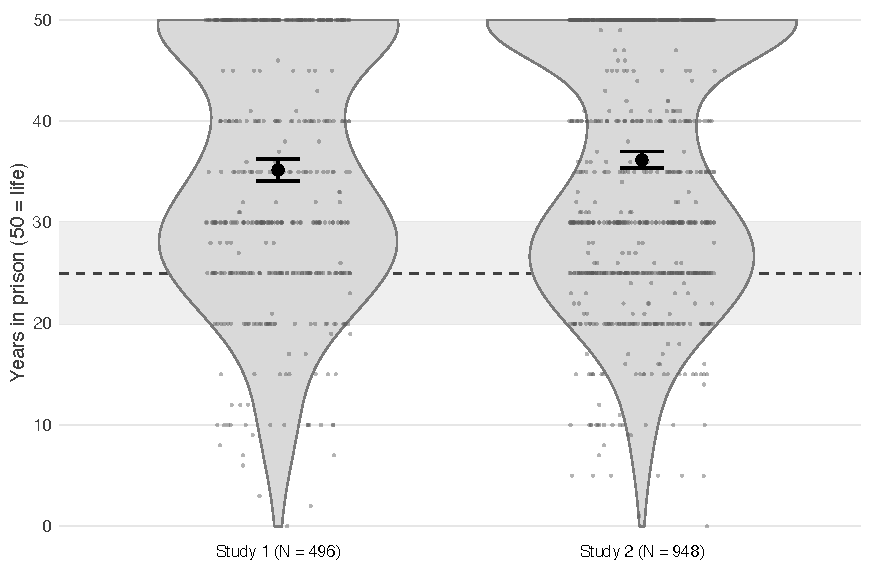
\includegraphics[width=\linewidth]{figures/fig5_sentences_both_studies.pdf}
\par\vspace{6pt}{\raggedright\figurenote{Violins show the distribution of sentences on the 0-to-50-year scale (50~= life). Small points are individual participants, jittered horizontally; large points are means with 95\% confidence intervals. The shaded band marks the 20-to-30-year range given in the instructions, and the dashed line marks its 25-year midpoint. The two distributions have much the same shape, with a concentration at the 50-year maximum, and in both studies more than half of participants chose a sentence above that range. Study 1 \emph{N}~=~496; Study 2 \emph{N}~=~948.}\par}
\end{figure}

% ---------------------------------------------------------------- Figure S2
\begin{figure}[!htbp]
\renewcommand{\thefigure}{S2}
\caption{Punitiveness and Its Correlates in Both Studies}
\label{fig:S2}
\centering
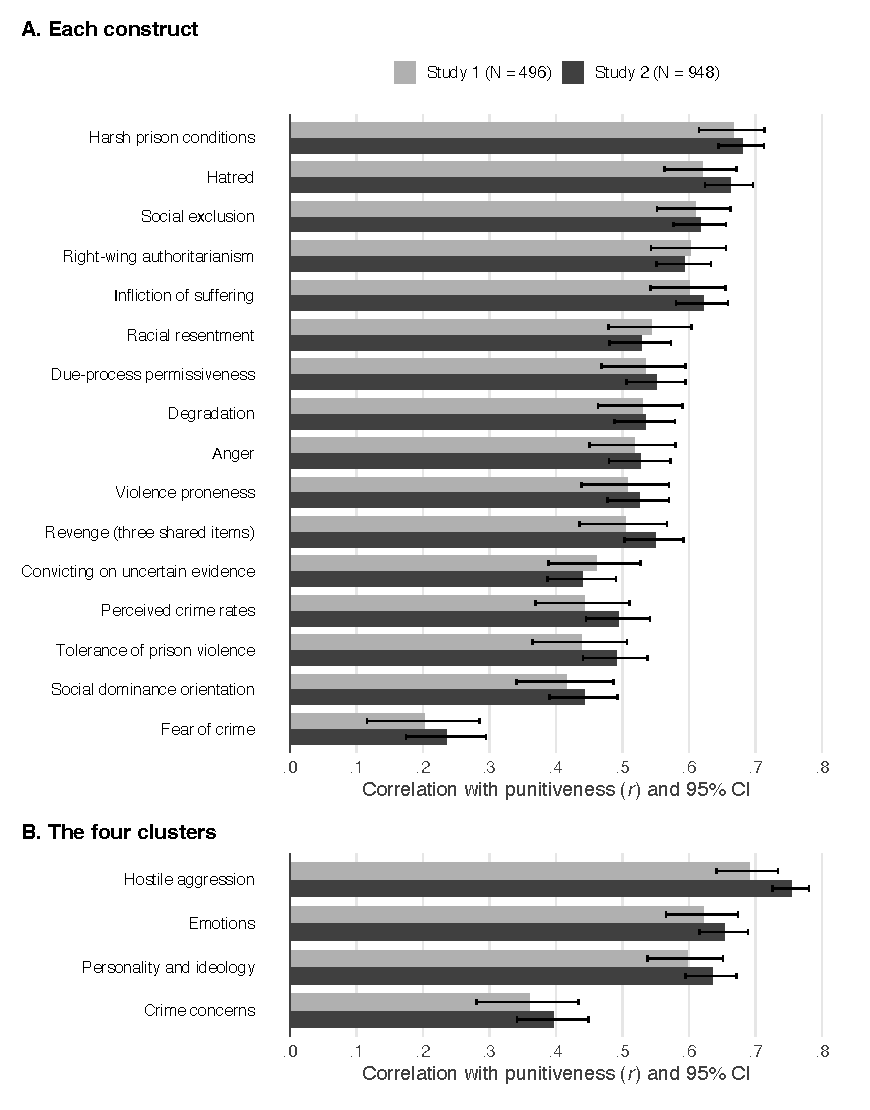
\includegraphics[width=\linewidth,height=0.72\textheight,keepaspectratio]{figures/fig6_correlates_both_studies.pdf}
\par\vspace{6pt}{\raggedright\figurenote{Bars show each correlate's correlation with punitiveness, with 95\% confidence intervals; light bars show Study 1 (\emph{N}~=~496) and dark bars Study 2 (\emph{N}~=~948). In both studies punitiveness is its six components (the five attitude components and the sentence), each standardized and weighted equally. Panel A shows the sixteen correlates both studies measured; Panel B shows the four clusters, each rebuilt in Study 2 from the individual items as Study 1 built it. Rows are ordered by the Study 1 correlation. Every correlate is positively related to punitiveness in both studies, and the sixteen correlations fall in closely matching order (Spearman ρ~=~.93). Revenge is scored with the three items both studies used. Study 1's personality and ideology cluster pools thirty items, including two measures Study 2 did not use; Study 2's cluster is built from the twenty-one items of the four measures the studies share. Built from those twenty-one items, Study 1's cluster correlates \emph{r}~=~.629 with punitiveness, just above emotions (.622).}\par}
\end{figure}

% ---------------------------------------------------------------- Figure S3
\begin{figure}[!htbp]
\renewcommand{\thefigure}{S3}
\caption{The Hostile Aggression Advantage in Both Studies}
\label{fig:S3}
\centering
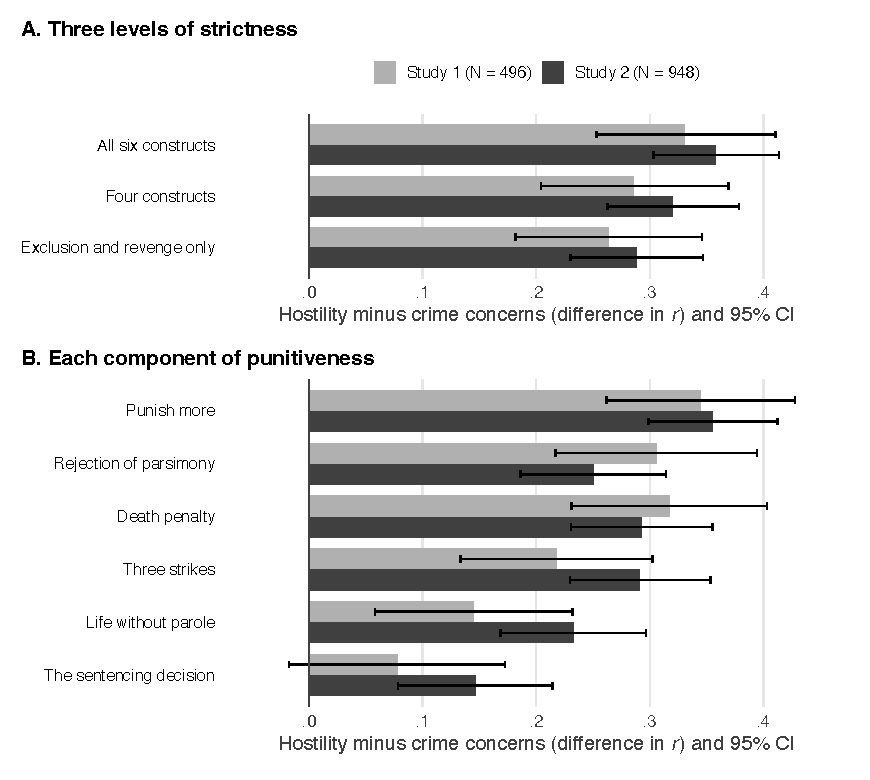
\includegraphics[width=\linewidth]{figures/fig7_hostility_advantage_both_studies.pdf}
\par\vspace{6pt}{\raggedright\figurenote{Bars show the difference between punitiveness's correlation with hostile aggression and its correlation with crime concerns, with 95\% confidence intervals; light bars show Study 1 (\emph{N}~=~496) and dark bars Study 2 (\emph{N}~=~948). Panel A shows the three levels of strictness of Table~S1: all six hostile aggression measures, four (infliction of suffering and harsh prison conditions dropped), and social exclusion and revenge only; in both studies punitiveness is its six components, each standardized and weighted equally. Panel B shows the comparison with all six hostile aggression measures on each of the six components of punitiveness separately. In both studies the clusters are built as Study 1 built them. The difference favors hostile aggression at every level and on every component; the one interval that includes zero is Study 1's for the sentencing decision. Intervals are Zou's (2007), computed the same way in both studies; for Study 1's three levels, Table~S1 and the Study 1 Results report bootstrap intervals instead, which differ slightly.}\par}
\end{figure}

% ---------------------------------------------------------------- Figure S4
\begin{figure}[!htbp]
\renewcommand{\thefigure}{S4}
\caption{Agreement With Proportionality and With Each Departure From It in Study 2 (H4 and H5)}
\label{fig:S4}
\centering
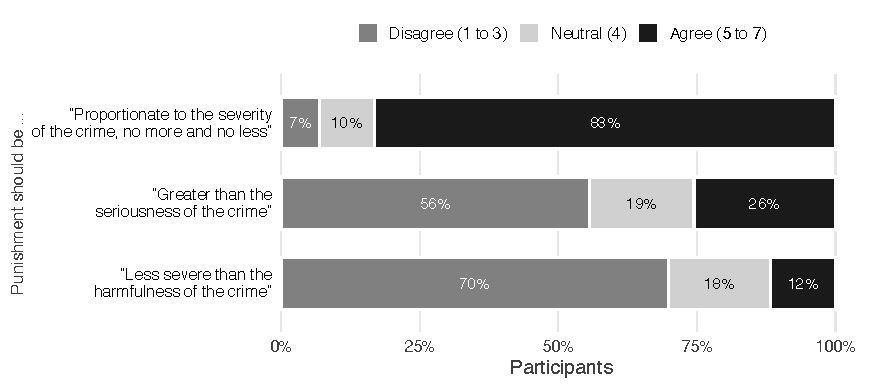
\includegraphics[width=\linewidth]{figures/fig9_study2_proportionality.pdf}
\par\vspace{6pt}{\raggedright\figurenote{For each of three statements about how severe punishment should be, bars show the share of participants who disagreed (1 to 3), were neutral (4), or agreed (5 to 7) on the scale from 1 (\emph{strongly disagree}) to 7 (\emph{strongly agree}). That punishment should be proportionate to the severity of the crime, no more and no less (the proportionality principle): 6.9\% disagreed, 10.0\% were neutral, and 83.1\% agreed. That it should be greater than the seriousness of the crime: 55.6\%, 18.9\%, and 25.5\%. That it should be less severe than the harmfulness of the crime: 69.8\%, 18.5\%, and 11.7\%. The two departure items are shown as answered, not reversed; the severity index averages the first of them with the second reversed. Segments are labeled with whole percentages, so a row's labels may not sum to 100. Table~S9 gives the H4 and H5 tests. \emph{N}~=~948.}\par}
\end{figure}

% ---------------------------------------------------------------- Figure S5
\begin{figure}[!htbp]
\renewcommand{\thefigure}{S5}
\caption{Endorsement of Desert Theory, Just Deserts, the Registered Just-Deserts Score, and Revenge, and Their Correlations With Punitiveness, in Study 2 (H9 and H10)}
\label{fig:S5}
\centering
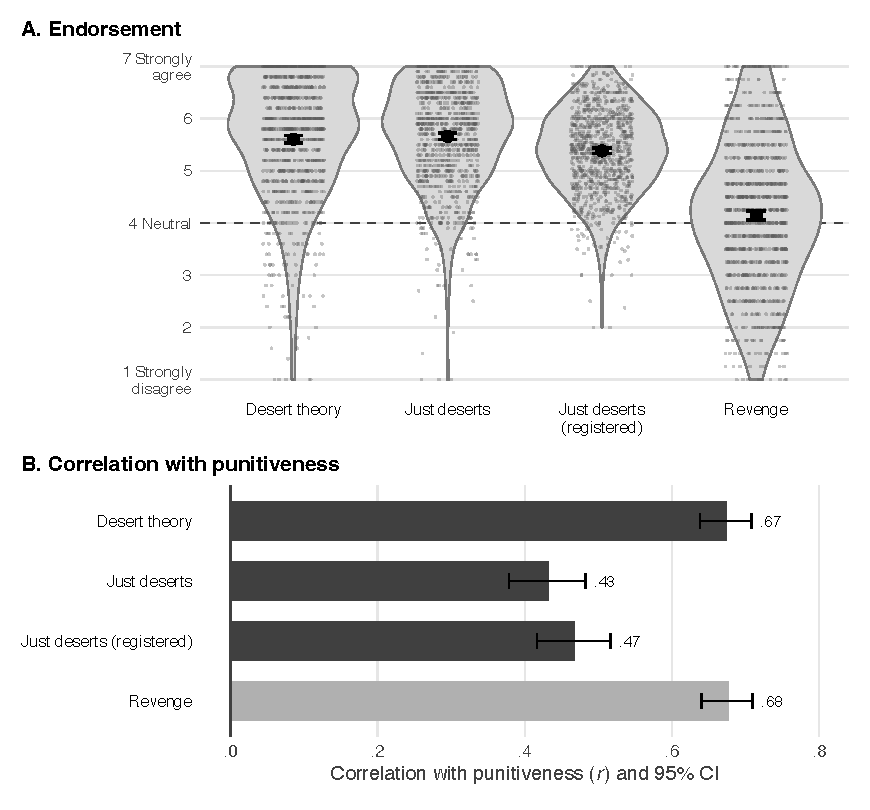
\includegraphics[width=\linewidth]{figures/fig12_study2_desert_revenge.pdf}
\par\vspace{6pt}{\raggedright\figurenote{Four scores are shown: desert theory, the mean of the five desert-theory items (\emph{M}~=~5.60); just deserts, the mean of desert theory and the proportionality principle (\emph{M}~=~5.66); the registered just-deserts score, which averages the registered desert score (items 1 to 4) with the three-item proportionality component (\emph{M}~=~5.38); and revenge, the mean of its four registered items (\emph{M}~=~4.14). Panel A shows each score on the 1-to-7 scale: violins show the distribution, small points are individual participants jittered horizontally, and large points are means with 95\% confidence intervals; the dashed line marks the neutral point. Panel B shows each score's correlation with punitiveness, the six-component score, with 95\% confidence intervals: .674 for desert theory, .432 for just deserts, .468 for the registered just-deserts score, and .676 for revenge. Dark bars are the three desert scores, and the light bar is revenge. The registered H9 and H10 tests used the registered just-deserts score, and H10 the eight-item scale (Table~S12). \emph{N}~=~948.}\par}
\end{figure}

% ---------------------------------------------------------------- Figure S6
\begin{figure}[!htbp]
\renewcommand{\thefigure}{S6}
\caption{How Far the Groupings of Retributivists Agree in Study 2}
\label{fig:S6}
\centering
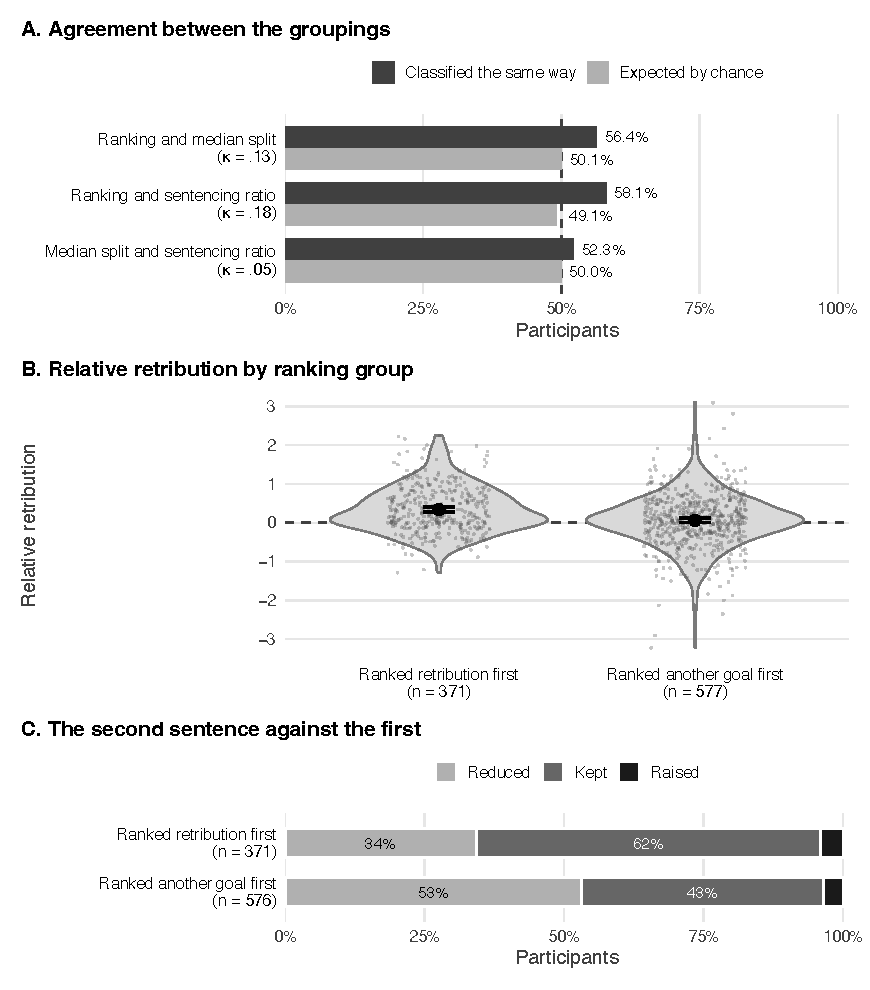
\includegraphics[width=\linewidth,height=0.72\textheight,keepaspectratio]{figures/fig14_study2_groupings.pdf}
\par\vspace{6pt}{\raggedright\figurenote{Panel A shows, for each pair of the three groupings that classify the whole sample (the sentencing-ratio split classifies all but one participant), the share of participants the two groupings place on the same side and the share expected by chance, with Cohen's κ; the dashed line marks 50\%. Panel B shows relative retribution, the mean of the seven-item retribution subscale minus the mean of the three other goals, for the participants who ranked retribution first and for everyone else: violins show the distribution, small points are individual participants jittered horizontally, and large points are means with 95\% confidence intervals; the dashed line marks retribution rated level with the other goals. Panel C shows the share of each ranking group that reduced, kept, or raised the sentence (\emph{n}~=~947); this grouping was not registered, and segments under 6\% are not labeled.}\par}
\end{figure}
